% Below is your UAH LaTeX template. This is the main file that compiles your document. You will need to fill out the appropriate sections below. 
\documentclass[oneside, 12pt]{book} % Document class


\usepackage[utf8]{inputenc} % Basic package for Latex
\usepackage{graphicx} % To help include figures
\usepackage{geometry} % To allow document margin changes
\usepackage{setspace} % To allow custom spacing 
\usepackage{indentfirst} % To allow indentations in the first paragraph.
\usepackage{amsmath,amssymb} % For formatting equations properly
\usepackage{natbib} % For formatting the bibliography
\usepackage{chngcntr} % To allow changing how figures, tables, and pages are counted.
\usepackage{appendix} % To help format the appendix
\usepackage[font=small,labelfont=bf]{caption} %This makes caption font small and makes the caption heading bold.
\usepackage{tabularx} %To allow formatting Tables.
\usepackage{array} %To allow creating arrays. 
\providecommand\phantomsection{} %This command allows you to make phantom sections that have no title but are still included in the Table of Contents such as the epigraph.
\usepackage[all]{nowidow} %This prevents widow/orphan lines
\usepackage{tikz}%This package helps to anchor the seal on the title page to the student name
\usetikzlibrary{tikzmark}%This is part of the tikz package
\usepackage{lscape,longtable}
\usepackage{multirow,multicol}

%Creating an Interlude Environment in order to NOT count or number a certain page such as the copyright page.
\newenvironment{interlude}{
  \clearpage
  \thispagestyle{empty}% we want this page to be empty (adjust to use a modified page style)
  \pagestyle{empty}% use the same style for subsequent pages in the unnumbered section
  }
  {\clearpage}

%The following package and lines can be used to format and create a list of symbols, equations, abbreviations, etc. The example actually used in this template is the \glossaries package, but you may also use this \nomencl package if desired.
\usepackage[intoc]{nomencl}
\makenomenclature
\renewcommand{\nomname}{List of Symbols}

% This is to ensure the page numbers are centered and at the bottom.
\usepackage{fancyhdr}
\pagestyle{fancy}
\fancyhf{}
\renewcommand{\headrulewidth}{0pt}
\cfoot{\thepage}

%This defines a new page style for just the title page.
\fancypagestyle{logopage}{\fancyhf{}\renewcommand{\headrulewidth}{0pt}\fancyfoot[C]{\includegraphics[scale=0.3]{Figures/Color Grad Banner.png}}}


\counterwithin{equation}{chapter} %this causes equations to be counted according to their chapter location
\counterwithin{figure}{chapter}




%This formats the table of contents the way Dr. Hakkila wants it
\usepackage[titles]{tocloft}


%Removes the Duplicate Chapter
\setcounter{secnumdepth}{4}% Show down to subsubsection

\setlength{\cftchapindent}{-20pt}% Just some value...

\usepackage{xpatch}

\makeatletter
\xpatchcmd{\@chapter}{\addcontentsline{toc}{chapter}{\protect\numberline{\thechapter}#1}}{%
                      \addcontentsline{toc}{chapter}{\protect\numberline{}#1}}{\typeout{Success}}{\typeout{Failed!}}
\makeatother



%This formats the Table of contents title
\renewcommand{\contentsname}{\hspace*{\fill}\bfseries\large Table of Contents\hspace*{\fill}}   


\renewcommand{\cftbeforetoctitleskip}{-0.25in}  

\renewcommand\cftchapdotsep{\cftdotsep}
\renewcommand\cftchapleader{\cftdotfill{\cftchapdotsep}}
%\renewcommand{\cftchappresnum}{CHAPTER } % put this before the number
%\addtolength{\cftchapnumwidth}{6em} % extra space for number and pre-name
%\renewcommand{\cftchapaftersnum}{. } % put period after chapter number and space


%This puts all the chapter headings into all-caps
%\renewcommand{\chaptername}{CHAPTER}

%Hopefully this reformats the List of Figures Title
\renewcommand{\listfigurename}{\hspace*{\fill}\bfseries\large List of Figures\hspace*{\fill}}  

%Reformat List of Tables, etc.
\renewcommand{\listtablename}{\hspace*{\fill}\bfseries\large List of Tables\hspace*{\fill}}  


%This creates a List of Equations.
\newcommand{\listequationsname}{List of Equations}
\newlistof{equations}{equ}{\listequationsname}

\newcommand{\eqdesc}[1]{%
  \csname phantomsection\endcsname % if hyperref is loaded
  \addcontentsline{equ}{equations}{\protect\numberline{\theequation}#1}%
}

\setlength{\parindent}{36pt}


%The following formats the chapter titles and sections appropriately
\usepackage{titlesec}



\titleformat
{\chapter}
[hang]
{\normalfont\large\bfseries\filcenter}
{} %Label. This is blank so that the entire chapter heading and title are properly centered. 
{0pt} %  Horizontal Space between label and title body.
{} %Before-Code 
{} 

\titleformat
{\section}
[hang]
{\normalfont\normalsize\bfseries}
{\thetitle} %Label. 
{.5em} %  Horizontal Space between label and title body.
{} %Before-Code 
{} 

\titleformat
{\subsection}
[hang]
{\normalfont\normalsize\bfseries}
{\thetitle} %Label. 
{.5em} %  Horizontal Space between label and title body.
{} %Before-Code 
{} 

\titlespacing{\subsection}{2em}{12pt}{12pt}

\titlespacing{\chapter}{0pt}{50pt}{12pt}

\titlespacing{\part}{0pt}{12pt}{12pt}


\titlespacing{name=\chapter, numberless}{0pt}{0pt}{12pt}


% I had used this code to combine the chapter heading and 
%\titleformat{\chapter}[hang] 
 % {\normalfont\large\bfseries\filcenter}{\chaptertitlename\ \thechapter:}{.3em}{} 


%This names the Bibliography/References whatever you want it to be.
\renewcommand{\bibname}{References}

%The below package creates the optional List of Symbols and formats it correction..
\usepackage[acronyms, automake, toc, nopostdot]{glossaries}
\usepackage{glossary-longbooktabs}
\newcolumntype{P}[1]{>{\centering\arraybackslash}p{#1}}
\renewcommand*{\entryname}{Symbol}
\newglossarystyle{mystyle}{% define custom glossaries style for Abbreviation page, read relative manual before change
\setglossarystyle{long-booktabs}%
\renewenvironment{theglossary}%
{\begin{longtable}{@{}P{3cm}@{}p{\dimexpr\linewidth-3cm}@{}}}%
{\end{longtable}}%

\renewcommand*{\glossaryheader}{%
 \bfseries\large Symbol & \centering\bfseries\large Description \tabularnewline\endhead \endfoot}%
}

\renewcommand{\glossarypreamble}{\normalsize}
\makeglossaries %To clean up this document, the preamble that includes the packages is located in the preamble.tex file found in the FrontMatter folder.




%********************************************
%********************************************
% THE SECTION BELOW MUST BE FILLED OUT 
%********************************************
%********************************************

%BASIC INFORMATION
\newcommand{\thesistitle}{TITLE}
\newcommand{\studentname}{Rebecca Harvey}
\newcommand{\degree}{Doctor of Philosophy}%e.g., Master of Science in Engineering, Doctor of Philosophy, etc.
\newcommand{\department}{Space Science}% Do not include the words "The department of." Just write the name of your department.
\newcommand{\gradyear}{2025}% complete 4 digit year, e.g., 2022
\newcommand{\gradmonth}{June}% Spell out the month completely, e.g., December
%\newcommand{\jointuni}{Auburn University} %If this is a joint degree, remove the % sign at the beginning of this line and enter the entire name of the additional universities.

%***********************
%SPECIFY THESIS OR DISSERTATION
% Below, if you are earning a master's degree, remove the "%" on the line below that says \newcommand{thesis}. If you are earning a PhD or other doctorate degree, remove the "%" on the line below that says \newcommand{dissertation}.

%\newcommand{\thesis}{FOR MASTER'S STUDENTS ONLY}
\newcommand{\dissertation}{FOR DOCTORATE DEGREE STUDENTS ONLY}

%*******************************
%SPECIFY THE PROFESSORS WHO WILL APPROVE YOUR THESIS/DISSERTATION
%Professor information: Fill out only their first and last name WITH NO PREFIXES OR SUFFIXES. If a line is not applicable, simply add a % sign at the beginning of that line. If there is an applicable line that has a % sign at the beginning, remove this sign and fill in as needed.
%\newcommand{\resadv}{[Research Advisor Name]}
%\newcommand{\comchair}{[Committee Chair Name]}
\newcommand{\reschair}{Qiang Hu} %If your research advisor and committee chair are the same person, enter his/her name on this line.
\newcommand{\commema}{[Gary Zank]}
\newcommand{\commemb}{[Linling Zhao]}
\newcommand{\commemc}{[Jakobus le Roux]}
\newcommand{\commemd}{[Laxman Adhikari]}
%\newcommand{\commeme}{[5th Committee Member Name]}
%\newcommand{\commemf}{[6th Committee Member Name]}
%\newcommand{\commemg}{[7th Committee Member Name]}
%\newcommand{\commemh}{[8th Committee Member Name]}
%\newcommand{\commemi}{[9th Committee Member Name]}
\newcommand{\depchair}{[Vladimir Florinksi]}
\newcommand{\colldean}{[Rainer Steinwandt]}
\newcommand{\graddean}{Jon Hakkila}



%**************
%INDICATE IF YOU HAVE REGISTERED FOR A COPYRIGHT.
%**************
%\newcommand{\copyrightreg}{Yes} %If you registered for a copyright through Proquest, please remove the % sign from the beginning of this line starting with \newcommand{\copyrightreg}{Yes}. If you did not register for a copyright, no action is needed.  

%********************************************
%********************************************
% End of Section to Fill Out. 
%********************************************
%********************************************

\usepackage[colorlinks=true,linkcolor=black,anchorcolor=black,citecolor=black,filecolor=black,menucolor=black,runcolor=black,urlcolor=black]{hyperref} %This creates hyperlinks for chapter, figure, and table titles in your pdf. It should be the last package before the document begins.
\usepackage[toc,page]{appendix}
%*********************************************
%*********************************************
%Optional List of Symbols/Abbreviations
%*********************************************
%*********************************************

%A list of symbols/abbreviations is optional. If you do not want to include one, simply delete this section from your document. You may also delete this section and use a different package as there are multiple packages that can be used to make a List of Symbols, Abbreviations, Nomenclature, Etc. Below uses the \glossaries-extra package. This package is nice if you want to include multiple lists or sections. The following links provide useful information on how to use this package.
% https://mirrors.mit.edu/CTAN/macros/latex/contrib/glossaries/glossariesbegin.pdf
% https://mirrors.rit.edu/CTAN/macros/latex/contrib/glossaries/glossaries-user.pdf
% https://www.overleaf.com/learn/latex/Glossaries


% This uses the glossaries package. With this package, you can include multiple types of lists, track page numbers if desired, and define new lists. More information can be found at the following sites: https://mirrors.mit.edu/CTAN/macros/latex/contrib/glossaries/glossariesbegin.pdf and https://mirrors.rit.edu/CTAN/macros/latex/contrib/glossaries/glossaries-user.pdf https://www.overleaf.com/learn/latex/Glossaries


%*****************************************
%Define your list of glossary items below. Remember that the entries that you enter in this file will not automatically appear in the List of Symbols. You also have to reference the symbol in the body of your thesis by using the \gls command. 

%symbols
% \newglossaryentry{deg}{name=$^\circ$, description={Degree}}
% \newglossaryentry{grav}{name={1D}, description={Normal gravity environment}}
% \newglossaryentry{wf}{name={\textit{f}}, description={Wear factor}}
% \newglossaryentry{alp}{name={$\alpha$},description={Alpha}}
% \newglossaryentry{theta}{name={$r_O$}, description={ecosystem respiration at reference temperature $T_a=0{^\circ}$C}}
% \newglossaryentry{te}{name={$\tau_e$}, description={precision of the normal distribution of the likelihood}}
% \newglossaryentry{q10}{name={$Q_{10}$}, description={multiplication factor to respiration with 10$^\circ$C increases in $T_a$}}
% \newglossaryentry{phi}{name={$\phi$}, description={vapour pressure deficit response function}}
% \newglossaryentry{del}{name=$\delta$, description={Transition coefficient constant for the design of linear-phase FIR filters which are used to take up space when testing the list of symbols}}

\newglossaryentry{MMS}{name=MMS, description={Magnetospheric Multiscale mission}}
\newglossaryentry{THEMIS}{name=THEMIS, description={Time History of Events and Macroscale Interactions during Substorms mission}}

\newglossaryentry{RE}{name=$R_E$, description={Radius of the Earth, 6372 km}}
\newglossaryentry{AU}{name=AU, description={Astronomical unit: distance between the Earth and the sun, 1.4959$\times 10^8$ km}}
\newglossaryentry{GSE}{name=GSE, description={Geocentric Solar Ecliptic coordinate system}}

\newglossaryentry{IMF}{name=IMF, description={Interplanetary magnetic field}}
\newglossaryentry{SFR}{name=SFR, description={small-scale flux rope}}

\newglossaryentry{GS}{name=GS, description={Grad-Shafranov}}
\newglossaryentry{magnetic flux function}{name=$A$, description={magnetic flux function}}
\newglossaryentry{transformed magnetic flux function}{name=$A'$, description={modified magnetic flux function}}
\newglossaryentry{transverse pressure}{name=$P_t'(A')$, description={transverse pressure as a function of the modified magnetic flux function}}
\newglossaryentry{Rdiff}{name=$R_{diff}$, description={point-wise difference residue between the two parts}}
\newglossaryentry{Rfit}{name=$R_{fit}$, description={residue of the fitting function $P_t'(A')$}}
\newglossaryentry{walen}{name=$w$, description={Wal\'en test slope}}

\newglossaryentry{axial flux}{name=$\Phi_z$, description={approximate axial magnetic flux}}
\newglossaryentry{poloidal flux}{name=$|A_m|$, description={poloidal magnetic flux per meter}}

\newglossaryentry{sigma_c}{name=$\sigma_c$, description={normalized cross helicity}}
\newglossaryentry{sigma_m}{name=$\sigma_m$, description={normalized magnetic helicity}}
\newglossaryentry{sigma_r}{name=$\sigma_r$, description={normalized residual energy}}
\newglossaryentry{phi}{name={$\phi$}, description={azimuthal angle between the GSE $X$-direction and the projection of the $z$-axis onto the $XY$-plane}}
\newglossaryentry{theta}{name={$\theta$}, description={polar angle between the SFR $z$-axis and the GSE $Z$-direction}}
\newglossaryentry{alpha}{name={$\alpha$},description={ average Alfv\'en Mach number squared}} %Go to this page to enter all the symbols you plan to use in the document.

% Scroll down in this file to after the List of Tables section in order to actually add your Lists to your document,.

%**********************************************
%**********************************************
% End of Optional List of Symbols/Abbreviations
%**********************************************
%**********************************************

% math and equations commands
\newcommand{\del}{\nabla}
\newcommand{\cross}{\times}
\newcommand{\p}[1]{\left( #1 \right)}
\newcommand{\pp}[1]{\left[ #1 \right]}
\newcommand{\psq}[1]{\left \{ #1 \right \} }
\newcommand{\pang}[1]{\left \langle #1 \right\rangle }
\def\cross{\times}
\def\grad{\nabla}
\def\delcross{\nabla \times}
\def\deldot{\nabla \cdot}
\def\delsq{\nabla^2}
\newcommand{\dv}[2]{\frac{d #1}{d #2}}
\newcommand{\pdv}[2]{\frac{\partial #1}{\partial #2}}
\newcommand{\npdv}[3]{\frac{\partial^{#1} #2}{\partial #3^{#1}}}
\newcommand{\eq}[1]{\begin{equation*} #1 \end{equation*}}
\newcommand{\eql}[2]{\begin{equation} \label{#1} #2 \end{equation}}

\def\Avec{\mathbf{A}}
\def\Bvec{\mathbf{B}}
\def\bvec{\mathbf{b}}
\def\jvec{\mathbf{j}}
\def\xhat{\hat{x}}
\def\zhat{\hat{z}}
\def\psihat{\hat{\psi}}


%******************************************
%******************************************
% Document Begins Here
%******************************************
%******************************************

\begin{document}

\frontmatter % This command creates the front matter environment.

%**********************************
%**********************************
%Title Page
%**********************************
%**********************************
% Do not directly edit this page. Everything on the Title Page should auto-fill if you correctly filled out the information on the main.tex file.

\begin{titlepage}
\newgeometry{left=1.5in,bottom=.5in}
    \begin{center}
        \Large
        \singlespacing
        \textbf{\thesistitle}
        

\vspace{2cm}

        \large
        \textbf{\studentname}\\
        \vspace{1.5cm}
        \normalsize
        \ifdefined\thesis
        \textbf{A THESIS}
        \vspace{1.5cm}
        \else
        \ifdefined\dissertation
        \textbf{A DISSERTATION}
        \vspace{1.5cm}
        \else
        Please identify this document as either a thesis or dissertation on the main.tex file in the section at the top that must be filled out.
        \vspace{1.5cm}
        \fi
        \fi

        \textbf{Submitted in partial fulfillment of the requirements \\for the degree of \degree}\\  
        
\vspace{0.1cm}
  \textbf{in}\\
      \vspace{0.1cm}
        \textbf{The Department of \department}\\
        \vspace{0.1cm}
  \textbf{to}\\
\vspace{0.1cm}
\textbf{The Graduate School}\\
\vspace{0.1cm}
\textbf{of}\\
\vspace{0.1cm}
        \ifdefined\jointuni
        \textbf{The University of Alabama in Huntsville\\ and\\  \jointuni}
        \else
        \textbf{The University of Alabama in Huntsville}
    \fi

        
        \vspace{0.4cm}
        \textbf{\gradmonth\ \gradyear}
        


    \end{center}
    

\vfill

\textbf{Approved by:}


\vspace{.1cm}
\setstretch{1.25}

\ifdefined\reschair
\noindent
Dr. Qiang Hu, Research Advisor/Committee Chair\\
\else
\noindent
Dr. \resadv, Research Advisor \\
Dr. \comchair, Committee Chair\\
\fi
\ifdefined\commemi
\noindent
Dr. \commema, Committee Member\\
Dr. \commemb, Committee Member\\
Dr. \commemc, Committee Member\\
Dr. \commemd, Committee Member\\
Dr. \commeme, Committee Member\\
Dr. \commemf, Committee Member\\
Dr. \commemg, Committee Member\\
Dr. \commemh, Committee Member\\
Dr. \commemi, Committee Member\\
Dr. \depchair Florinski, Department Chair\\
Dr. \colldean, College Dean\\
Dr. \graddean, Graduate Dean\\
\else
\ifdefined\commemh
\noindent
Dr. \commema, Committee Member\\
Dr. \commemb, Committee Member\\
Dr. \commemc, Committee Member\\
Dr. \commemd, Committee Member\\
Dr. \commeme, Committee Member\\
Dr. \commemf, Committee Member\\
Dr. \commemg, Committee Member\\
Dr. \commemh, Committee Member\\
Dr. \depchair, Department Chair\\
Dr. \colldean, College Dean\\
Dr. \graddean, Graduate Dean\\
\else
\ifdefined\commemg
\noindent
Dr. \commema, Committee Member\\
Dr. \commemb, Committee Member\\
Dr. \commemc, Committee Member\\
Dr. \commemd, Committee Member\\
Dr. \commeme, Committee Member\\
Dr. \commemf, Committee Member\\
Dr. \commemg, Committee Member\\
Dr. \depchair, Department Chair\\
Dr. \colldean, College Dean\\
Dr. \graddean, Graduate Dean\\
\else
\ifdefined\commemf
\noindent
Dr. \commema, Committee Member\\
Dr. \commemb, Committee Member\\
Dr. \commemc, Committee Member\\
Dr. \commemd, Committee Member\\
Dr. \commeme, Committee Member\\
Dr. \commemf, Committee Member\\
Dr. \depchair, Department Chair\\
Dr. \colldean, College Dean\\
Dr. \graddean, Graduate Dean\\
\else
\ifdefined\commeme
Dr. \commema, Committee Member\\
Dr. \commemb, Committee Member\\
Dr. \commemc, Committee Member\\
Dr. \commemd, Committee Member\\
Dr. \commeme, Committee Member\\
Dr. \depchair, Department Chair\\
Dr. \colldean, College Dean\\
Dr. \graddean, Graduate Dean\\
\else
\ifdefined\commemd
Dr. \commema, Committee Member\\
Dr. \commemb, Committee Member\\
Dr. \commemc, Committee Member\\
Dr. \commemd, Committee Member\\
Dr. \depchair, Department Chair\\
Dr. \colldean, College Dean\\
Dr. \graddean, Graduate Dean\\
\else
\ifdefined\commemc
Dr. \commema, Committee Member\\
Dr. \commemb, Committee Member\\
Dr. \commemc, Committee Member\\
Dr. \depchair, Department Chair\\
Dr. \colldean, College Dean\\
Dr. \graddean, Graduate Dean\\
\else
\ifdefined\commemb
Dr. \commema, Committee Member\\
Dr. \commemb, Committee Member\\
Dr. \depchair, Department Chair\\
Dr. \colldean, College Dean\\
Dr. \graddean, Graduate Dean\\
\else
\ifdefined\commema
Dr. \commema, Committee Member\\
Dr. \depchair, Department Chair\\
Dr. \colldean, College Dean\\
Dr. \graddean, Graduate Dean\\
\else
Dr. \depchair, Department Chair\\
Dr. \colldean, College Dean\\
Dr. \graddean, Graduate Dean\\
\fi
\fi
\fi
\fi
\fi
\fi
\fi
\fi
\fi
\end{titlepage}


\restoregeometry%Your title page should self-generate after filling in the required information above.
\newpage

%This sets the page margins. If you plan to bind and print your thesis, change the left boarder to 1.5 in.
\newgeometry{left=1.5in, right=1in, bottom=1in, top=1in}
\setcounter{page}{2} 
%**********************************
%**********************************
%Abstract Page
%**********************************
%**********************************

%The below code inserts your Abstract Page. While much of this page fills in automatically, you must go to the AbstractPage.tex file located in the FrontMatter folder and insert the actual text of your abstract. 

% The top of your abstract will fill out automatically once you fill in the required fields on the main.tex file. In this file, you will provide your abstract body. Type your abstract body at the bottom of this page directly below the \doublespacing command.

\chapter{Abstract}
     \begin{center}
        \large
        \singlespacing
        \textbf{\thesistitle}\\
        \vspace{0.5cm}
        \large
        \textbf{\studentname}\\
        \vspace{0.5cm}
        \normalsize
        \ifdefined\thesis
        \textbf{A thesis submitted in partial fulfillment of the requirements \\for the degree of \degree}\\  
        \else
        \ifdefined\dissertation
        \textbf{A dissertation submitted in partial fulfillment of the requirements \\for the degree of \degree}\\
        \else
        \textbf{Please identify this document as either a thesis or dissertation on the main.tex in the section at the top that must be filled out.}\\
    \fi
    \fi
        \vspace{1cm}
        \textbf{\department}
        
        \vspace{0.25cm}

        \ifdefined\jointuni
        \textbf{The University of Alabama in Huntsville and  \jointuni}
        \else
        \textbf{The University of Alabama in Huntsville}
    \fi

        
        \vspace{0.1cm}
        \textbf{\gradmonth\ \gradyear}
        


    \end{center}
\vspace{0.1cm}

%****************************************************
%Enter the body of your abstract below. Remember there is a 150 word limit!
%****************************************************
\doublespacing
This dissertation work identifies and characterizes magnetic structures in the solar wind and magnetosheath across the Earth's bow shock. I investigate the differences between the properties of small-scale flux rope (SFR) structures immediately upstream and downstream of the bow shock by employing two data analysis methods: one based on wavelet transforms and the other based on the Grad-Shafranov (GS) detection and reconstruction techniques. In situ magnetic field and plasma data from the Magnetospheric Multiscale (MMS) and Time History of Events and Macroscale Interactions during Substorms (THEMIS) missions are used to identify these coherent structures. 

Previous studies of SFRs have used the extended Grad-Shafranov GS based techniques for the solar wind plasma; however, this algorithm was not used in other regions of near-Earth space such as the magnetosheath. Furthermore, many studies regarding flux ropes and other magnetic structures focus on events identified during specific periods of time, instead of seeking to use multiple spacecraft for a study coordinated in the immediate regions across the bow shock. I characterize magnetic structures with varying degrees of Alfv\'enicity as they move across boundaries in near-Earth space. As I investigate the difference between the properties of the magnetic structures in different near-Earth regions, our aim is to characterize the types of magnetic structures that are identified in the magnetosheath and solar wind in a systematic manner. I identify thousands of SFR event intervals over a total time period of $\sim$1000 hours in each region, and an inventory of events with high magnetic helicity is provided. I report the parameters associated with the SFRs such as scale size, duration, magnetic flux content, and magnetic helicity density, and a direct comparison of the statistical properties of the structures from these two regions is performed.

\clearpage



%**********************************
%**********************************
%Copyright Page
%**********************************
%**********************************

% The following code inserts your COPYRIGHT page. If you have registered for a copyright through Proquest, you should have removed the % sign from the \newcommand{copyrightreg} at the end of the section to Fill Out. If you have not registered for a copyright, no action is needed.
\ifdefined\copyrightreg
\doublespacing
\begin{center}

    \vspace*{\fill}

\copyright \\
\studentname \\
All Rights Reserved
\end{center}
\else
\newpage
\
\newpage
\fi



%**********************************
%**********************************
%Acknowledgements
%**********************************
%**********************************

% Your acknowledgements are included here. Similar to the abstract, you must open the Acknowledgements.tex file located in the FrontMatter folder to type your acknowledgements.
% Type your Acknowledgements below. Delete all the text after the double-spacing command.
\chapter{Acknowledgements}
\doublespacing

% If you wish, you may also thank family or friends. You may conclude your acknowledgments with a dedication rather than using a separate dedication page. Your acknowledgments should be brief and consistent in tone with a formal publication.

% \begin{itemize}
%     \item Clayton
%     \item Dorrine
%     \item Sarah, Kat, Juan, Michael, Keyvan, Keaton, Sydney
%     \item Cori
%     \item Family
% \end{itemize}

% To my partner Clayton: Words can't even describe how grateful I am for the support that you've given me.

% To my best work-from-home buddy Dorrine: You were supposed to be here to see it all through, but life had other plans. Thank you for your many, loud suggestions and moral support snuggles. After all, you did try to type some of this document yourself.

% To my friends and co-workers Sarah, Kat, Juan, Michael, Keyvan, Keaton, and Sydney: 

% You must pay your scholarly debts by thanking those who have provided intellectual guidance, facilities, or financial support for your project; thus, you thank those who have been significantly involved in your work. You must acknowledge any agency providing funding or other resources, and any individual or institution who has granted you permission to reprint material.

% \begin{itemize}
%     \item Advisor
%     \item Committee
%     \item Yu Chen
% \end{itemize}

Personal acknowledgements \\

This work is funded by NASA Grants 80NSSC21K0003, 80NSSC21K1763, 80NSSC21K1319, and NSF Grant AGS‐2229065. I acknowledge NASA contract NAS5-02099 and V. Angelopoulos for use of data from the THEMIS Mission. Specifically: K. H. Glassmeier, U. Auster and W. Baumjohann for the use of FGM data \citep{Auster:2008} provided under the lead of the Technical University of Braunschweig and with financial support through the German Ministry for Economy and Technology and the German Center for Aviation and Space (DLR) under contract 50 OC 0302, and C. W. Carlson and J. P. McFadden for use of ESA \citep{McFadden:2008} data. I thank the individuals who support the MMS mission, specifically that of the FIELDS team \citep{Torbert:2016} and the FPI team \citep{Pollock:2016}, as well as those who make the data readily available. I would like to gratefully acknowledge Wenli Mo and Savvas Raptis for their correspondence providing the MMS data set classified in different magnetospheric regions. 





%The code below formats your table of contents, list of figures, list of tables, and list of symbols. If your document does not contain any figures and/or tables, simply delete that section. The list of symbols is optional. Again, delete that section if you do not want to include it in your document.

%*************************
%Table of Contents Section
%*************************
\newgeometry{left=1.75in}%For some reason, I have to set only the Table of Contents to a left margin of 1.75 so that everything lines up correctly.
{\renewcommand\uppercase[1]{#1} % This creates an environment to NOT put titles in all-caps
\singlespacing
\setlength{\cftparskip}{1\baselineskip}% This single-spaces within entries and double-spaces between them.
\tableofcontents %Command to create the table of contents
\addcontentsline{toc}{chapter}{Table of Contents} %Changes the name from Contents to Table of Contents
\newpage %Creates a page break before the next section.

%*************************
%List of Figures Section
%*************************
\newgeometry{left=1.5in}
\cleardoublepage\phantomsection\addcontentsline{toc}{chapter}{List of Figures} %Adds the List of figures to the Table of contents.
\singlespacing
\setlength{\cftparskip}{.5\baselineskip} %This allows single space within entries and double space between them.
\listoffigures %This command creates the list of figures.
\newpage %Creates a page break before the next section.

%*************************
%List of Tables Section
%*************************
\newgeometry{left=1.5in}
\cleardoublepage\phantomsection\addcontentsline{toc}{chapter}{List of Tables} %Adds the List of figures to the Table of contents. The \clear doublepage and \phantomsection make the links work properly.
\singlespacing
\setlength{\cftparskip}{.5\baselineskip} %This allows single space within entries and double space between them.
\listoftables %This command creates the list of tables.
\newpage
}


%**************************
%List of Symbols Section
%**************************
\singlespacing
\renewcommand*{\arraystretch}{2}
\printglossary[title=\centering List of Symbols, toctitle=List of Symbols,style=mystyle,nonumberlist]



%Include your epigraph here if you have one by removing the % sign on the lines of code below and then typing in the required information on the epigraph page. Go to the epigraphOptional.tex file found in the FrontMatter folder. 

\clearpage \phantomsection \addcontentsline{toc}{chapter}{Epigraph} % This page is optional. If you plan to include it, simply insert your quote and the author in the appropriate locations below. 
\newgeometry{top=2in}
\begin{center}
    \textit{Ask me what I learned from all those years, \\ Ask me what I earned from all those tears, \\ Ask me why so many fade, but I'm still here}
\end{center}
\begin{flushright}
- ``Karma" by Taylor Swift (Midnights)
\end{flushright}
\restoregeometry

%************************
%Body of your Thesis Begins
%************************
\mainmatter

\newgeometry{left=1.5in}
\doublespacing
%The contents of your chapters are located in separate chapter.tex files. This template only contains 3 chapter files (ch1, ch2, and chLast). To edit these files, open the corresponding chapter.tex files. To create new chapters, make a new .tex file for each chapter and then insert them into your document below with the \include{name of your chapter .tex file} command.

\chapter{Chapter 1. Introduction}

\section{Space Environment}

\subsection{Interplanetary magnetic field and near-Earth solar wind}
It was proposed by \cite{Parker:1958} that there was gas pushed radially outward from the sun, called solar wind, reaching typical speeds of 400-800 km/s. As a spacecraft traverses near-Earth space, it moves from the solar wind through the different regimes of the terrestrial magnetosphere, which is the spatial domain of the magnetic-field lines that connect to the Earth \citep{Borovsky:2018}. Before experiencing the near-Earth regime, the particles emitted from the sun move through the interplanetary medium, and are subject to the magnetic field of the sun. The interplanetary magnetic field (\gls{IMF}) is the magnetic field of the sun that is carried out in the solar system by the solar wind. The IMF takes the shape of an Archimedean spiral due to the rotation of the sun, as seen in Figure \ref{fig:IMF-spiral}.

\begin{figure}
    \centering
    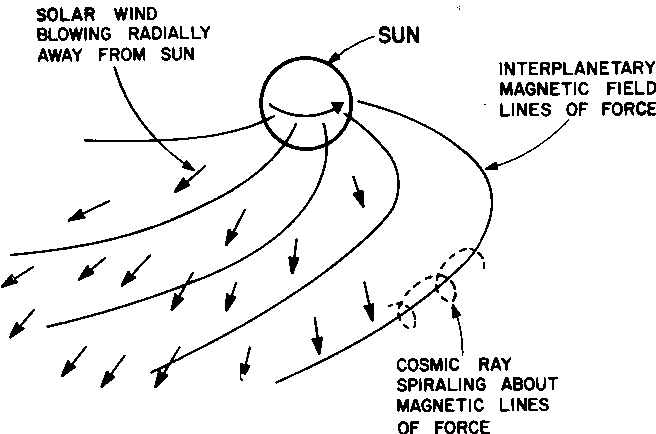
\includegraphics[width=\linewidth]{Figures/IMF.png}
    \caption[Diagram of the interplanetary magnetic field]{The IMF is carried away from the sun by the solar wind in an Archimedean spiral \citep{Mccracken:1967}.}
    \label{fig:IMF-spiral}
\end{figure}

\noindent The charged particles in the solar wind, primarily electrons and protons (ionized hydrogen), stream outward from the sun with the spiral field lines of the IMF. When the IMF meets the Earth's magnetic field, these particles can enter the magnetosphere and cause phenomena such as auroras and geomagnetic storms. 

In general, solar wind streams can be divided into the fast and slow solar wind. Fast solar wind originates from coronal holes, while slow solar wind originates near the solar equator from coronal streamers. Other variations in solar wind properties can be caused by solar wind transients, such as coronal mass ejections. Coronal mass ejections release energetic plasma from the sun into interplanetary space, and this release can perturb the solar wind. In near-Earth space ($\sim$1 \gls{AU}), the solar wind velocity is observed to be approximately 200-800 km/s. As the solar wind encounters the magnetic field of Earth, it is mostly deflected around the Earth's magnetosphere. The solar wind that enters the magnetosphere sees a significant drop in velocity, but an increase in density.

\subsection{Bow shock}
The magnetosphere presents an obstacle to the flow of the solar wind, and as the solar wind rapidly decelerates from supersonic flow into a subsonic flow, a standing fast shock is formed upstream of Earth \citep{Dimmock:2013}. The plasma is deflected around the magnetosphere as it reaches the bow shock. The bow shock is a collisionless shock that forms from the interaction of the solar wind with Earth's magnetic field. It forms a parabolic boundary around the Earth, with the nose being approximately 15 \gls{RE} in distance in the sunward direction. However, this boundary is constantly moving due to changing solar wind properties. Many studies have used statistics \citep{Kruparova:2019}, machine learning techniques \citep{Lalti:2022}, or empirical models \citep{chapman_three-dimensional_2003} to identify and locate bow shock crossings of different spacecraft. The interaction of the solar wind with the bow shock can generate magnetic islands and other structures \citep{Karimabadi:2014} in the downstream magnetosheath, and interactions within the magnetosheath lead to wave generation and dissipation, magnetic reconnection, and turbulence \citep{Shaikh:2022}. %As structures and 

\subsection{Magnetosheath}
The magnetosheath is a region of shocked, turbulent, highly magnetized plasma that forms directly downstream of the bow shock. The flow of the solar wind is impeded by the Earth's magnetic field; therefore, the compressed, heated, and turbulent solar wind gets wrapped around Earth's magnetic field. This interface between Earth's terrestrial magnetosphere and the solar wind plays a significant role in the flow of particles across these boundaries. Plasma in the magnetosheath experiences large fluctuations, and \cite{Hadid:2018} estimates that the average energy cascade rate within the magnetosheath is approximately two orders of magnitude larger than the solar wind. The geometry of the bow shock and the interplanetary magnetic field determines the plasma dynamics of the magnetosheath \citep{Yordanova:2020}. Under a quasi-perpendicular angle of the shock normal ($>45^\circ$), the plasma experiences a sharp decrease in the velocity and sharp increase in the magnitude of the magnetic field. The temperature anisotropy is typically larger in the quasi-perpendicular region, and the quasi-perpendicular region has lower energy flux than the quasi-parallel region \citep{Gurchumelia:2022}. This turbulent layer of plasma is bounded by the magnetopause, which is the outer boundary that separates the solar wind from the magnetosphere. 
%Under a quasi-parallel angle of the shock normal ($<45^\circ$), the IMF is connected to the Earth's magnetic field, allowing particles to more easily enter the Earth's terrestrial magnetosphere. One such region which is under a quasi-parallel shock normal is the foreshock region, which is the region in between the last interplanetary field line that connects to the bow shock and the bow shock itself \citep{Karlsson:2021}. In the foreshock region, many solar wind particles are reflected by the bow shock, causing instabilities and other upstream phenomena, which in turn creates intense wave activity \citep{turc_transmission_2023}, such as fast magnetosonic waves \citep{Anderson:1994}.

\subsection{Magnetopause}
The magnetopause is the boundary at which the solar wind dynamic pressure is approximately equal to the pressure of Earth's magnetic field \citep{Shue:1997}. Because the pressure is not static, the magnetopause boundary moves in relation to the solar wind properties. The standoff distance of the magnetopause nose can be estimated by taking the solar wind ram pressure and setting it equal to the magnetic pressure of Earth's magnetic field. This distance is typically 6-15 $R_E$, based on solar wind conditions \citep{Collado-Vega:2023}. Figure \ref{fig:magnetopause} shows an overview of the bow shock and magnetopause boundaries, as well as a representation of the flow of plasma (black arrows). 

\begin{figure}
    \centering
    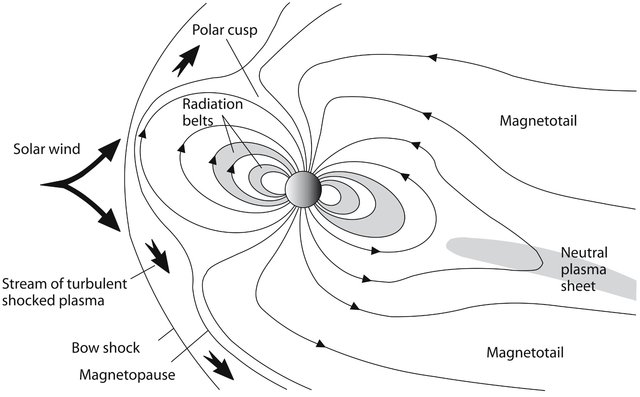
\includegraphics[width=\linewidth]{Figures/The-magnetosphere-is-the-region-where-Earths-magnetic-field-predominates-The_W640.jpg}
    \caption[Diagram of the Earth's magnetopause and magnetic field lines.]{Diagram of the magnetopause and Earth's magnetic field lines \citep{Anderson:2018}. The thick arrows show the direction of the flow of plasma as it enters the magnetosheath and is wrapped around the magnetosphere. The non-uniform shape of the magnetopause can be seen.}
    \label{fig:magnetopause}
\end{figure}

The magnetopause acts as a sieve, allowing charged particles to enter the magnetosphere. Energetic particles entering the terrestrial magnetosphere leads to geomagnetic activity and has implications for space weather. Positive (negative) ions (electrons) that drift westward (eastward) contribute to the ring current, which affects the strength of a geomagnetic storm \citep{Williams:1981}. Magnetic reconnection at the magnetopause injects magnetic flux into the tail region of the magnetosphere \citep{Tsurutani:1990}. Vortices at the edges of the magnetopause, e.g. Kelvin-Helmholtz vortices which occur from a shear due to the velocity difference of the magnetosphere and solar wind plasmas across the magnetopause interface \citep{Nykyri:2001}, can also act as a method of two-way transport of energetic particles.

\subsection{Magnetosphere}
The magnetopause is the boundary at which the Earth's magnetic field becomes the dominant magnetic field in the region. This region, the magnetosphere, is highly dynamic due the influx of mass, momentum, and energy from the solar wind. As can be seen in Figure \ref{fig:magnetopause}, the Earth's magnetosphere is a dipole; however, it is stretched by the solar wind from the dayside out to several Earth radii in the nightside, forming an elongated tail \citep{Borovsky:2018}. %The inner magnetosphere region is comprised of cold plasma, which rotates with the Earth. This rotation causes the donut-like shape of the plasmasphere \citep{Borovsky:2018}. 

%There are currents (due to the change in magnetic field) in the inner magnetosphere: the ring current, Birkeland current, and currents that run along the magnetopause surface boundary, as well as radiation belts. The ring current occurs when charged particles are trapped in the magnetosphere, and the current forms due to the drift of these particles. A decrease in the ring current (Dst index) corresponds to geomagnetic storms. The Birkeland current arises from the flow of electrons along geomagnetic field lines. The Van Allen radiation belts are where energetic particles trapped in the Earth's magnetosphere reside. These radiation belts (inner and outer) pose a hazards to spacecraft in their vicinity, however they do protect the lower altitude from the radiation effects of solar wind and cosmic rays.
% they `bounce' along the field lines (westward for electrons and eastward for ions)


\section{Turbulence \& coherent structures}
As energy cascades through a system, it is transferred to increasingly smaller scales, and is eventually dissipated. This turbulent process leads to numerous physical effects, including the formation of structures caused by fluctuations in the velocities, magnetic field, and density of plasmas \citep{Matthaeus:2015}. Since these various quantities are transported along the direction of the magnetic field lines, the stagnation of these quantities leads to an accumulation of gradients. Neutral points and points of stagnation therefore play a key role in coherent structure formation \citep{Matthaeus:2015}. ``Cellularization", which is when relatively relaxed regions separated by strong gradients occur, due to the combined effects of this transport and the concentration of gradients \citep{Matthaeus:2015}. Self-organization such as a cellularization is associated with turbulence, specifically in which one quantity is dissipated while the other quantities are held constant. Rapid relaxation of self-organized cells happens differently for distinct cells: stress accumulates along boundaries with other cells as each region relaxes to a maximal extent. As these boundaries experience higher stress, they become concentrated and form small-scale coherent structures, for example current sheets. Larger scale cells are then formed from the partially relaxed regions. These cells form structures such as flux tubes, flux ropes, and current sheets \citep{Matthaeus:2015}. Alfv\'enic structures, along with current sheets, flux tubes, and/or magnetic flux ropes, occur on a wide range of spatial scales that are increasingly resolved by modern spacecraft measurements \citep{Greco:2018, Pecora:2019, Zheng:2018, Artemyev:2019}.

% They certified again that these small-scale structures can be generated self-consistently from quasi-2D MHD turbulence Pecora
% this 2D turbulence is characterized by quasi-2D coherent structures manifest as current sheets and flux ropes of variable sizes,


\subsection{Interplanetary flux ropes}
In magnetohydrodynamics, the magnetic field geometry influences the direction in which various quantities (energy, plasma quantities, etc.) are transported. When the magnetic field lines are twisted such that they preside in a distinctive tube-like volume with a coherent helical configuration, they are often characterized as a flux rope. These magnetic structures have a high magnetic field, which experiences a rotation (change in sign), and low plasma pressure sometimes \citep{Cartwright:2008}. The spiral tube-like magnetic field lines in a small-scale flux ropes (\gls{SFR}) wrap around a central axis, as shown in Figure \ref{fig:FR-diagram}, which leads to a strong axial core magnetic field.

\begin{figure}[ht!]
    \centering
    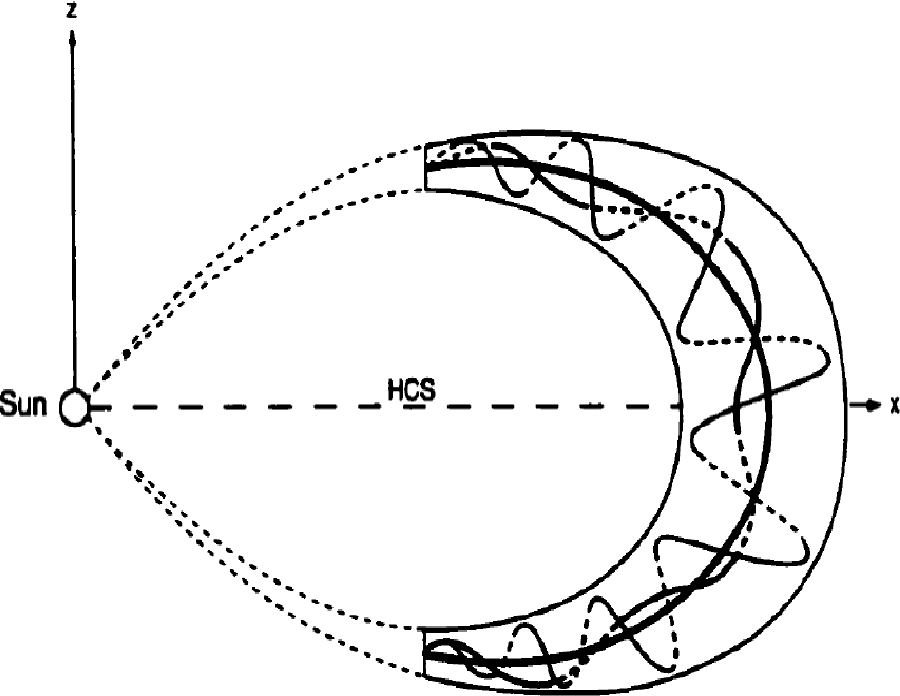
\includegraphics[width=0.75\textwidth]{Figures/fluxrope.png}
    \caption{Diagram of a magnetic cloud, with twisted magnetic field lines in a tube-like formation around a central axis \citep{Feng:2020}.}
    \label{fig:FR-diagram}
\end{figure}

In situ observations show that a continuous distribution of flux ropes sizes is present in the solar wind \citep{Feng:2007, Hu:2018}, but large-scale structures tend to be more easily identifiable and are better understood than small-scale flux ropes. Large-scale structures, also known as magnetic clouds, originate from the sun as a subset of interplanetary coronal mass ejections, and as such have distinguishable features. SFRs have a more ambiguous origin, and typically exhibit spatial scales $\lesssim$ 0.01 AU and time scales from less than a few minutes to a few hours based on in situ spacecraft measurements and analysis in the solar wind near Earth \citep{Cartwright:2010, Feng:2007, Hu:2018}. Figure \ref{fig:SFR-sizes} shows the distributions of duration and scale size of SFRs, grouped by heliocentric radial distances between $\sim$0.3 and 0.99 AU, from \cite{ChenHu:2020}.

\begin{figure}
    \centering
    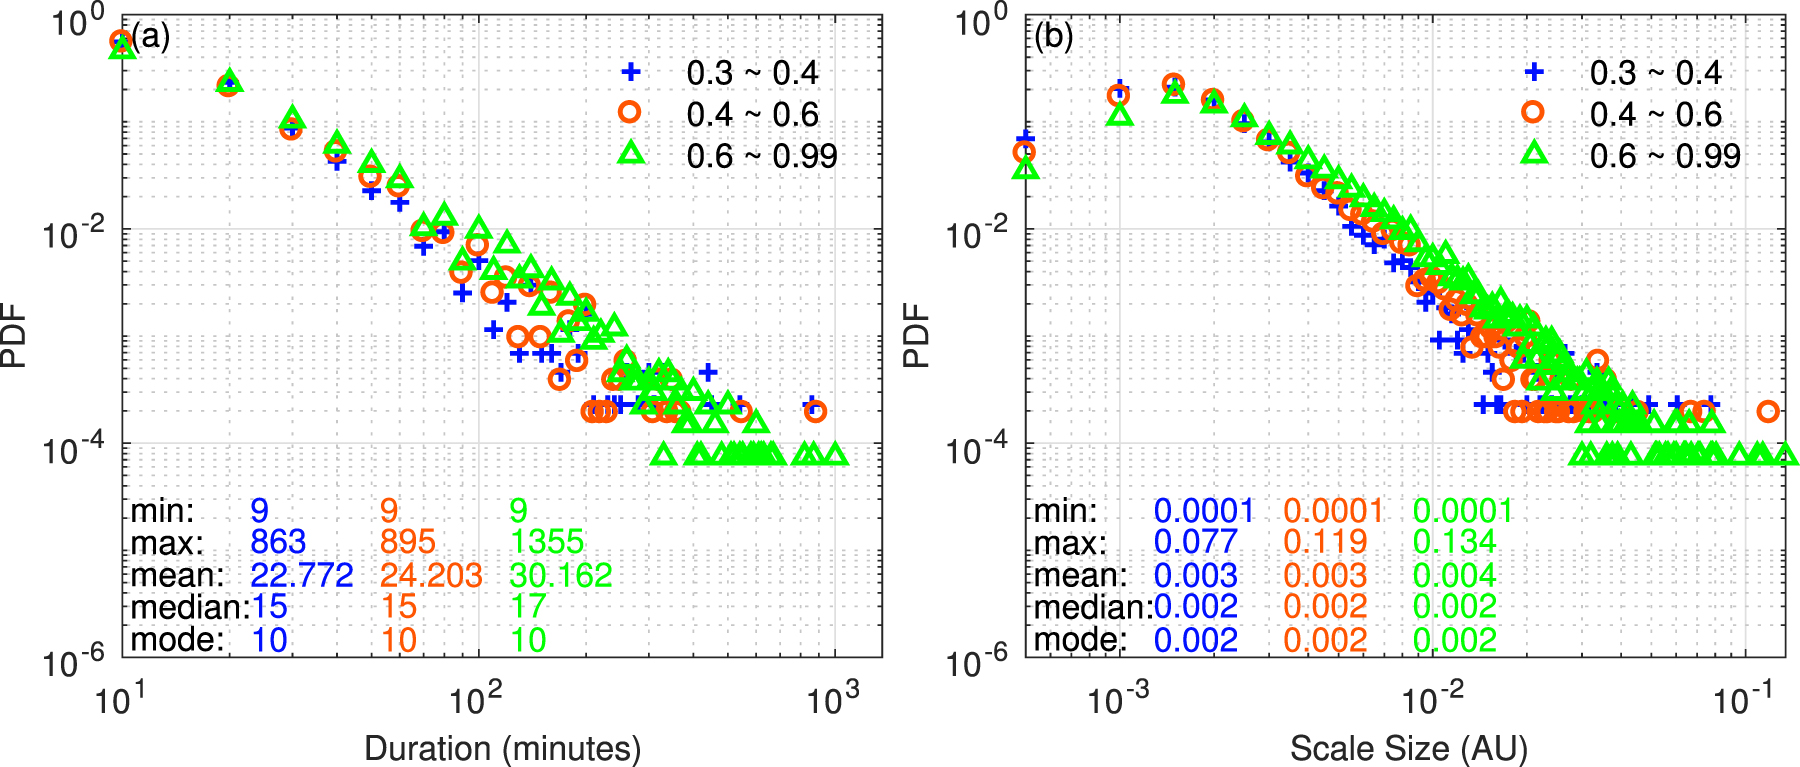
\includegraphics[width=\textwidth]{Figures/helios_Chen21.jpg}
    \caption[Distributions of scale-size of SFRs from Helios 1 and 2 \citep{ChenHu:2020}]{Distributions of (a) duration and (b) scale size of SFRs from Helios 1 and 2, grouped by radial distances from \cite{ChenHu:2020}.}
    \label{fig:SFR-sizes}
\end{figure}

\subsection{Alfv\'enic structures}
This twisted magnetic field topology is not unique to static flux rope structures in the interplanetary medium. Static SFRs are convected with the solar wind \citep{Cartwright:2008}. Alfv\'enic structures have similar magnetic field topology as flux ropes, but they propagate in the direction of the magnetic field. Alfv\'en waves are electromagnetic waves in which ions oscillate along a magnetic field line at the Alfv\'en speed. The restorative force comes from background magnetic field providing an effective tension while the inertia comes from the mass of the ions \citep{Alfven:1942}. These structures have significant field-aligned (parallel or anti-parallel) flow, which is characterized by Alfv\'enicity, the alignment between the velocity and magnetic field components. The Alfv\'enicity of a structure can be evaluated with the Wal\'en test, a linear regression between the remaining flow, $\mathbf{V_{sw}} - \mathbf{V_{HT}}$, and the Alfv\'en velocity $\mathbf{V_A}$. The physical properties of a moving structure are best evaluated in the co-moving frame, for which the de Hoffmann-Teller frame \citep{deHoffman-Teller:1950} is the simplest to apply. Thus, we subtract the de Hoffmann-Teller velocity $\mathbf{V_{HT}}$ from the bulk flow velocity $\mathbf{V_{sw}}$ in order to evaluate the field-aligned flow in magnetic structures.

Like SFRs, the helical structure of Alfv\'enic structures leads to high levels of magnetic helicity $H_m$\footnotemark{}, a measure of twisted-ness of the field lines. Another quantity that can be used to distinguish static structures and Alfv\'enic structures is residual energy, $E_r$\footnotemark[\value{footnote}]\footnotetext{defined in Section \ref{sec:wavelet-algorithm}}, which characterizes the imbalance between magnetic and kinetic energy. Level of Alfv\'enicity, is also characterized by the correlation between velocity and magnetic field fluctuations which can be represented by cross helicity $H_c$\footnotemark[\value{footnote}]. Alfv\'enic structures are structures that exhibit high levels of Alfv\'enic characteristics. The latter two parameters have been widely adopted as a way to describe the degree of Alfv\'enicity based on time-series analysis. For Alfv\'enic structures, the absolute value of the normalized cross helicity $|\sigma_c|$ is close to 1, and the normalized residual energy $\sigma_r$ is close to 0. For pure Alfv\'en waves, these two quantities are suggested to be 1 and 0, respectively \citep{Bruno:2013}. Flux ropes in the traditional view are supposed to have low Alfv\'enicity, i.e, being static. Considering the crossing of the boundary between the solar wind and the magnetosheath, I adopt a broad definition of SFRs in this study, by including both quasi-static structures and those possessing significant field-aligned flows with modest to high levels of Alfv\'enicity \citep{Chen:2022}.

%\subsection{Current sheets}


\section{Objectives}
Previous studies of SFRs such as \cite{Chen:2022} have used the extended Grad-Shafranov (GS) based techniques for the solar wind plasma; however, this algorithm was not used in other regions of near-Earth space such as the magnetosheath. Furthermore, many studies regarding flux ropes and other magnetic structures \citep{Zhao:2020, Chen:2021} focus on events identified during specific periods of time, instead of using multiple spacecraft for a coordinated study in the regions immediately upstream and downstream of the bow shock. In this study, I seek to identify magnetic structures via both the wavelet analysis and the extended GS-based algorithm in a systematic manner. This work characterizes magnetic structures with varying degrees of Alfv\'enicity as they move across boundaries in near-Earth space, and describe the characteristics and changes that magnetic structures exhibit as they occur in the solar wind and the magnetosheath, respectively.  

The identification and analysis of structures moving across boundaries such as the Earth's bow shock will give insight into how their properties change across this boundary as well as further our understanding of the interrelation between these structures. This study is observational and data-focused, with the specific goal to collect an inventory of events with high magnetic helicity. Another objective is to interpret and inter-compare the statistical properties of the structures, largely the SFRs, from the upstream solar wind and magnetosheath.

\chapter{Chapter 2. Data sets and pre-processing}\label{ch:ch2_data}

The data in this study are time series measurements from the Time History of Events and Macroscale Interactions during Substorms-Acceleration, Reconnection, Turbulence and Electrodynamics of the Moon’s Interaction with the Sun (THEMIS-ARTEMIS) mission and the Magnetospheric Multiscale (MMS) mission. The former mission seeks to investigate substorms in the Earth's magnetosphere, observe the Earth's radiation belts, and examine solar wind-magnetosphere interaction on the day-side. 


\section{THEMIS data set}
The THEMIS spacecraft are optimized for observing different regions of the magnetosphere and near-Earth solar wind. The five THEMIS probes (THM A-E) are traversing near-Earth space in different regions and orbits according to the science phases. THEMIS-B and THEMIS-C were reassigned as ARTEMIS-P1 and ARTEMIS-P2, respectively, in 2009 to facilitate observations at lunar Lagrange points 1 and 2. The separation between the probes, specifically during the mission phases in which simultaneous observation between the solar wind and magnetosheath are available, makes this mission ideal for use in this study.

Aboard each of the five THEMIS probes, identical Electrostatic Analyzer (ESA) instruments measure ion and electron distribution functions in three dimensions via spherical top-hat electrostatic analyzers \citep{McFadden:2008}. The observable range of energy fluxes of the ESA instrument is approximately 1.6-25 keV for ions and 2-32 keV for electrons. The Fluxgate Magnetometers (FGM) on each THEMIS probe \citep{Auster:2008} are single digital fluxgate magnetometers with a sensor at the end of a 2 meter boom. Because of the mission goals related to magnetic reconnection during substorms, the fluxgate magnetometers are very sensitive, with precision down to 0.1 nT, and operate in the range of 0.1-25000 nT \citep{Auster:2008}. Figure \ref{fig:thm-diagram} displays the arrangement of the instruments on a singular THEMIS probe. The FGM is located on the end of the boom, with the ESA and other instruments placed around the body of the spacecraft.

\begin{figure}
    \centering
    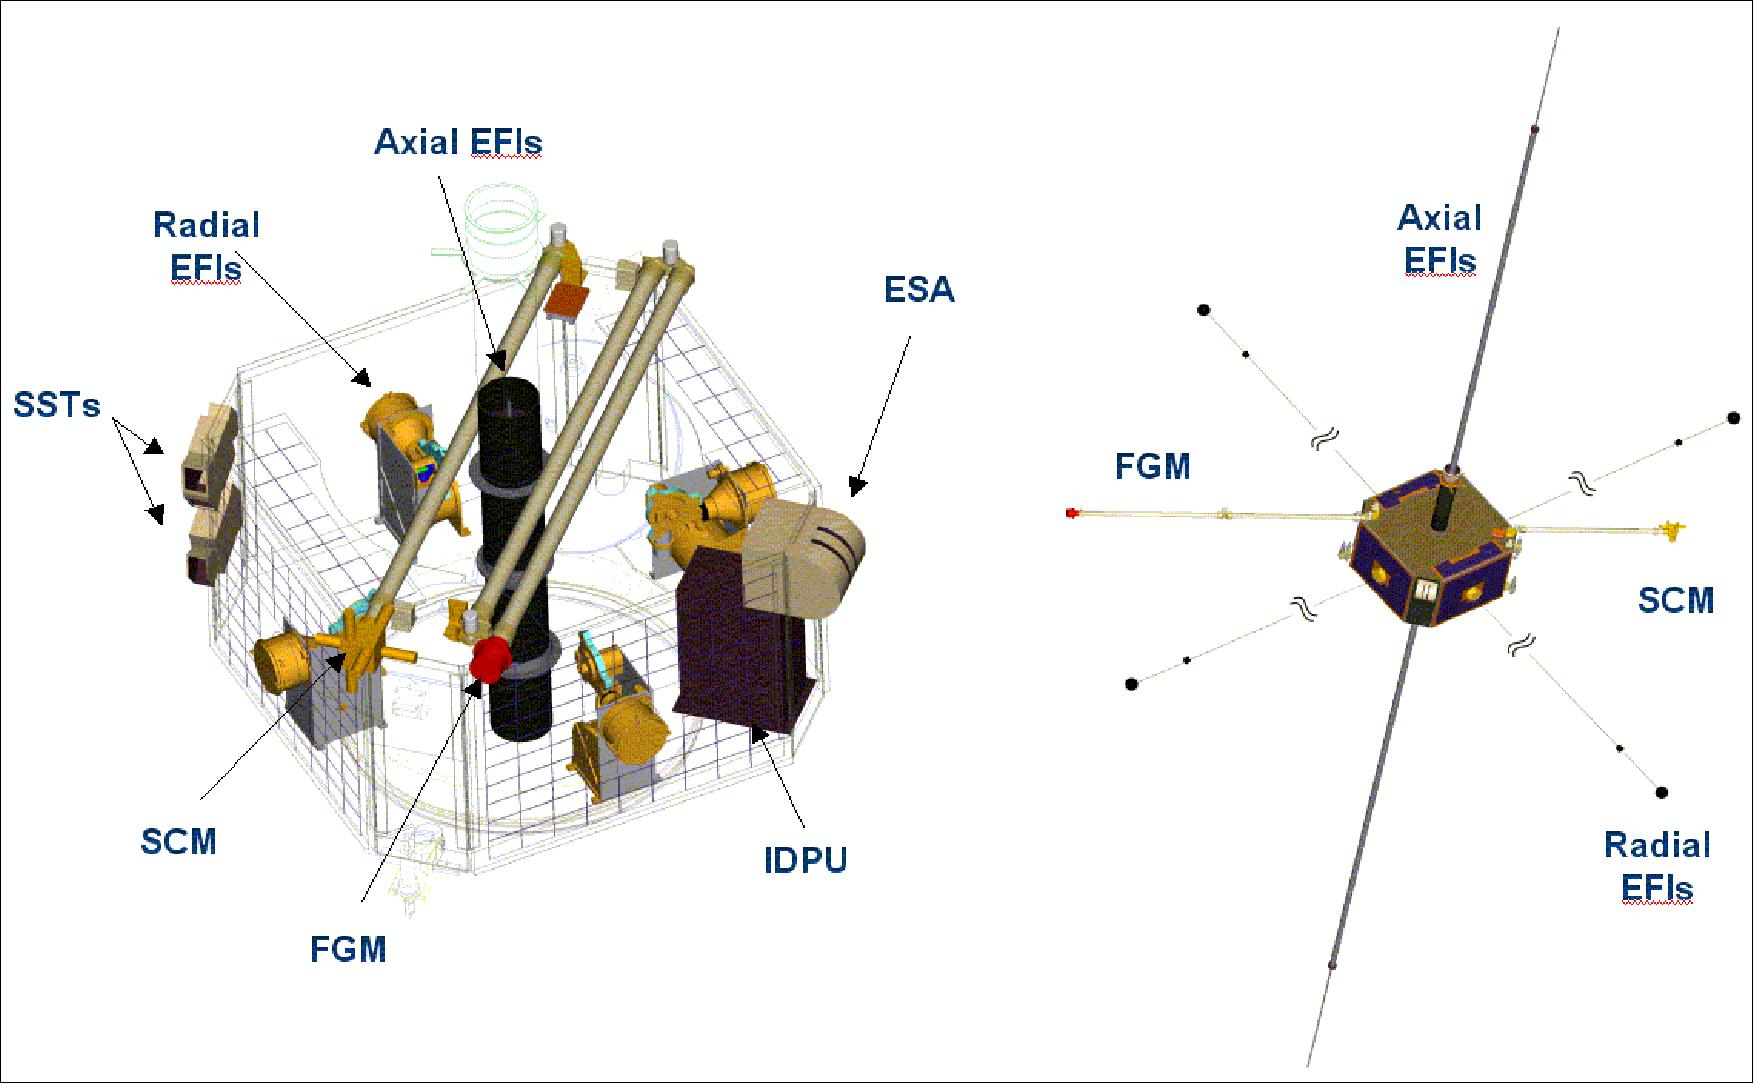
\includegraphics[width=\textwidth]{Figures/Instrumentation/THM_diagram.jpeg}
    \caption[Configuration of instruments on a singular THEMIS probe]{Configuration of instruments on a singular THEMIS probe. On the left, all of the instruments are shown, including the FGM and ESA. On the right, the Fluxgate Magnetometer (FGM) can be seen at the end of its 2 meter long boom, along with the Search Coil magnetomter (SCM) and Electric Field Instrument (EFI) \citep{eoPortal}.}
    \label{fig:thm-diagram}
\end{figure}

\section{MMS data set}
The MMS mission, comprised of four identical probes in a tetrahedral formation, also moves through the solar wind and magnetosheath. The magnetic field data from MMS come from the Fluxgate Magnetometer (FGM), which is part of the FIELDS suite on MMS \citep{Torbert:2016}. The MMS FIELDS suite is responsible for measuring the magnetic and electric fields. The FGM is comprised of two magnetometers on each spacecraft, one analog (AFG) and one digital (DFG). The magnetometers measure the magnetic field components with three-axis sensors \citep{Torbert:2016}. The two magnetometers are located on opposite sides of the spacecraft, each at the end of a five meter long boom (see Figure \ref{fig:fgm-mms}). Because there are two magnetometers on each spacecraft, they provide redundant data which is used to cross-calibrate the AFG and DFG instruments \citep{Torbert:2016}. The other instruments of the FIELDS suite are the Search Coil Magnetometer (SCM), which measures the magnetic field fluctuations over 1 Hz-6 kHz. The Spin-plane Double-Probes (SDP) and the Axial Double Probe (ADP) measure the electric field in the spin plane and along the spin axis, respectively. The Electron Drift Instrument measures ambient electron flux, and the EDI is used to conduct geometric measurements of the electric field and time-of-flight measurements for the magnetic field.
% determination of the offsets in the spin axis component of the AFG and DFG

\begin{figure}
    \centering
    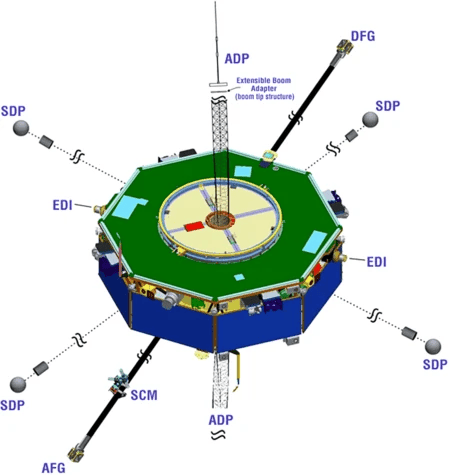
\includegraphics[width=0.7\textwidth]{Figures/Instrumentation/Torbert_Figure7.png}
    \caption[MMS FIELDS suite]{The MMS FIELDS suite on an individual probe, which measures magnetic and electric fields. The analog fluxgate magnetometer (AFG) and digital fluxgate magnetometer (DFG) are located at the ends of the two five meter booms, in the bottom left corner and top right corner. The Search Coil Magnetometer (SCM),  Electron Drift Instrument (EDI), Spin-plane Double-Probes (SDP), and the Axial Double-Probes (ADP) complete the FIELDS suite aboard each MMS spacecraft \citep{Burch:2024}.}
    \label{fig:fgm-mms}
\end{figure}

The Fast Plasma Investigation (FPI) \citep{Pollock:2016} instrument on MMS measures the velocity-space distribution of ions and electrons in the plasma in near-Earth space, from which their energy and velocity can be ascertained. Four dual electron spectrometers (DES) and four dual ion spectrometers (DIS) are evenly placed around each of the four probes, which are then connected to individual (IDPU) and central (CDPU) data processing units \citep{Pollock:2016}. The spectrometers measure the energy of the ions and electrons from 10 eV to 30 keV by measuring their differential directional flux distributions at a time resolution of 150 ms (for ions) and 30 ms (for electrons). Figure \ref{fig:fpi-mms} displays the layout of the FPI spectrometers aboard each MMS spacecraft.

% \begin{figure}
%     \centering
%     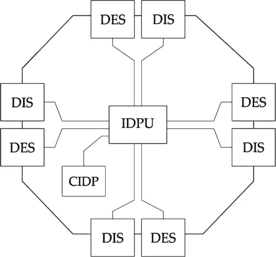
\includegraphics[width=0.7\textwidth]{Figures//Instrumentation/Torbert_Figure4.png}
%     \caption[Schematic of DIS and DES instruments aboard MMS]{Schematic of the ion (DIS) and electron (DES) spectrometers, which shows how the instruments are connected to the individual instrument data processing unit (IDPU), which in turn is connected to the central data processing unit (CDPU) \citep{Pollock:2016}.} 
%     \label{fig:fpi-mms-schematic}
% \end{figure}

\begin{figure}
    \centering
    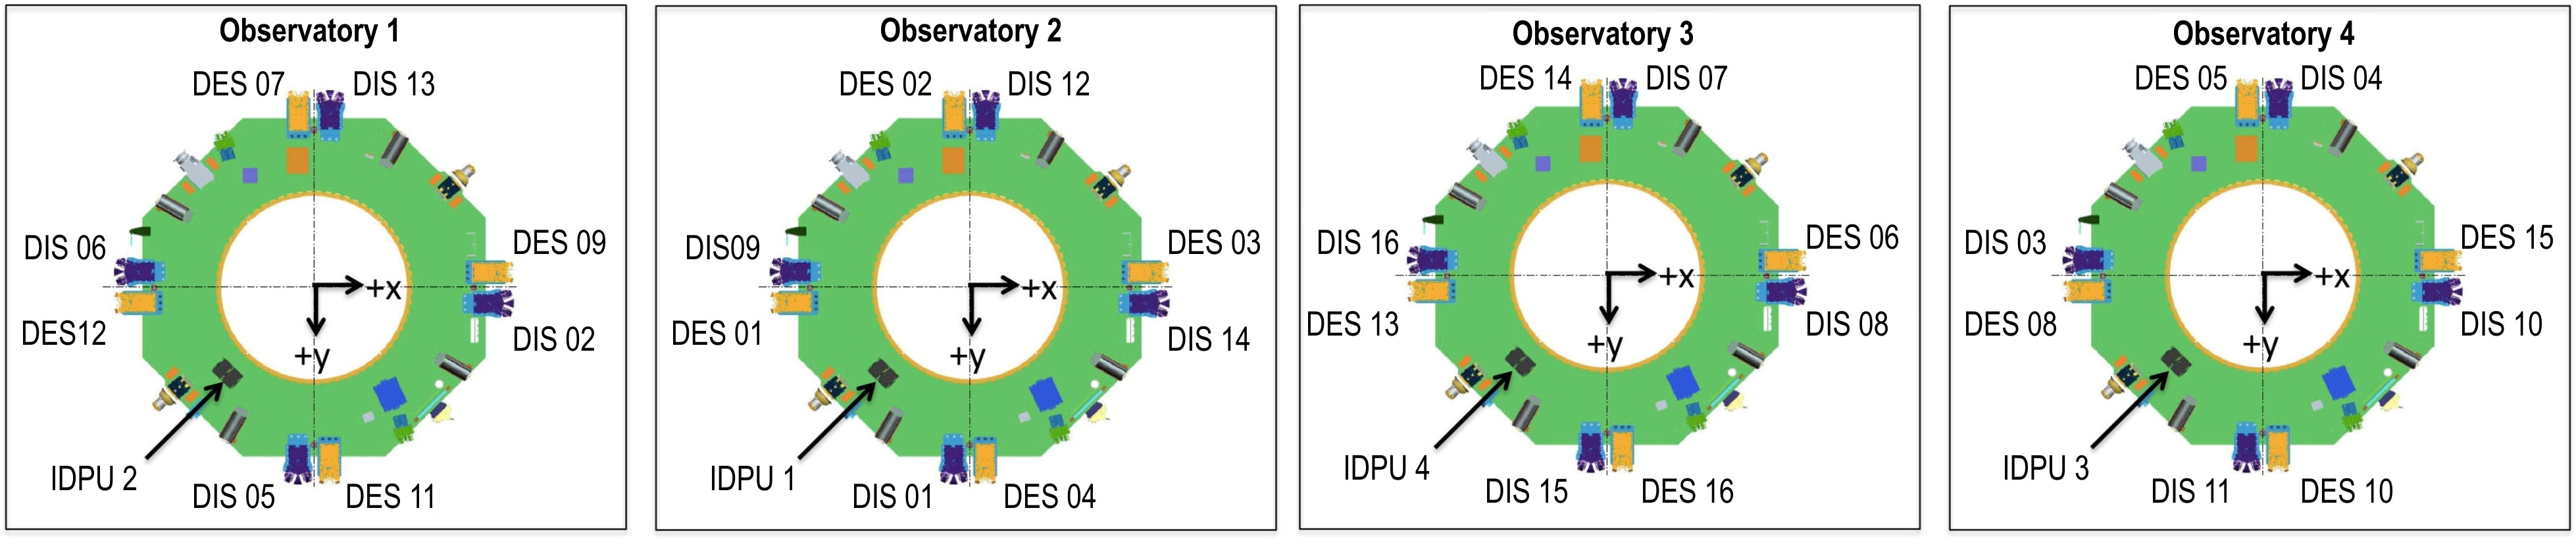
\includegraphics[width=\textwidth]{Figures//Instrumentation/Pollock_Figure5.jpg}
    \caption[MMS FPI instrument suite]{Diagram showing the full FPI instrument suite across each of the MMS spacecraft \citep{Pollock:2016}.}
    \label{fig:fpi-mms}
\end{figure}

\begin{figure}
    \centering
    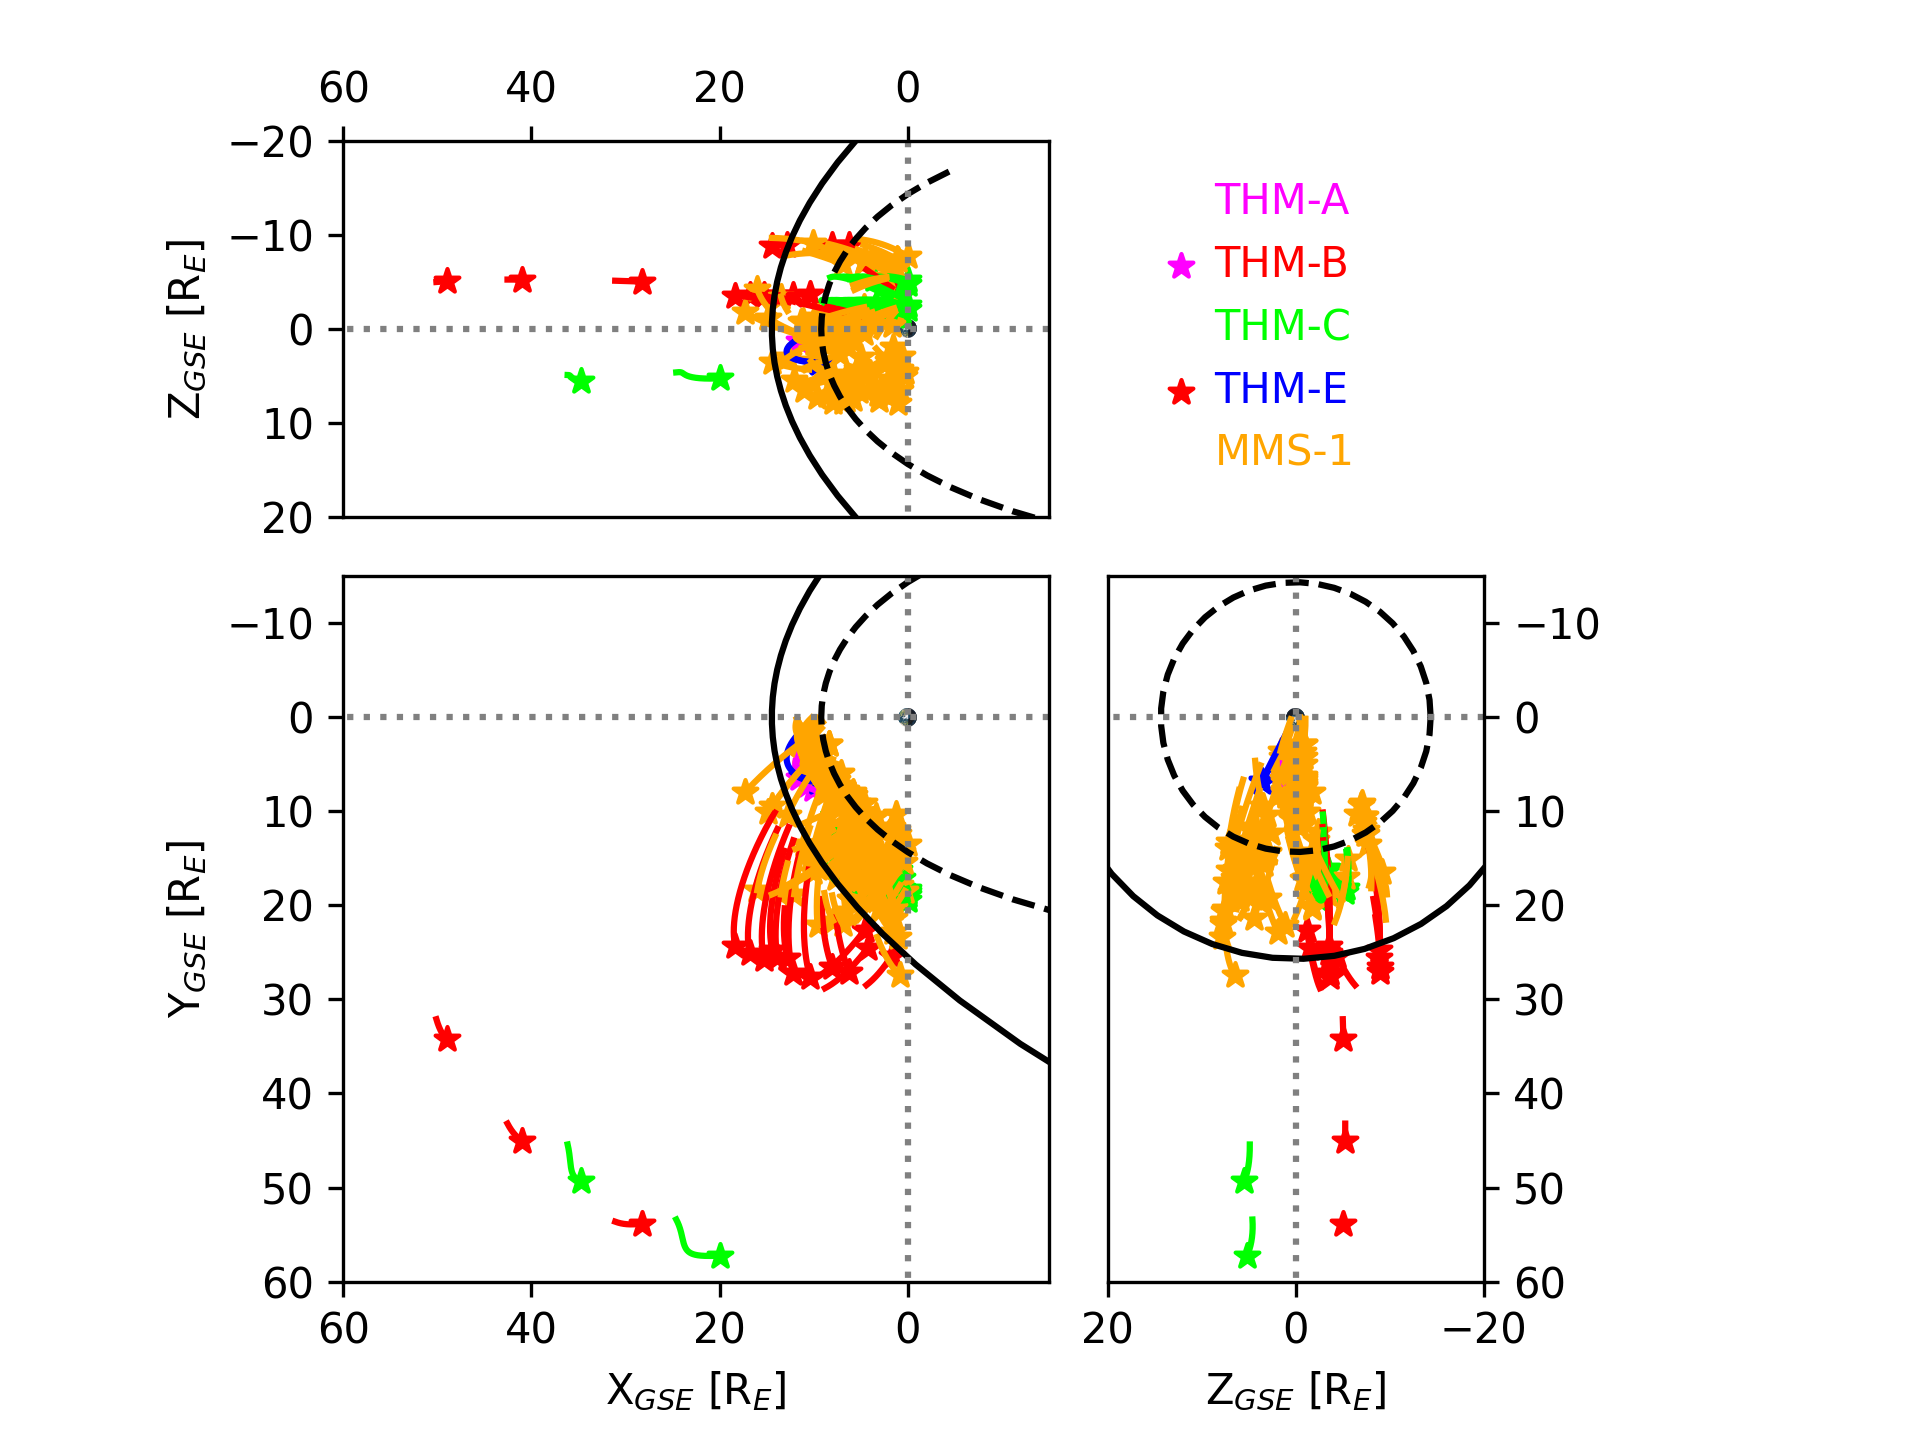
\includegraphics[width=\textwidth]{Figures/Orbits/all_TE_orbits_xy_xz_yz.png}
    \caption[Orbits for all observation periods]{Orbits for all analysis time periods are shown in the Geocentric Solar Ecliptic (GSE) coordinates for THEMIS probes A, B, C, and E (THM-A, THM-B, THM-C, THM-E) and MMS-1 probe (see legend), with the stars marking the end of each orbit period. The approximate nominal locations of the magnetopause (dashed black line) modeled using the \cite{Shue:1997} model and bow shock (solid black line) modeled using \cite{SlavinHolzer:1984} are shown, based on the IMF data obtained for one period in 2015 only.}
    \label{fig:all-orbits-plot}
\end{figure}

\section{Selection and pre-processing}
Hours-long periods of THEMIS data with cadence $\Delta t\sim$3 seconds and MMS data with $\Delta t=4.5$ seconds in the magnetosheath and near-Earth solar wind are chosen such that each analysis interval is entirely contained in one region to avoid transition regions. Figure \ref{fig:all-orbits-plot} shows the orbit segments of the THEMIS and MMS-1 probes for the selected time periods. The orange orbit lines display portions of the MMS-1 orbits from 2015-2023. The pink, red, green, and blue orbit lines show the THEMIS orbits in 2008, 2009, 2018, and 2022. The solid curve and dashed curve are the estimated bow shock and magnetopause boundaries \citep{SlavinHolzer:1984,Shue:1997}. These time periods, ranging in lengths from approximately 6 hours to 26 hours, are identified by looking at time series data and finding data segments bounded by simultaneous changes in magnetic field, plasma density, velocity, and ion spectra. Short instances of possible bow shock crossings (including multiple crossings) are identified in certain time periods, and the events identified in these crossing periods are removed from the final lists.

Figures \ref{fig:timeseries-MMS-magnetosheath} and \ref{fig:timeseries-THM-magnetosheath} are examples of two observed time periods in the magnetosheath from MMS-1 and THM-C, respectively. Figure \ref{fig:timeseries-THM-solarwind} shows the same observation period as Figure \ref{fig:timeseries-THM-magnetosheath}, but in the solar wind as observed by THM-B. These figures show the time series of magnetic field, plasma velocity, proton density, temperature, and ion energy spectra, as well as calculated values such as Alfv\'en velocity and proton beta. These quantities are used in our analysis, and also to identify the region in which the spacecraft was located. During the 19-20 June 2009 time period, THM-C experienced a bow shock crossing, which is denoted by the grey-shaded interval in Figure \ref{fig:timeseries-THM-magnetosheath}. By looking at the time series data during the whole period, and identifying changes in the data such as magnetic field and ion spectra that were consistent with bow shock crossings \citep{Lalti:2022,Trotta:2022}, periods where the spacecraft were experiencing a bow shock crossing were identified. The events in the bow shock crossing periods are removed from the final event list.

\begin{figure}
    \centering
    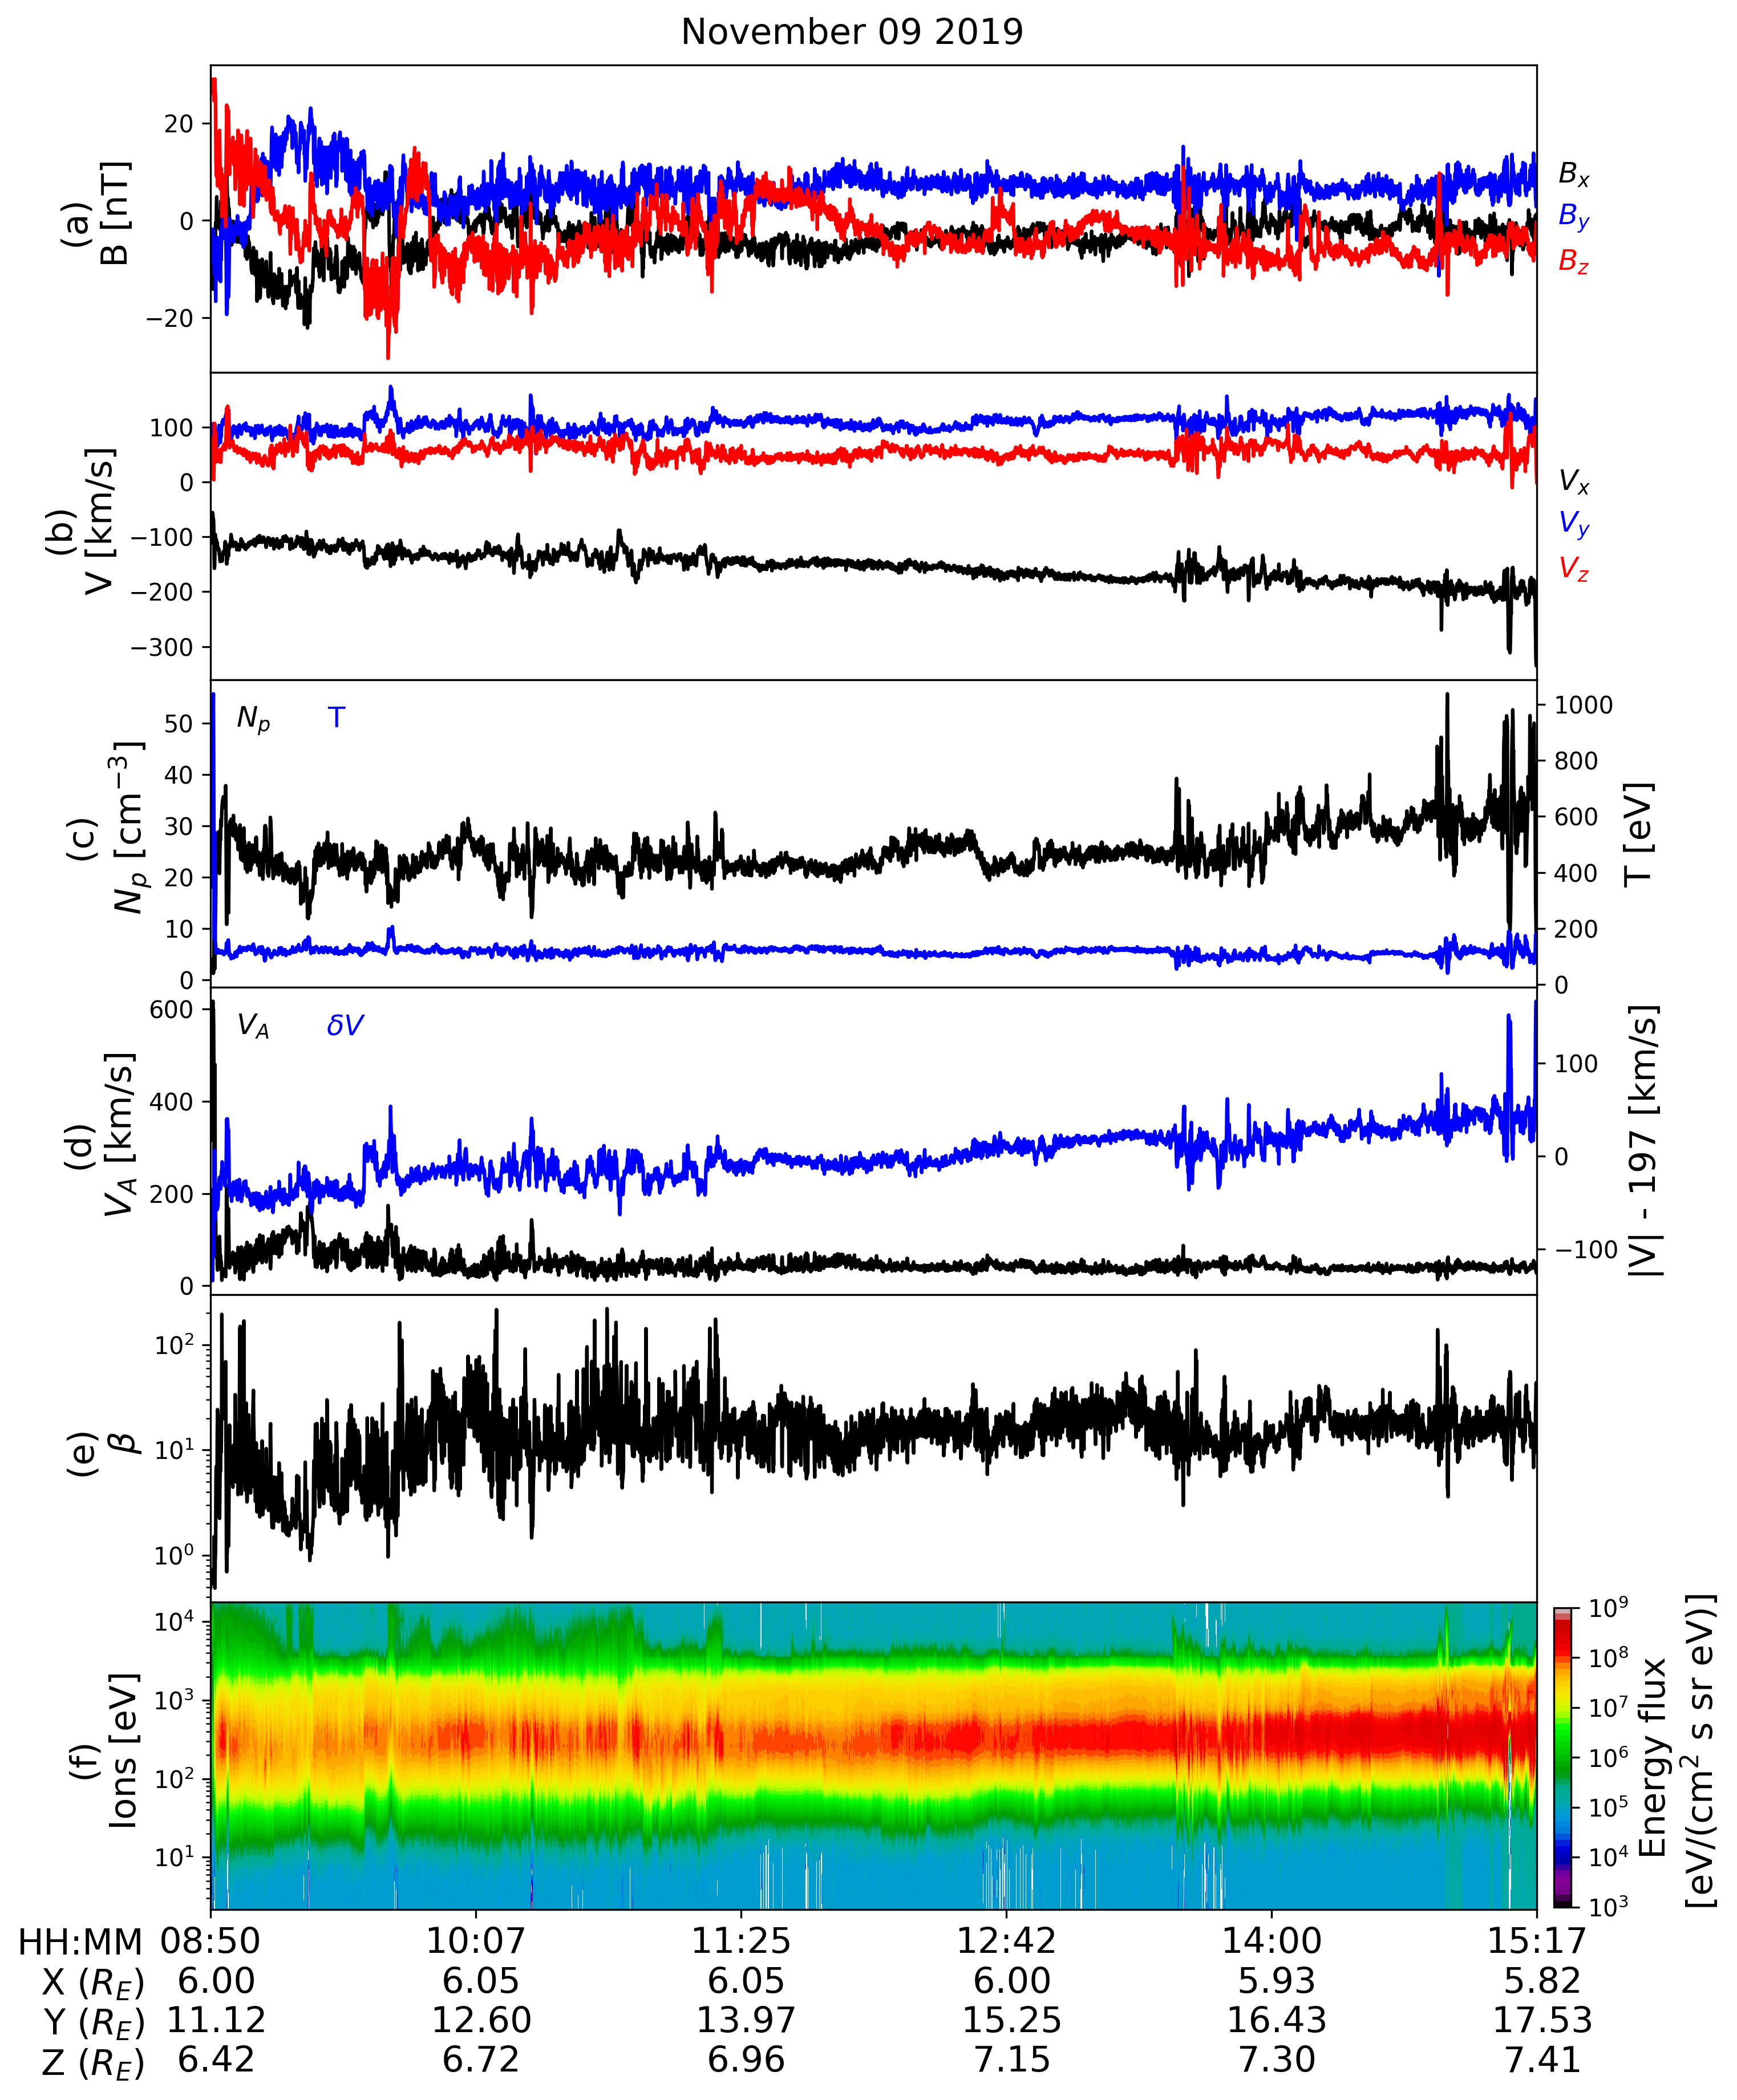
\includegraphics[width=0.9\textwidth]{Figures/Time series/timeseries_09112019_MMS1.png}
    \caption[Time series data observed in the magnetosheath on 9 November 2019]{Time series data observed by MMS-1 for $\sim$6 hours in the magnetosheath on 9 November 2019, with supplementary ephemeris data in GSE coordinates. The panels show a) magnetic field components, b) the components of flow velocity $\mathbf{V_{sw}}$, c) proton density and temperature, d) Alfv\'en speed and fluctuations of the magnitude of the velocity, e) proton beta, and f) ion spectra.}
    \label{fig:timeseries-MMS-magnetosheath}
\end{figure}

\begin{figure}
    \centering
    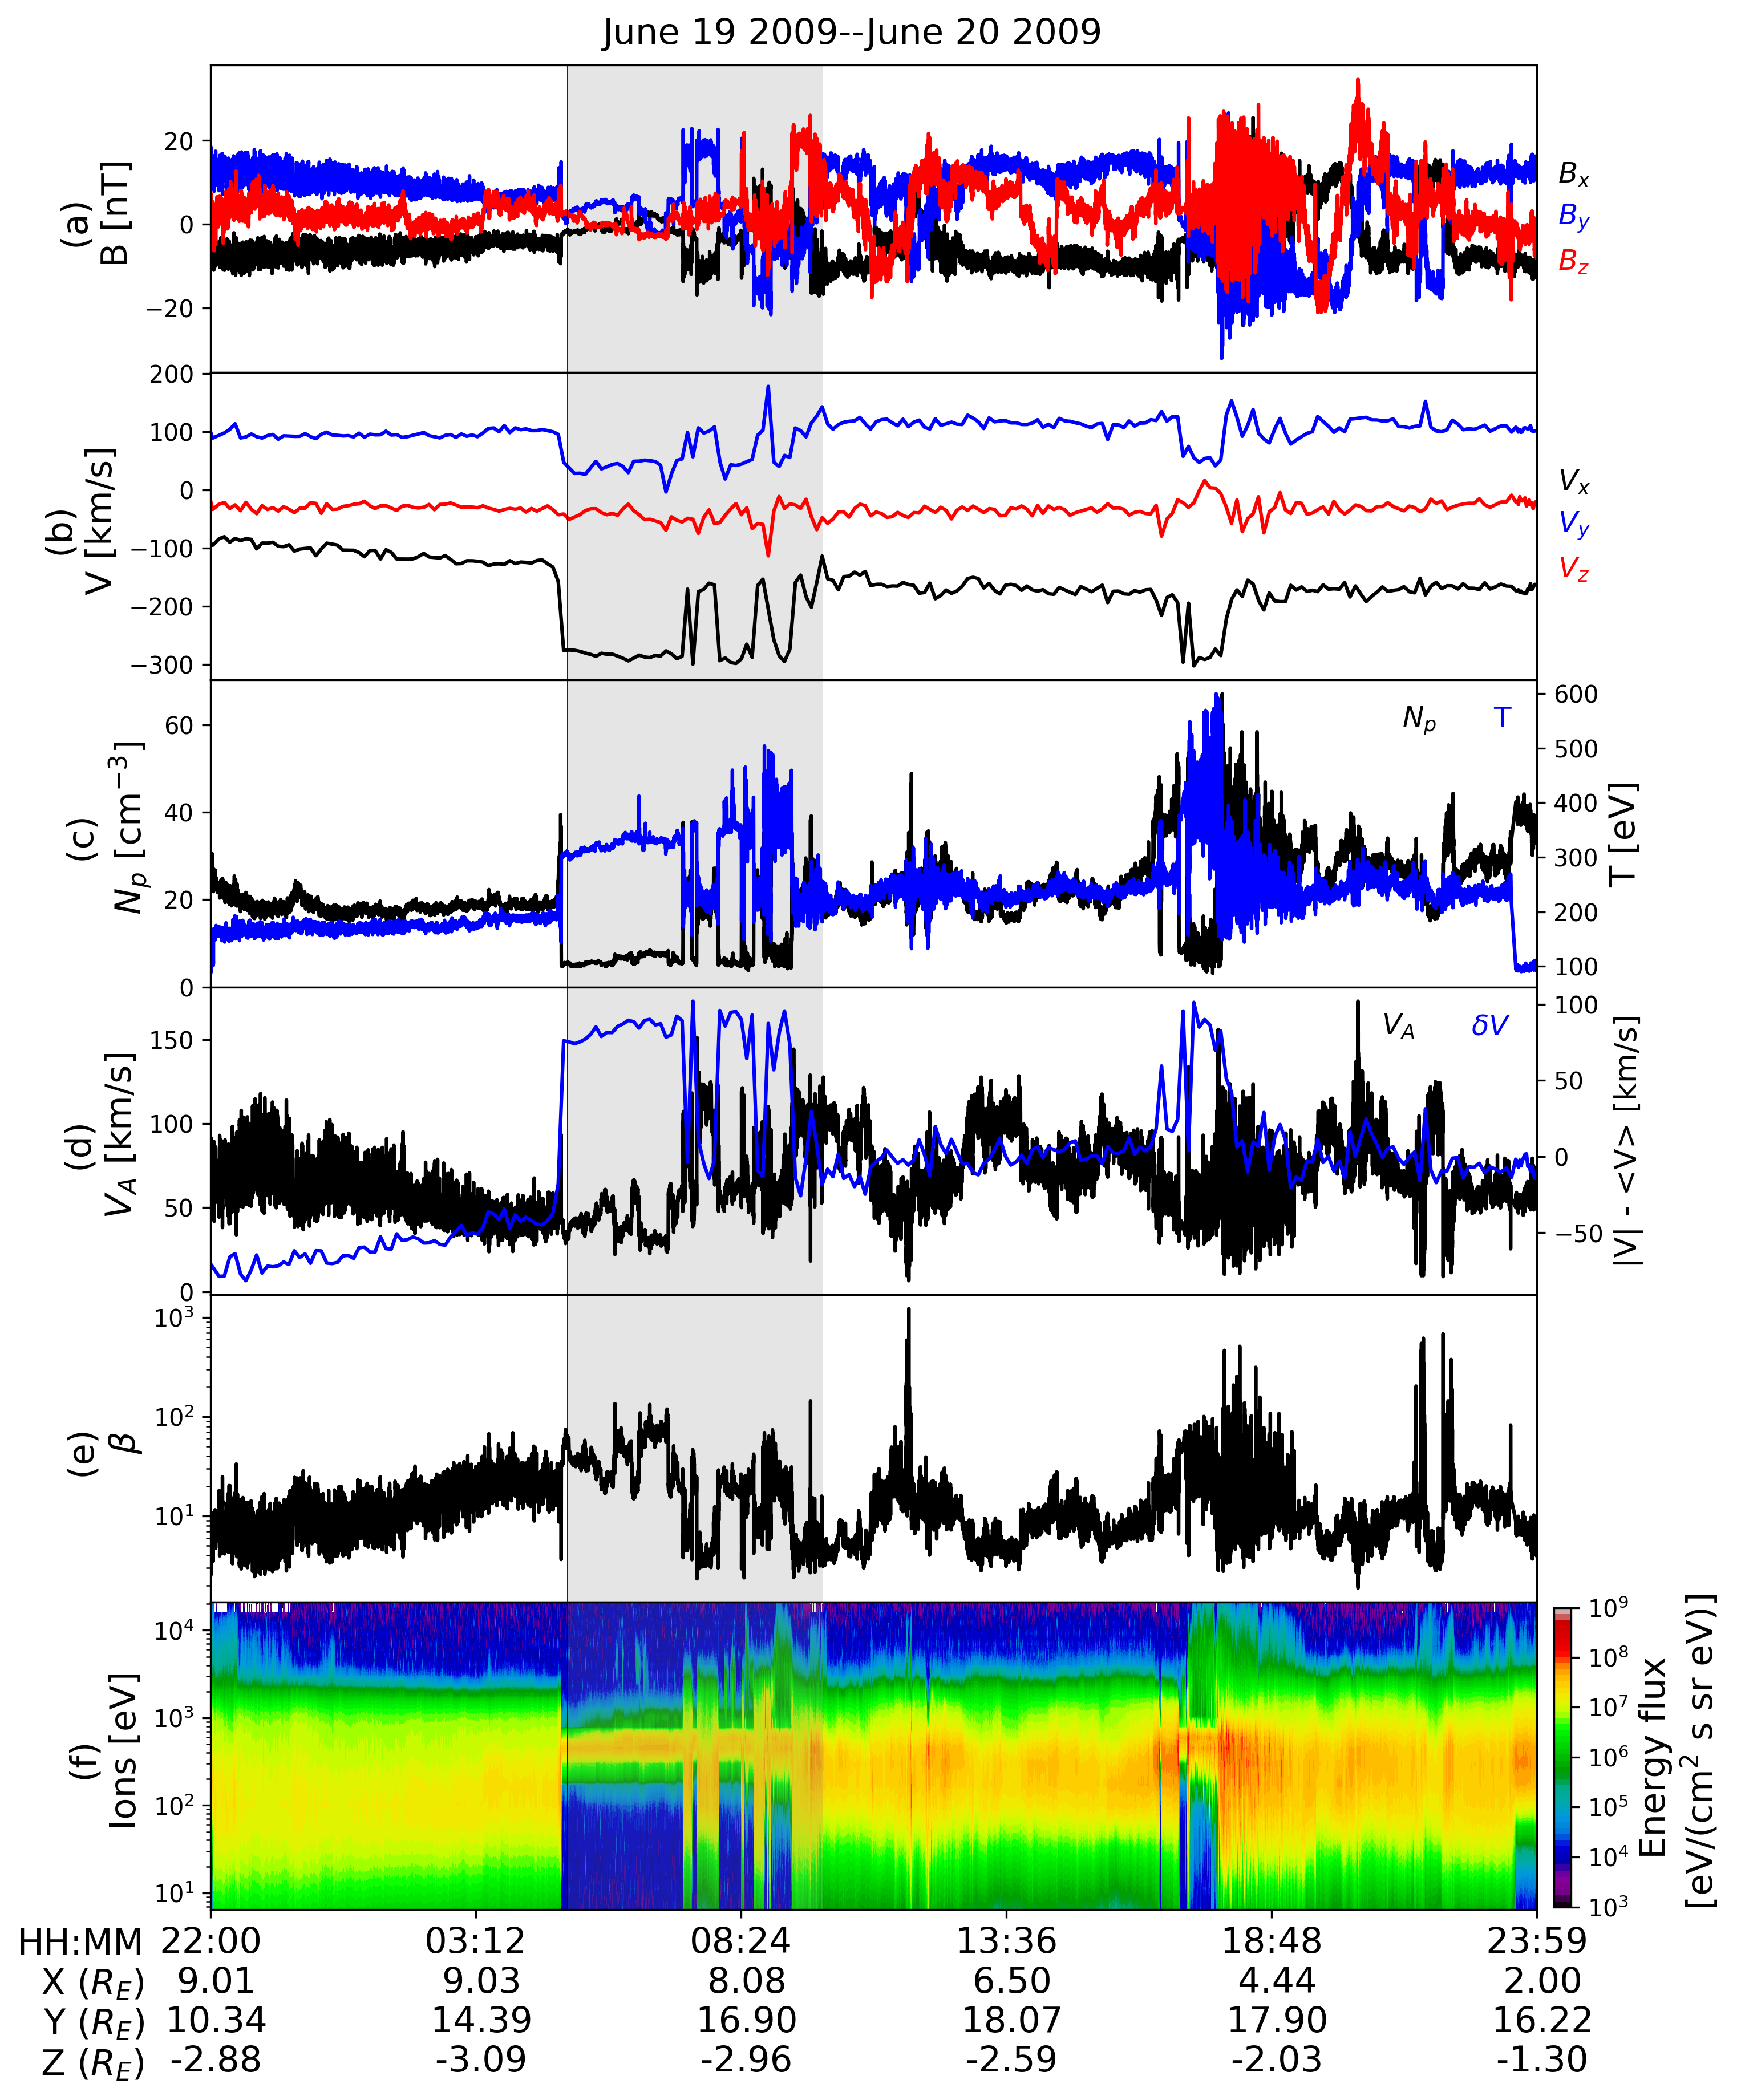
\includegraphics[width=0.9\textwidth]{Figures/Time series/timeseries_19062009_THMC.png}
    \caption[Time series data observed in the magnetosheath during 19-20 June 2009]{Time series data observed on 19-20 June 2009 by THM-C. This observation period spans $\sim$26 hours in the magnetosheath, with a bow shock crossing (grey region) identified during 5:00-10:00 UT on 20 June 2009. Similar to Figure \ref{fig:timeseries-MMS-magnetosheath}, the panels show the a) magnetic field, b) velocity, c) proton density and temperature, d) Alfv\'en speed and fluctuations of the magnitude of the velocity, e) proton beta, and f) ion spectra.}
    \label{fig:timeseries-THM-magnetosheath}
\end{figure}

\begin{figure}
    \centering
    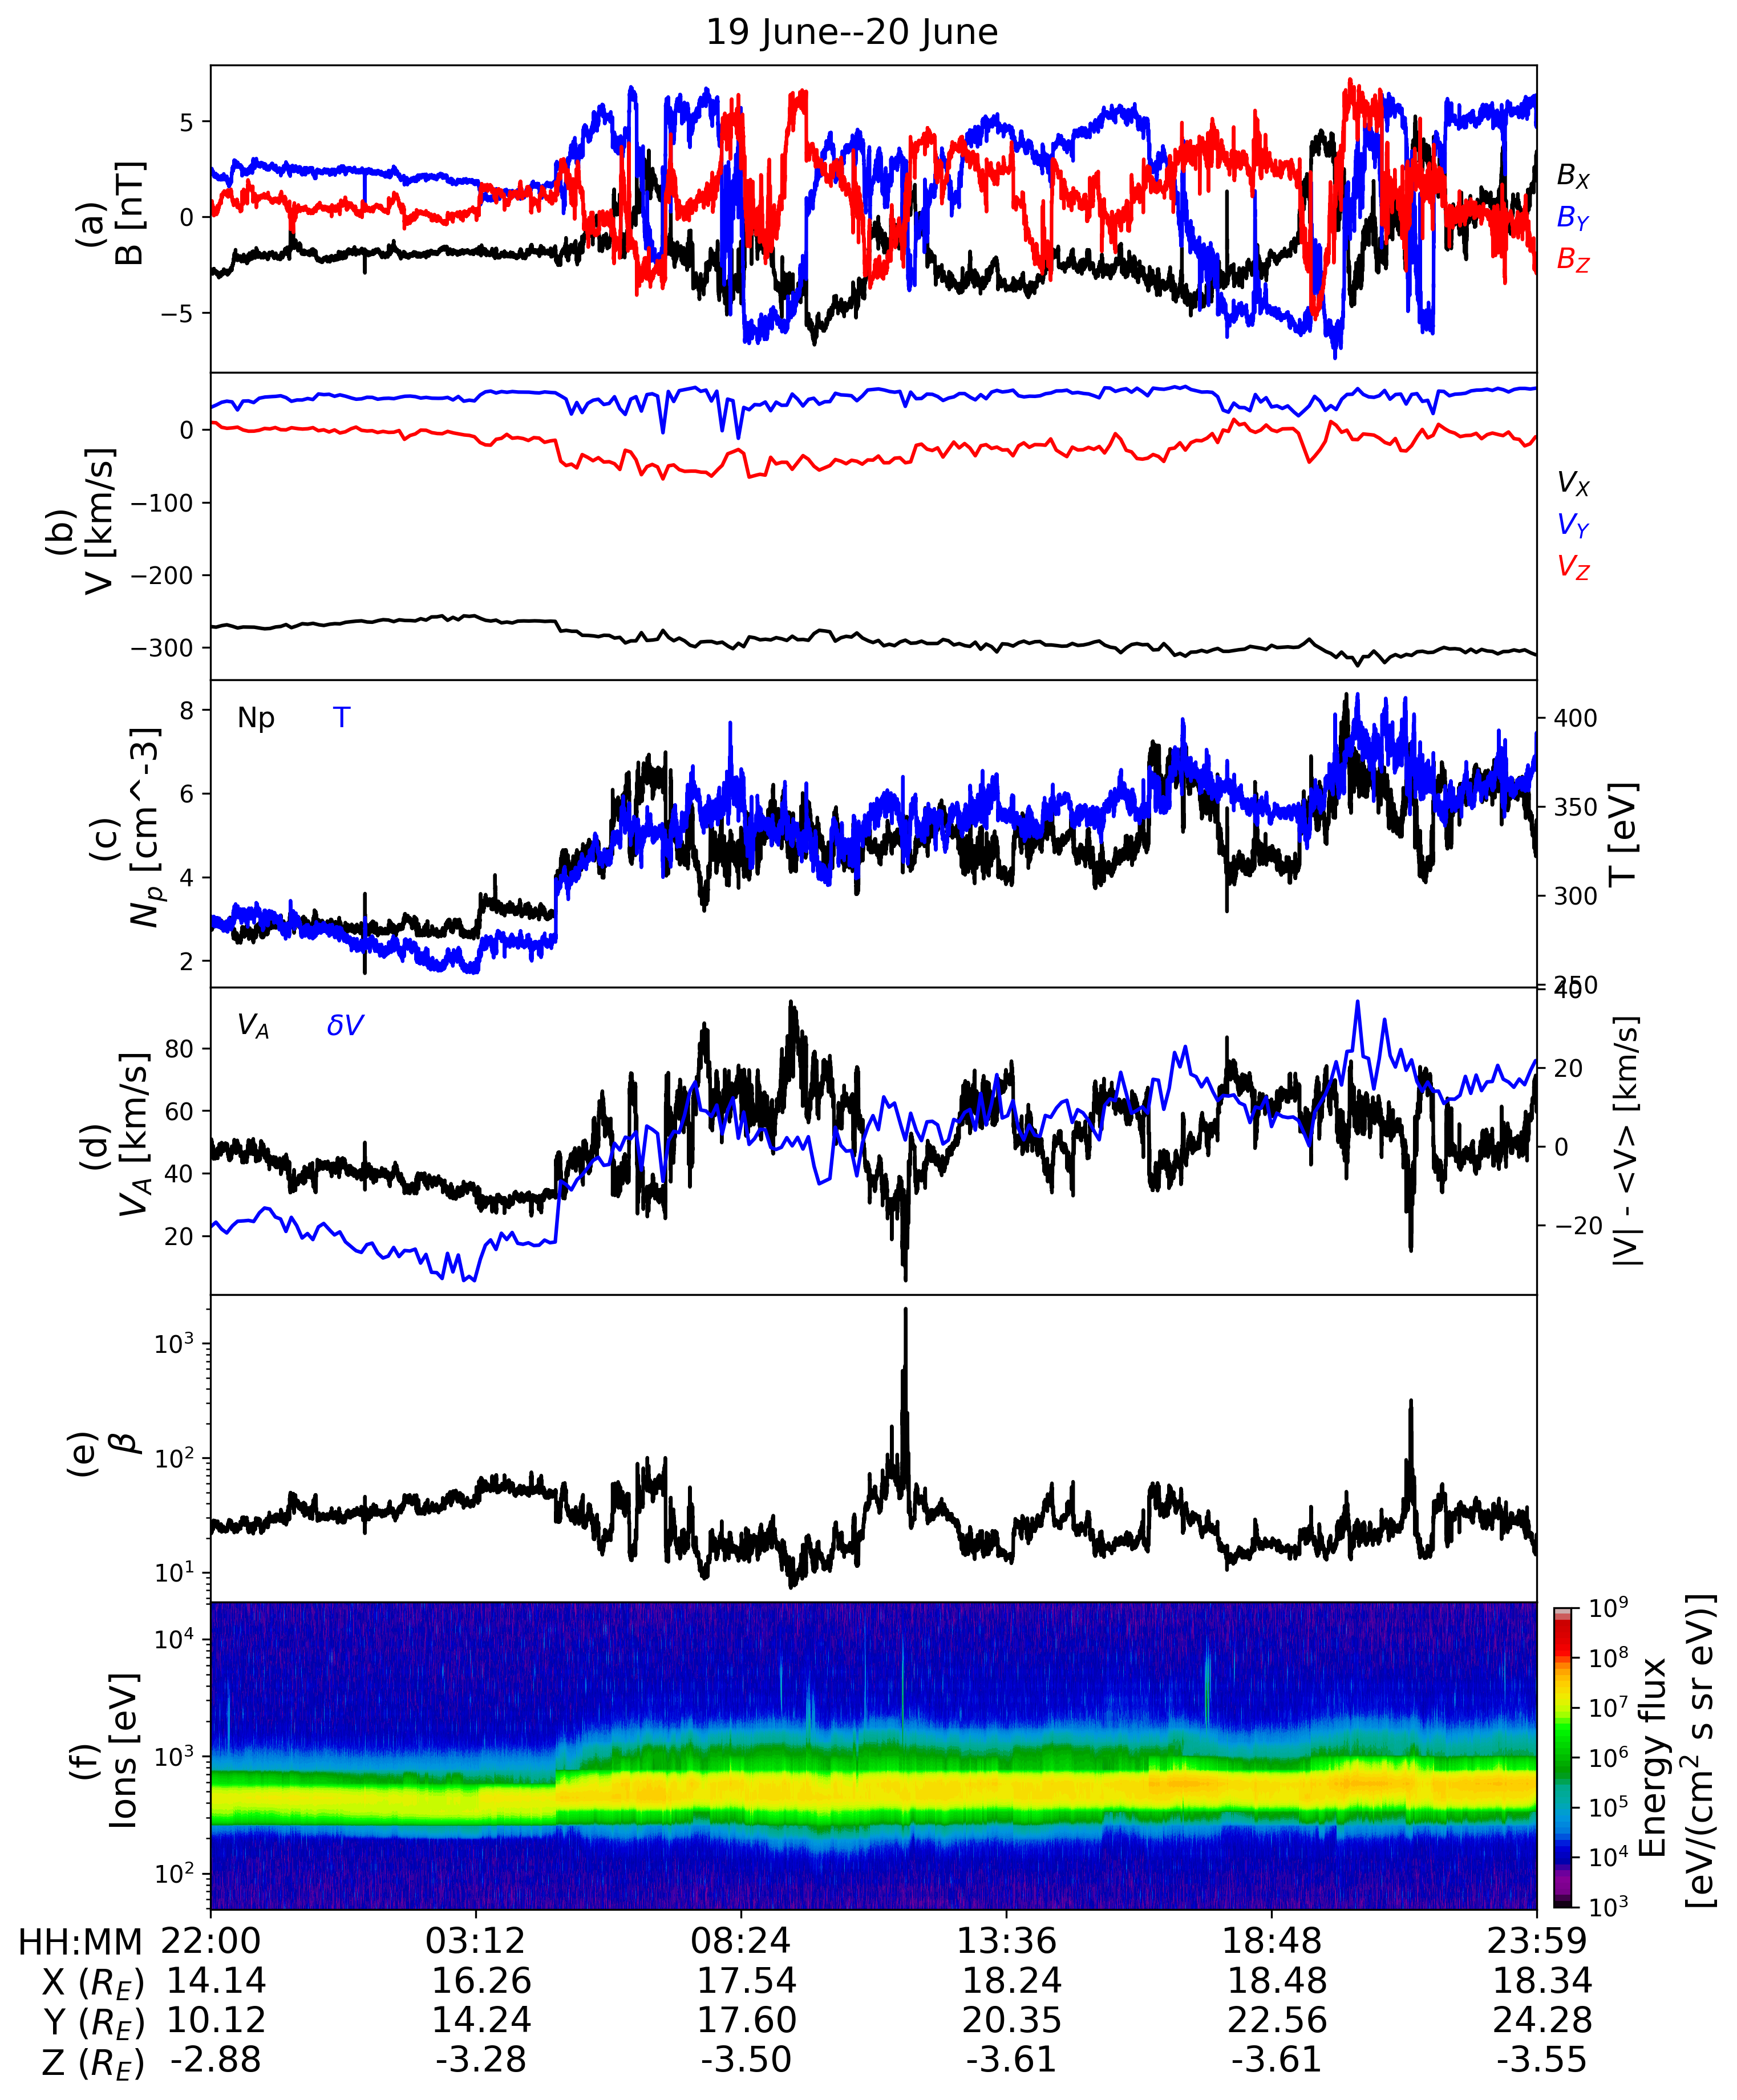
\includegraphics[width=0.9\textwidth]{Figures/Time series/timeseries_19062009_THMB.png}
    \caption[Time series data observed in the solar wind during 19-20 June 2009]{Time series data observed on 19-20 June 2009 by THM-B. This observation period spans $\sim$26 hours in the solar wind. Similar to Figure \ref{fig:timeseries-MMS-magnetosheath}, the panels show the a) magnetic field, b) velocity, c) proton density and temperature, d) Alfv\'en speed and fluctuations of the magnitude of the velocity, e) proton beta, and f) ion spectra.}
    \label{fig:timeseries-THM-solarwind}
\end{figure}

% Toy-Edens list
In addition to manually identifying periods in the solar wind and the magnetosheath, the published list of MMS data periods in the magnetosheath and solar wind from \cite{ToyEdens:2024} was also used. Their work focused on using unsupervised clustering to classify plasma regions in 8 years' worth of dayside MMS data \citep{ToyEdens2:2024}. The 1-minute resolution data was classified into the following regions: solar wind, ion foreshock, magnetosheath, and magnetosphere. The \cite{ToyEdens:2024} list contains over 9000 time periods in which MMS-1 to MMS-4 probes were identified to be solidly in the magnetosheath, with the minimum period being 15 minutes in length. The list of \cite{ToyEdens:2024} was refined by taking time periods with a duration longer than 5 hours for both the solar wind and magnetosheath regions, which is comparable to the shortest identified time period of THEMIS data. After further refining their magnetosheath list to the region downstream of the quasi-perpendicular bow shock (corresponding to a condition that the spacecraft location of $Y_{GSE}>0$), one-hundred and seven time periods were obtained to be used in this study. Fifty-eight periods, in which MMS traversed the solar wind upstream of the quasi-perpendicular bow shock, were obtained from the \cite{ToyEdens:2024} solar wind list. \cite{ToyEdens2:2024} include all MMS probes in their analysis; however, I only consider MMS-1 since presumably the other 3 MMS probes are in the same region, therefore I only report the results from MMS-1. In total, from the \cite{ToyEdens:2024} list and from our own identification, there were 130 time periods of data identified in the magnetosheath from THM-A, THM-C, THM-E, and MMS-1; and 77 periods identified in the solar wind from THM-B, THM-C, and MMS-1. The total lengths of the search time periods for our study are 1051 hours in the magnetosheath and 676 hours in the solar wind. A summary table of the observation search intervals can be found in Appendix \ref{appendix:observation-periods}. Table \ref{tab:data-products} displays the data products used in this work.

\begin{table}
    \centering
    \begin{tabular}{lcccc}
\hline
Data product            & Instrument & Symbol           & Units        & Cadence [s] \\
\hline
Magnetic field vector 	& FGM      & $B_X, B_Y, B_Z$  & nT                     & 2.74 - 4.295 \\
Flow velocity vector  	& ESA       & $V_X, V_Y, V_Z$  & km/s                  & 2.74 - 360$^a$ \\
Proton number density	& ESA       & $N_p$            	& cm$^{-3}$            & 2.74 - 4.295 \\
Proton temperature    	& ESA       & $T$            	& eV                   & 2.74 - 4.295 \\
Ion energy spectra    	& ESA       &                  	& eV/(cm$^2$ s sr eV)  & 2.74 - 4.295 \\
\hline
Magnetic field vector 	& FGM      & $B_X, B_Y, B_Z$  & nT                    & 4.5 \\
Flow velocity vector  	& FPI      & $V_X, V_Y, V_Z$  & km/s                  & 4.5 \\
Proton number density 	& FPI      & $N_p$            & cm$^{-3}$             & 4.5 \\
Proton temperature    	& FPI      & $T$              & eV                    & 4.5 \\
Ion energy spectra   	& FPI      &                  & eV/(cm$^2$ s sr eV)   & 4.5 \\
\hline
\end{tabular}
    \caption[Data products from THEMIS and MMS]{Data products from THEMIS (top) and MMS (bottom) used in this study. For the flow velocity vector from THEMIS, there are some periods in which 6-minute data was up-sampled to match the $\sim$ 3-second data.}
    \label{tab:data-products}
\end{table}

%A significant portion (green and red lines) of the coordinated analysis data periods are hidden behind the orange MMS orbit lines; however, the orbit plots for the coordinated analysis periods can be found in the appendix.

% note: 107 periods were used for detection; however of the total events, 5 events overlapped with mine that I had already run and then there was 1 period with data not available and 3 with time periods not really inside the magnetosheath by visual identification of time series data

\section*{Open Research}
The MMS and THEMIS data \citep{Torbert:2016,Pollock:2016} used in this study was retrieved from the NASA Science Data Center via the PySPEDAS software, which is open source and publicly available at \url{https://github.com/spedas/pyspedas} under an MIT license. The \cite{ToyEdens:2024} database of MMS periods in the solar wind and magnetosheath is available open access at \url{https://zenodo.org/records/11032322}, and the algorithm to generate this data is described in \cite{ToyEdens2:2024}.
\chapter{Chapter 3. Wavelet analysis as a single-spacecraft method}

Single-spacecraft measurements have been used in the identification of small-scale magnetic structures \citep{Pecora:2019, Telloni:2012, Hu:2018, Zheng:2018, Zhao:2020}. The time series data can be treated as a spatial snapshot due to the effective stationary state of the plasma medium traversed by a spacecraft relative to the fast-moving solar wind. Time series data are transformed directly to spatial distributions \citep{Taylor:1938}. Therefore, time-frequency transforms, such as wavelet transforms, are conceivably useful for analyzing features of in situ spacecraft time series at different frequencies over time \citep{Torrence:1998}. Specifically the power spectra associated with a number of selected MHD quantities are derived to characterize the underlying magnetic structures.

\section{Wavelet transforms}
Wavelet transforms are used to analyze time series with non-stationary power at different frequencies \citep{Torrence:1998} using non-orthogonal wavelet basis functions. Assuming a continuous signal as a function of time $t$, $x=x(t)$, the continuous wavelet transform is defined as
\begin{equation}
    W(s,\tau) = \frac{1}{|s|^{1/2}}\int_{-\infty}^\infty x(t)\psi^*\p{\frac{t-\tau}{s}}\textnormal{dt}.
    \label{eq:wavetrans}
\end{equation}
Here $\psi^*$ is the complex conjugate of the wavelet basis function $\psi(t)$, which is a function that must be localized in time and frequency space, and has zero mean \citep{Torrence:1998}.

As usual, with a discrete set of data points $x_n=x(t_n)$ with time resolution $\delta t$, the continuous wavelet transform takes the discrete form
\begin{equation}
    W_n(s,t) = \sum_{n'=0}^{N-1}x_{n'}\psi^*\pp{\frac{\p{n'-n}\delta t}{s}}.
    \label{eq:wavetrans2}
\end{equation}
In practice, discrete wavelet transforms are implemented for time series data by dilating the scale $s$ and translating along the time index $n$. This results in a two dimensional array of the wavelet transform. The scales are chosen such that
\begin{equation}
    J = \frac{\log_2\p{\frac{N \delta t}{s_0}}}{dj}
\end{equation}
\begin{equation}
    s_j = s_0 2^{j dj},\hspace{20pt} j = 0,...,J
    \label{eq:scales}
\end{equation}
where $s_0 = 2\delta t$ and the choice of $dj$ is sufficiently small for the width of the wavelet basis function in spectral space. The Morlet wavelet given in Equation (\ref{eq:morlet}) is a good wavelet base because it is complex and has good frequency resolution, thus it is frequently used in small-scale flux rope identification \citep{Telloni:2012, Telloni:2013, Zhao:2020, Farge:1992}:
\begin{equation}
    \psi_0(\eta) = \pi^{-1/4}e^{i\omega_0\eta}e^{-\eta^2/2}.
    \label{eq:morlet}
\end{equation}

Figure \ref{fig:wavelet-diagram} visually demonstrates the typical transform of a time series data set from the time domain to a time-frequency domain, including the Fourier transform and the wavelet transform. Wavelet transforms take a one-dimensional time series (top left corner of Figure \ref{fig:wavelet-diagram}) and transform it into a two-dimensional series (bottom right corner of Figure \ref{fig:wavelet-diagram}), whereas the Fourier transform applied to a one-dimensional time series yields a one-dimensional series in the frequency domain (top right corner of Figure \ref{fig:wavelet-diagram}). The Fourier transform decomposes a time series function into a combination of the frequencies present in the data set \citep{Farge:1992}. The Fourier transform of a time series $x(t)$ into its frequency domain (index $k$) is
\begin{equation}
    F(k) = \int_{-\infty}^\infty x(t) e^{-2\pi ikt/N} \textnormal{dt},
    \label{eq:fourier}
\end{equation}
\noindent and with discrete data $x_n = x(t_n)$, it takes the form
\begin{equation}
    F_n(k) = \frac{1}{N} \sum_{n=0}^{N-1}x_{n} e^{-2\pi ikn/N}.
    \label{eq:DFT}
\end{equation}
A short time Fourier transform (bottom left corner of Figure \ref{fig:wavelet-diagram}) can produce a two-dimensional time-frequency domain, but by segmenting the time series and performing a Fourier transform over the segments, the method only yields identical time-frequency domains, for each respective time segment. Fourier transforms theoretically retain all the `information' about an equation, but discrete Fourier transforms are a summation over a finite set and therefore are not as accurate. 

\begin{figure}
    \centering
    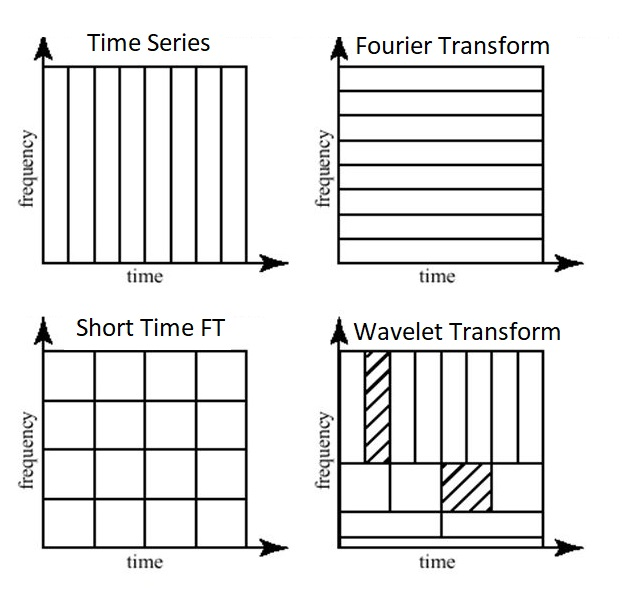
\includegraphics[width=0.7\textwidth]{Figures/Comparisonoftransformations.jpeg}
    \caption[Time and frequency resolutions of different transforms]{Time and frequency resolutions of different transforms applied to a one-dimensional time series dataset. The wavelet transform (bottom right) has non-uniform frequency and time resolution.}
    \label{fig:wavelet-diagram}
\end{figure}

% The calculation in (\ref{eq:wavetrans2}) can be more efficiently done in Fourier space. Using a discrete Fourier transform, all $N$ convolutions can be done simultaneously for each scale $s$. The discrete Fourier transforms of the time series $\xhat_k=x_n$ and $\psihat^*(s\omega_k)=\psi^*(s,t)$ are
% \eql{DFT}{\xhat_k = \frac{1}{N}\sum_{n=0}^{N-1}x_n e^{-2\pi ikn/N}}

% \eql{DFTpsi}{}

% By the convolution theorem, a wavelet transform is inverse Fourier transform of the product
% \eql{wavelet}{W_n(s,t) =\sum_{k=0}^{N-1} \xhat_k \psihat^*\p{s\omega_k} e^{i\omega_k n\delta t}}
% where

\section{MHD quantities}
The magnetic field lines in flux ropes are twisted such that they preside in a tube-like configuration. Thus, flux ropes carry magnetohydrodynamic (MHD) quantities such as cross helicity $H_c$ and magnetic helicity $H_m$, as well as residual energy $E_r$, defined as
\begin{equation}
    H_c = \frac{1}{2}\int \mathbf{v}\cdot\mathbf{b} \hspace{5pt} \mathrm{d^3} \mathbf{r}
    \label{eq:Hc}
\end{equation}
\begin{equation}
    H_m = \int \mathbf{A}\cdot\mathbf{B} \hspace{5pt} \mathrm{d^3} \mathbf{r}
    \label{eq:Hm}
\end{equation}
\begin{equation}
    E_r = \frac{1}{2} \pp{\pang{\mathbf{v}^2}  - \pang{\mathbf{b}^2}},
    \label{eq:Er}
\end{equation}
where $\mathbf{B}\p{\mathbf{x},t}$ is the magnetic field, $\mathbf{A}\p{\mathbf{x},t}$ is the magnetic vector potential, and $\mathbf{v}(\mathbf{x},t)$ and $\mathbf{b}(\mathbf{x},t)$ are the fluctuating velocity and magnetic field in Alfv\'en units. Cross helicity describes the measure of alignment between magnetic and velocity fluctuations, while magnetic helicity describes the “knottedness” of the magnetic field lines \citep{Matthaeus:1982}. High magnetic helicity is a signature of flux ropes, and often accompanied by low cross helicity \citep{Zhao:2020}. Residual energy describes the imbalance between magnetic and kinetic energy, and thus according to (\ref{eq:Er}), a negative residual energy will characterize an event with higher magnetic energy.
%When normalized, these magnetohydrodynamic quantities give insight into the nature of magnetic field structures, and allow us to identify these events in the solar wind and Earth's magnetosphere.

Normalized MHD quantities give insight into the nature of magnetic field structures, and allow us to identify and characterize these events. Approximated in the time domain, the normalized cross helicity and residual energy can be calculated using
\eql{eq:sigctime}{\sigma_c = \frac{2\langle\mathbf{v}\cdot\mathbf{b}\rangle}{\langle\mathbf{v}^2\rangle + \langle\mathbf{b}^2\rangle}}
\eql{eq:sigrtime}{\sigma_r = \frac{\langle\mathbf{v}^2\rangle - \langle\mathbf{b}^2\rangle}{\langle\mathbf{v}^2\rangle + \langle\mathbf{b}^2\rangle}}
where $\mathbf{v}$ is the remaining flow in the de Hoffman-Teller frame. Single spacecraft measurements cannot be used directly calculate reduced magnetic helicity, therefore other methods are required to approximate this quantity. The power spectral density of a time series describes the distribution of the energy across the frequency components of a signal. \cite{Matthaeus:1982} showed that a form of the magnetic helicity can be calculated using single spacecraft measurements by utilizing the power spectral density. This can often be done in a similar fashion using wavelet transforms \citep{Telloni:2012, Telloni:2013}. The continuous wavelet transform of a one-dimensional time series yields the two-dimensional time-scale spectrogram for a finite time period. This shows how the amplitude of a feature versus the scale varies with time, therefore making it useful in studying the features associated with multi-scale structures. The so-called reduced form of the magnetic helicity gives quantitative information about the magnetic helicity density along the radial dimension, $X$, and is calculated with Fourier transforms of the $Y$- and $Z$-components of the magnetic field, $\tilde F(B_Y)$ and $\tilde F(B_Z)$,
\begin{equation}
    H_m(k) = \frac{2 \textnormal{Im}\left[S_{YZ} (k)\right]}{k} = \frac{2 \textnormal{Im}\pp{\tilde F^*(B_Y)\tilde F(B_Z)}}{k},
\end{equation}
where $S_{YZ}(k)$ is one element of the reduced magnetic power spectral density tensor \citep{Matthaeus:1982}. \cite{Telloni:2012} showed that taking $X$ along the radial direction from the sun, wavelet transforms of the magnetic field $Y$- and $Z$-components, the Els\"asser variables $Z^\pm$, and kinetic and magnetic energies enable an efficient way to calculate the reduced normalized magnetic helicity $\sigma_m$, cross helicity $\sigma_c$, and residual energy $\sigma_r$, corresponding to equations (\ref{eq:Hc})-(\ref{eq:Er}):
\begin{equation}
    \sigma_m(k,t) = 2\frac{\textnormal{Im}\left[W_Y(k,t)W_Z^*(k,t)\right]}{|W_X(k,t)|^2 + |W_Y(k,t)|^2 + |W_Z(k,t)|^2} ,
    \label{eq:sigm}
\end{equation}
\begin{equation}
    \sigma_c(k,t) = \frac{W^+(k,t)-W^-(k,t)}{W^+(k,t)+W^-(k,t)} ,
    \label{eq:sigc}
\end{equation}
 \begin{equation}
    \sigma_r(k,t) = \frac{W_{kin}(k,t) - W_{mag}(k,t)}{W_{kin}(k,t) + W_{mag}(k,t)} .
    \label{eq:sigr}
\end{equation}

\noindent Here $W_X(k,t),W_Y(k,t),W_Z(k,t),W^+(k,t)$, and $W^-(k,t)$ are the wavelet transforms of $B_X,B_Y,B_Z,Z^+$, and $Z^-$, respectively. The Els\"asser variables, $Z^\pm = \mathbf{v} \pm \mathbf{b}$, are the combination of the velocity and magnetic field fluctuations in Alfv\'en units. $W_{kin}(k,t)$ and $W_{mag}(k,t)$ are the sums of the power of the wavelet transforms of the components of the velocity and magnetic field (in Alfv\'en units). Equations (\ref{eq:sigm})-(\ref{eq:sigr}) can also be written in terms of scale and time : %by multiplying the numerator and denominator by $V_0 = \frac{2\pi}{k}$,
\begin{equation}
    \sigma_m(s,t) = 2\frac{ V_{X0}\textnormal{Im}\pp{W_Y(s,t)W_Z^*(s,t)}}{V_0 \p{|W_X(s,t)|^2 + |W_Y(s,t)|^2 + |W_Z(s,t)|^2}}, %+ V_{Y0}\textnormal{Im}\pp{\tilde F^*(B_Z)\tilde F(B_X)} + V_{Z0}\textnormal{Im}\pp{\tilde F^*(B_X)\tilde F(B_Y)}
    \label{eq:sigm-st}
\end{equation}
\begin{equation}
    \sigma_c(s,t) = \frac{W^+(s,t)-W^-(s,t)}{W^+(s,t)+W^-(s,t)} ,
\end{equation}
 \begin{equation}
    \sigma_r(s,t) = \frac{W_{kin}(s,t) - W_{mag}(k,t)}{W_{kin}(s,t) + W_{mag}(s,t)} .
\end{equation}
since $\kvec \parallel \Vvec_0$ \citep{Zhao:2021, Horbury:2008, Taylor:1938}, where $\Vvec_0$ is the average plasma velocity. Equation \ref{eq:sigm-st} only shows the first term of the trace of the power spectrum because the radial component is dominant over the tangential component at 1 AU.


% \begin{equation}
%   \label{example}
%   \begin{split}
%    \nabla \cdot \nabla \psi &= \frac{\partial^2 \psi}{\partial x^2} + \frac{\partial^2 \psi}{\partial y^2} + \frac{\partial^2 \psi}{\partial z^2} \\
%    &= \frac{1}{r^2 \sin\theta} \left[ \sin\theta \left( r^2 \frac{\partial \psi}{\partial r} \right) + \frac{\partial}{\partial \theta} \left( \sin \theta  \frac{\partial \psi}{\partial r} \right) + \frac{1}{\sin \theta} \frac{\partial^2 \psi}{\partial \varphi^2}  \right] 
%      \end{split}
% \end{equation}

\section{Algorithm for identification of magnetic structures} \label{sec:wavelet-algorithm}
In Figure \ref{fig:wavelet-spectrograms-mms}, the time series of the magnetic field and plasma parameters from 10:20-13:30 UT on 9 November 2019 are shown. Panels (a) and (b) show the magnetic field and velocity components of the time period, with magnetic field magnitude reaching a maximum of about 20 nT and a flow velocity deflected from the Sun-Earth direction. Panel (c) shows relatively high proton density, varying from 20 to 30 cm$^{-3}$, and proton temperature of 1-2$\times 10^{6}$ K, which is typical for magnetosheath plasma. Panel (d) shows the Alfv\'en speed and the bulk plasma speed with a mean value for this 3 hour period (193 km/s) subtracted. Panel (e) shows the proton beta, which is between approximately 1-100. Panel (f) of Figure \ref{fig:wavelet-spectrograms-mms} displays the spectrogram reduced magnetic helicity, which describes the “knottedness” of the magnetic field lines. Panel (g) shows the normalized measure of alignment between magnetic and velocity fluctuations, reduced cross helicity, and panel (h) shows the imbalance between magnetic and kinetic energy, or reduced residual energy \citep{Matthaeus:1982}. These spectrograms show how the reduced MHD quantities vary in time and frequency, thus allowing us to search them for characteristics that are distinctive to different types of magnetic structures.

\begin{figure}
    \centering
    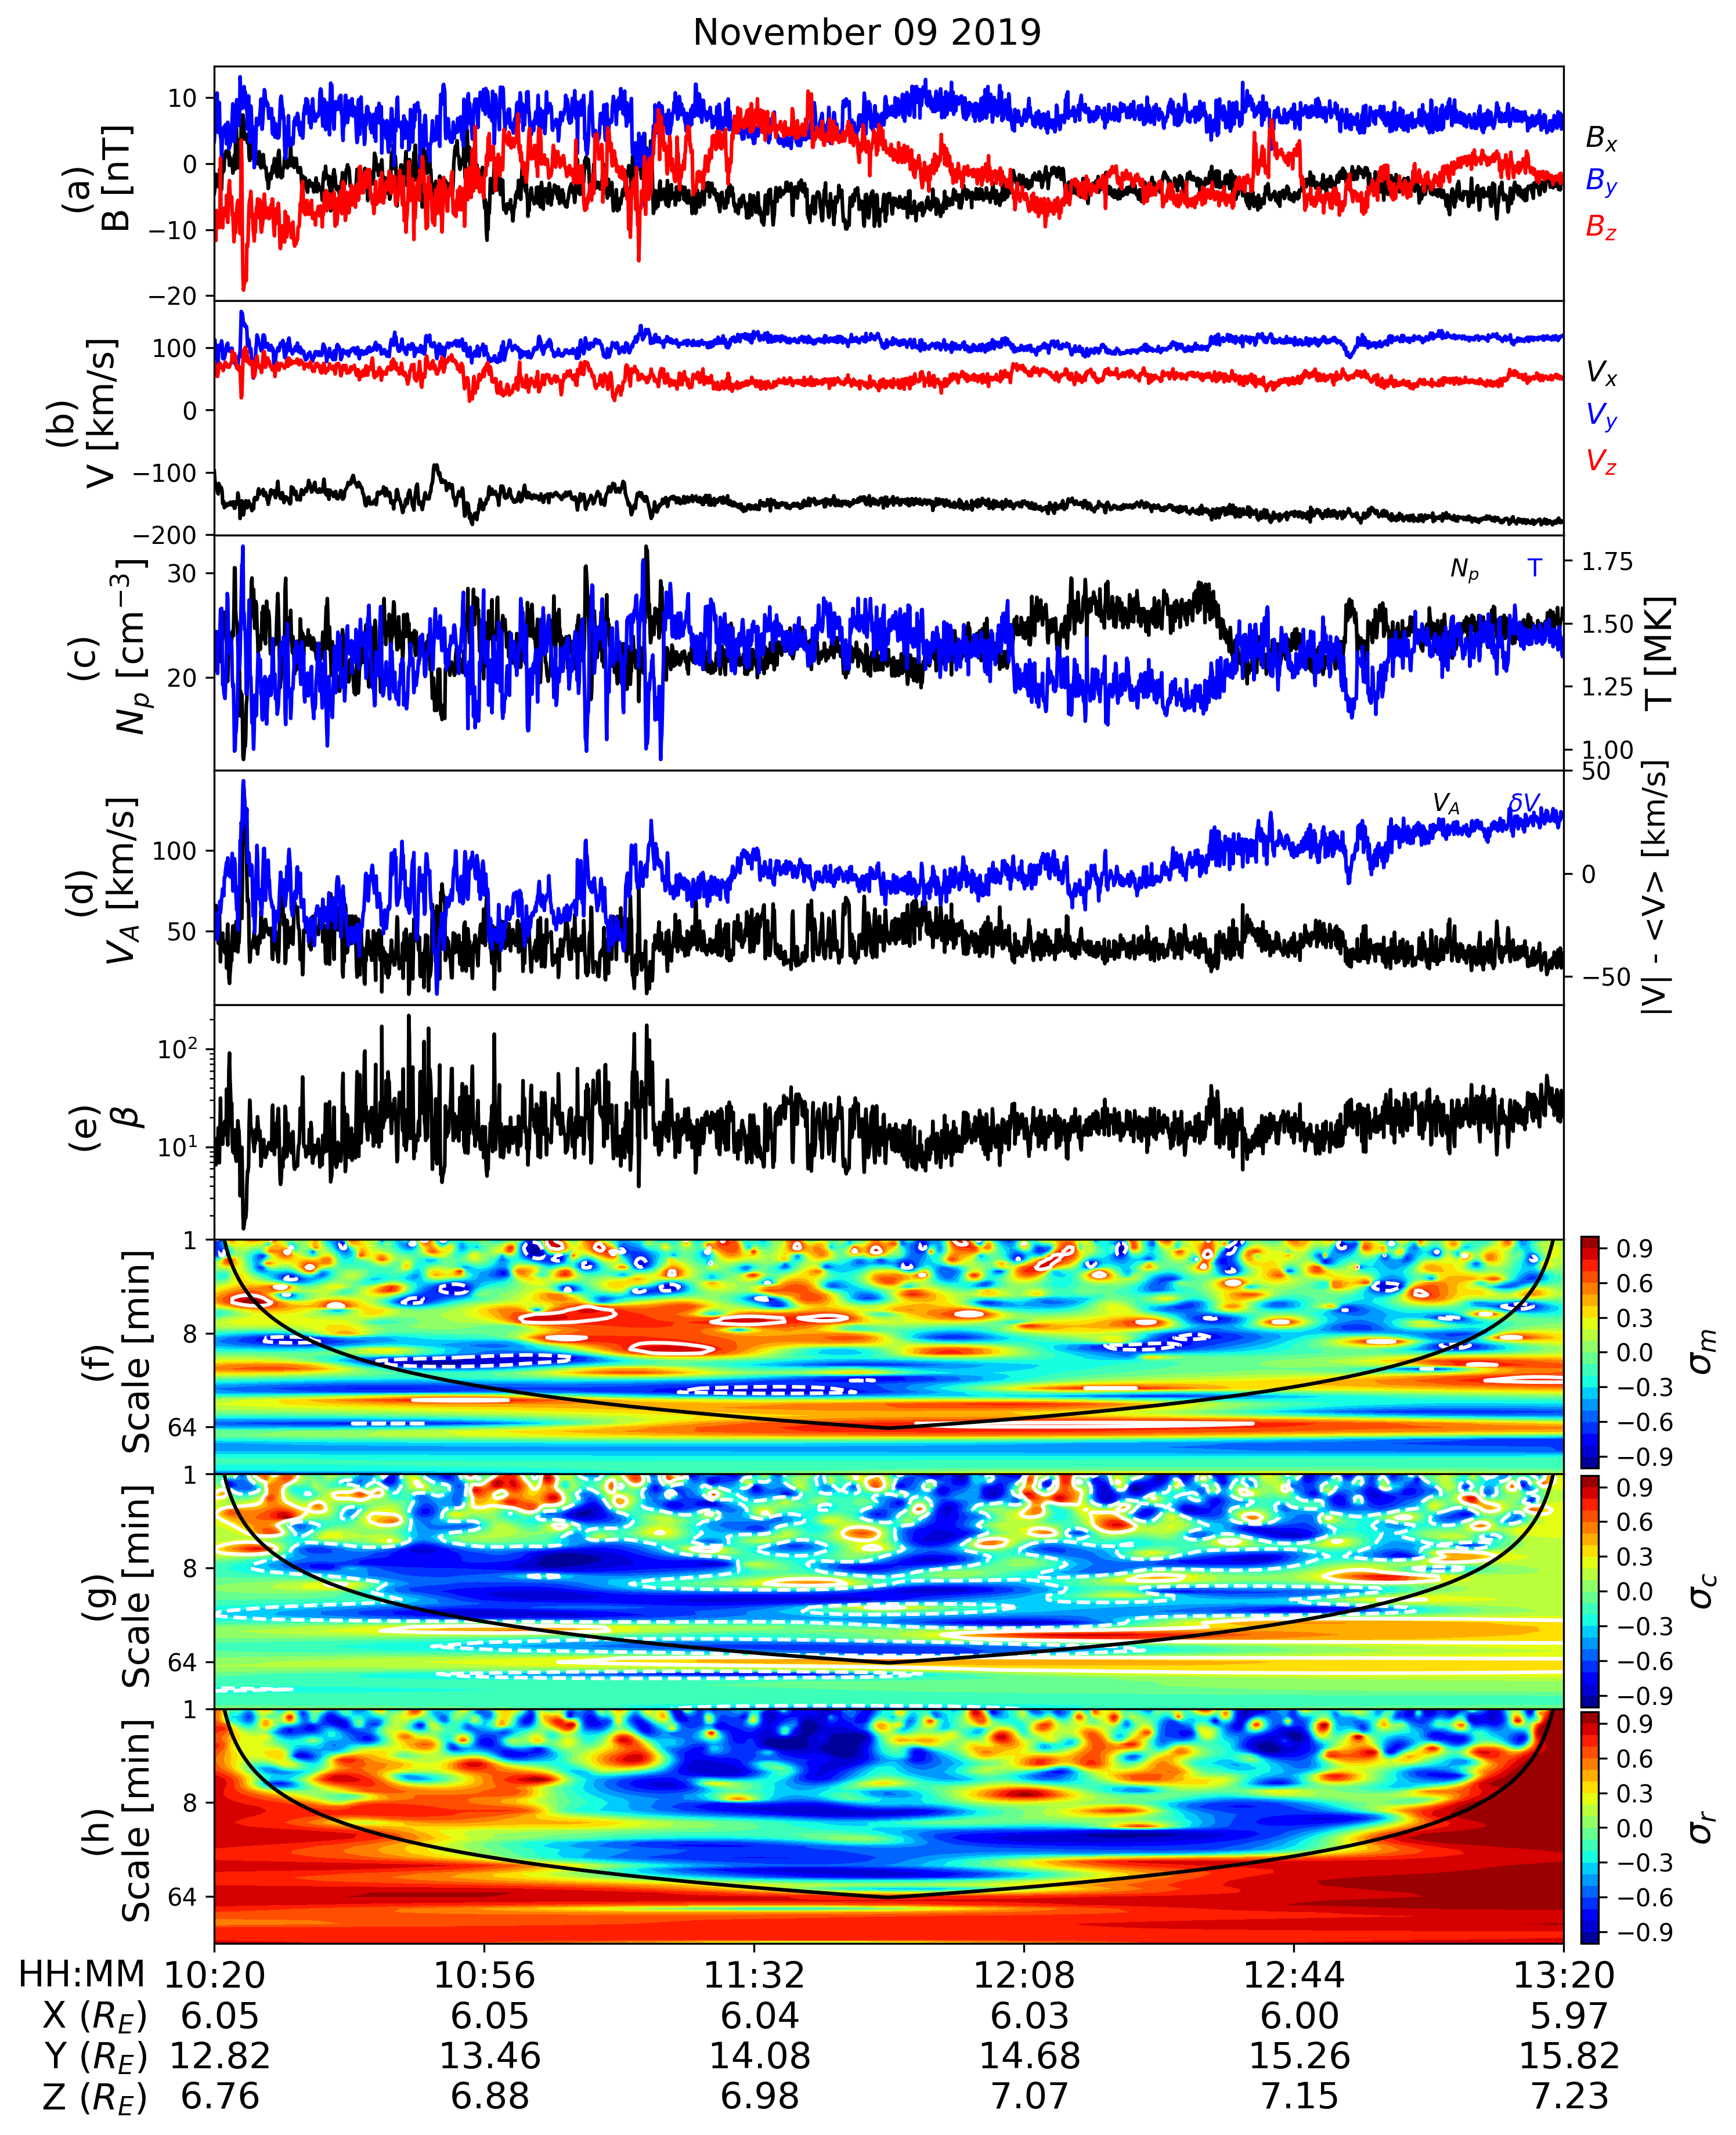
\includegraphics[width=0.8\textwidth]{Figures/Time series/spectrograms_09112019_1020_MMS1.png}
    \caption[Time series data and spectrograms of MHD quantities for 9 November 2019]{Time series of (a) magnetic field, (b) velocity, (c) plasma density and temperature, (d) Alfv\'en speed and velocity fluctuations, (e) plasma beta, and spectrograms of the normalized (f) reduced magnetic helicity, (g) cross helicity, and (h) residual energy found by wavelet analysis, across multiples scales (as indicated by the vertical axes), during a 3 hour period that MMS-1 was in the magnetosheath on 9 November 2019. White contours in panel (f) and (g) represent regions of high reduced magnetic helicity ($|\sigma_m| \geq 0.75$) and regions of low reduced cross helicity ($|\sigma_c| \leq 0.3$), respectively. The black curved line in panels (f)-(h) is the cone of influence.}
    \label{fig:wavelet-spectrograms-mms}
\end{figure}

Structures with local enhanced magnetic helicity are identified with specific criteria: (i) magnetic helicity with absolute values greater than 0.75, (ii) duration between 30 seconds and 3 hours, and (iii) if the event was within the cone of influence, which arises because of finite data segment length \citep{Torrence:1998}. I calculate reduced, normalized forms of magnetic helicity $\sigma_m$, cross helicity $\sigma_c$, and residual energy $\sigma_r$ in 2400-point windows ($\sim$3 hours for MMS and $\sim$2 hours for THEMIS) across the hours-long periods identified in the solar wind and magnetosheath. Figure \ref{fig:spectrograms-interval} displays the spectrograms of reduced magnetic helicity from 10:20-13:30 UT and 11:05-14:05 UT on 9 November 2019. These intervals are calculated from the time series in Figure \ref{fig:wavelet-spectrograms-mms}. Events identified with the wavelet analysis method are marked with a grey interval. The black contours represent event candidates with $|\sigma_m|\geq 0.75$ whereas the white contours indicate events that were established in the final event list. Inside the white contours, a white ``X" marks the absolute local maximum, and the yellow annotations and dashed lines indicate the scale corresponding to a maximum. This scale is taken as the duration of the event, and the time of the peak in reduced $\sigma_c$ is taken to the time-wise midpoint of the event. Therefore, the event interval start time will be the time of the peak in $|\sigma_m|$ minus half of the scale size of the peak. The events identified from this wavelet analysis can be further characterized by implementing the criteria that the events have (iv) corresponding cross helicity with absolute value less than 0.3, to ensure that there is low level of velocity fluctuations and/or (v) negative residual energy, which indicates that the magnetic energy is dominant.
\begin{figure}
    \centering
    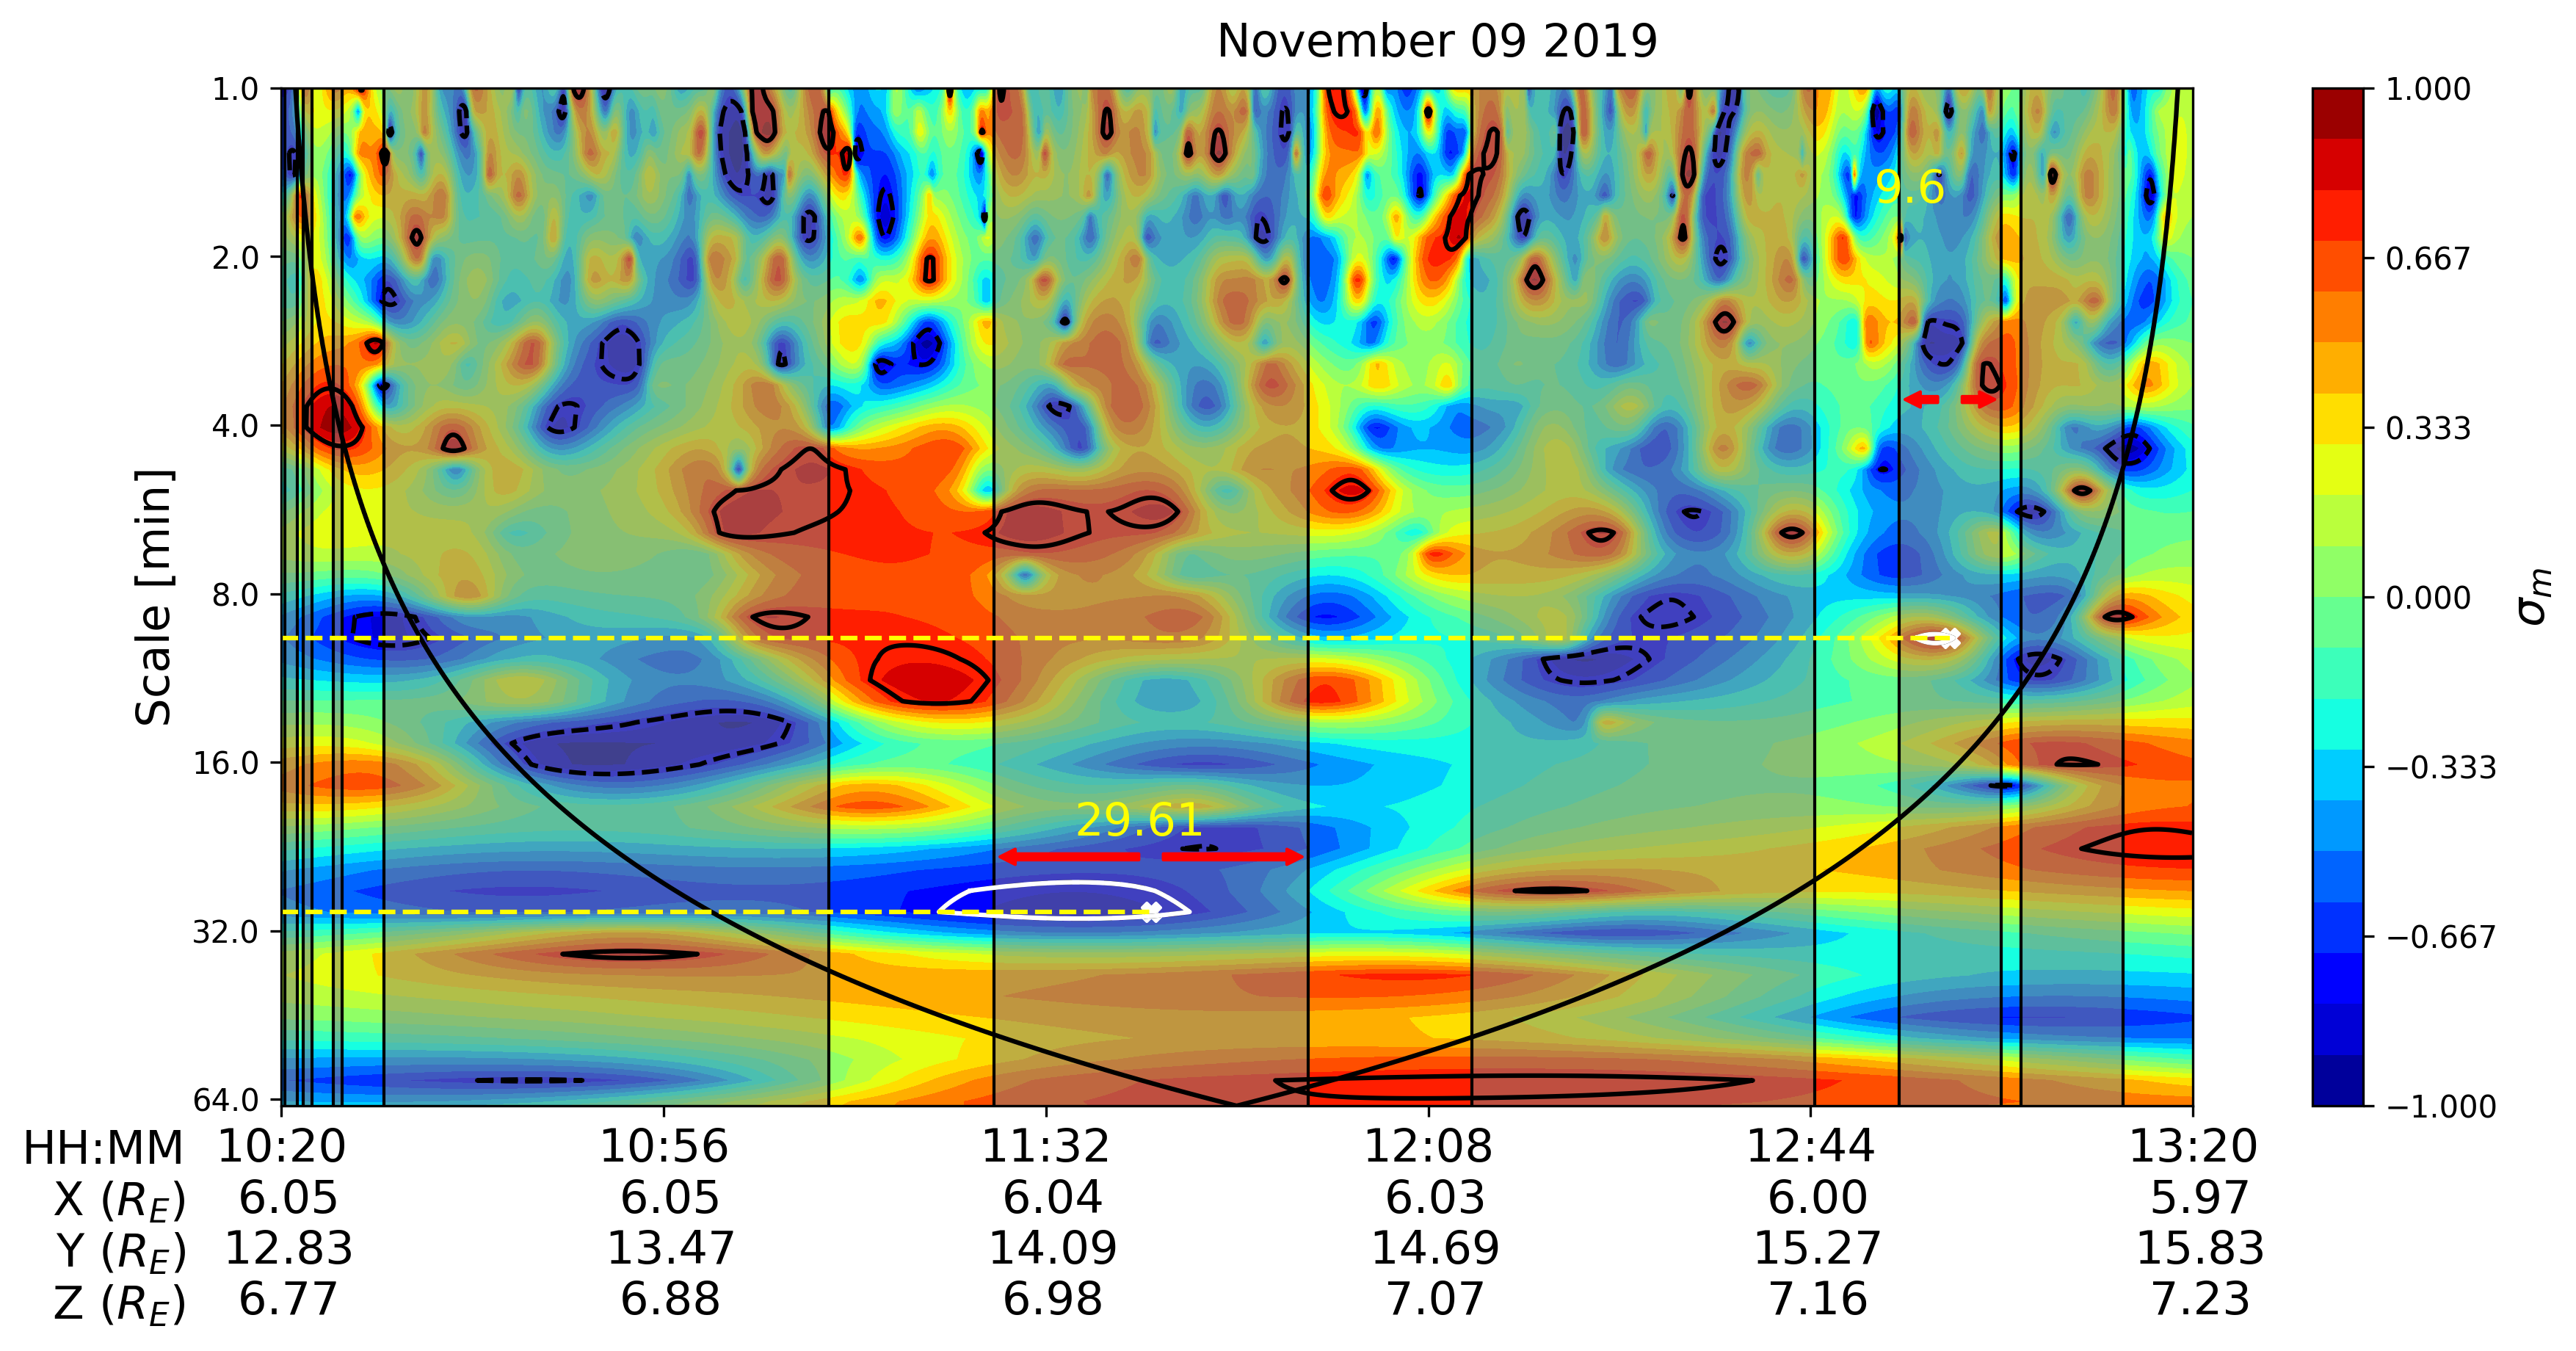
\includegraphics[width=\textwidth]{Figures/Spectrograms/magnetichelicity_wave_events_09112019_1020.png}
    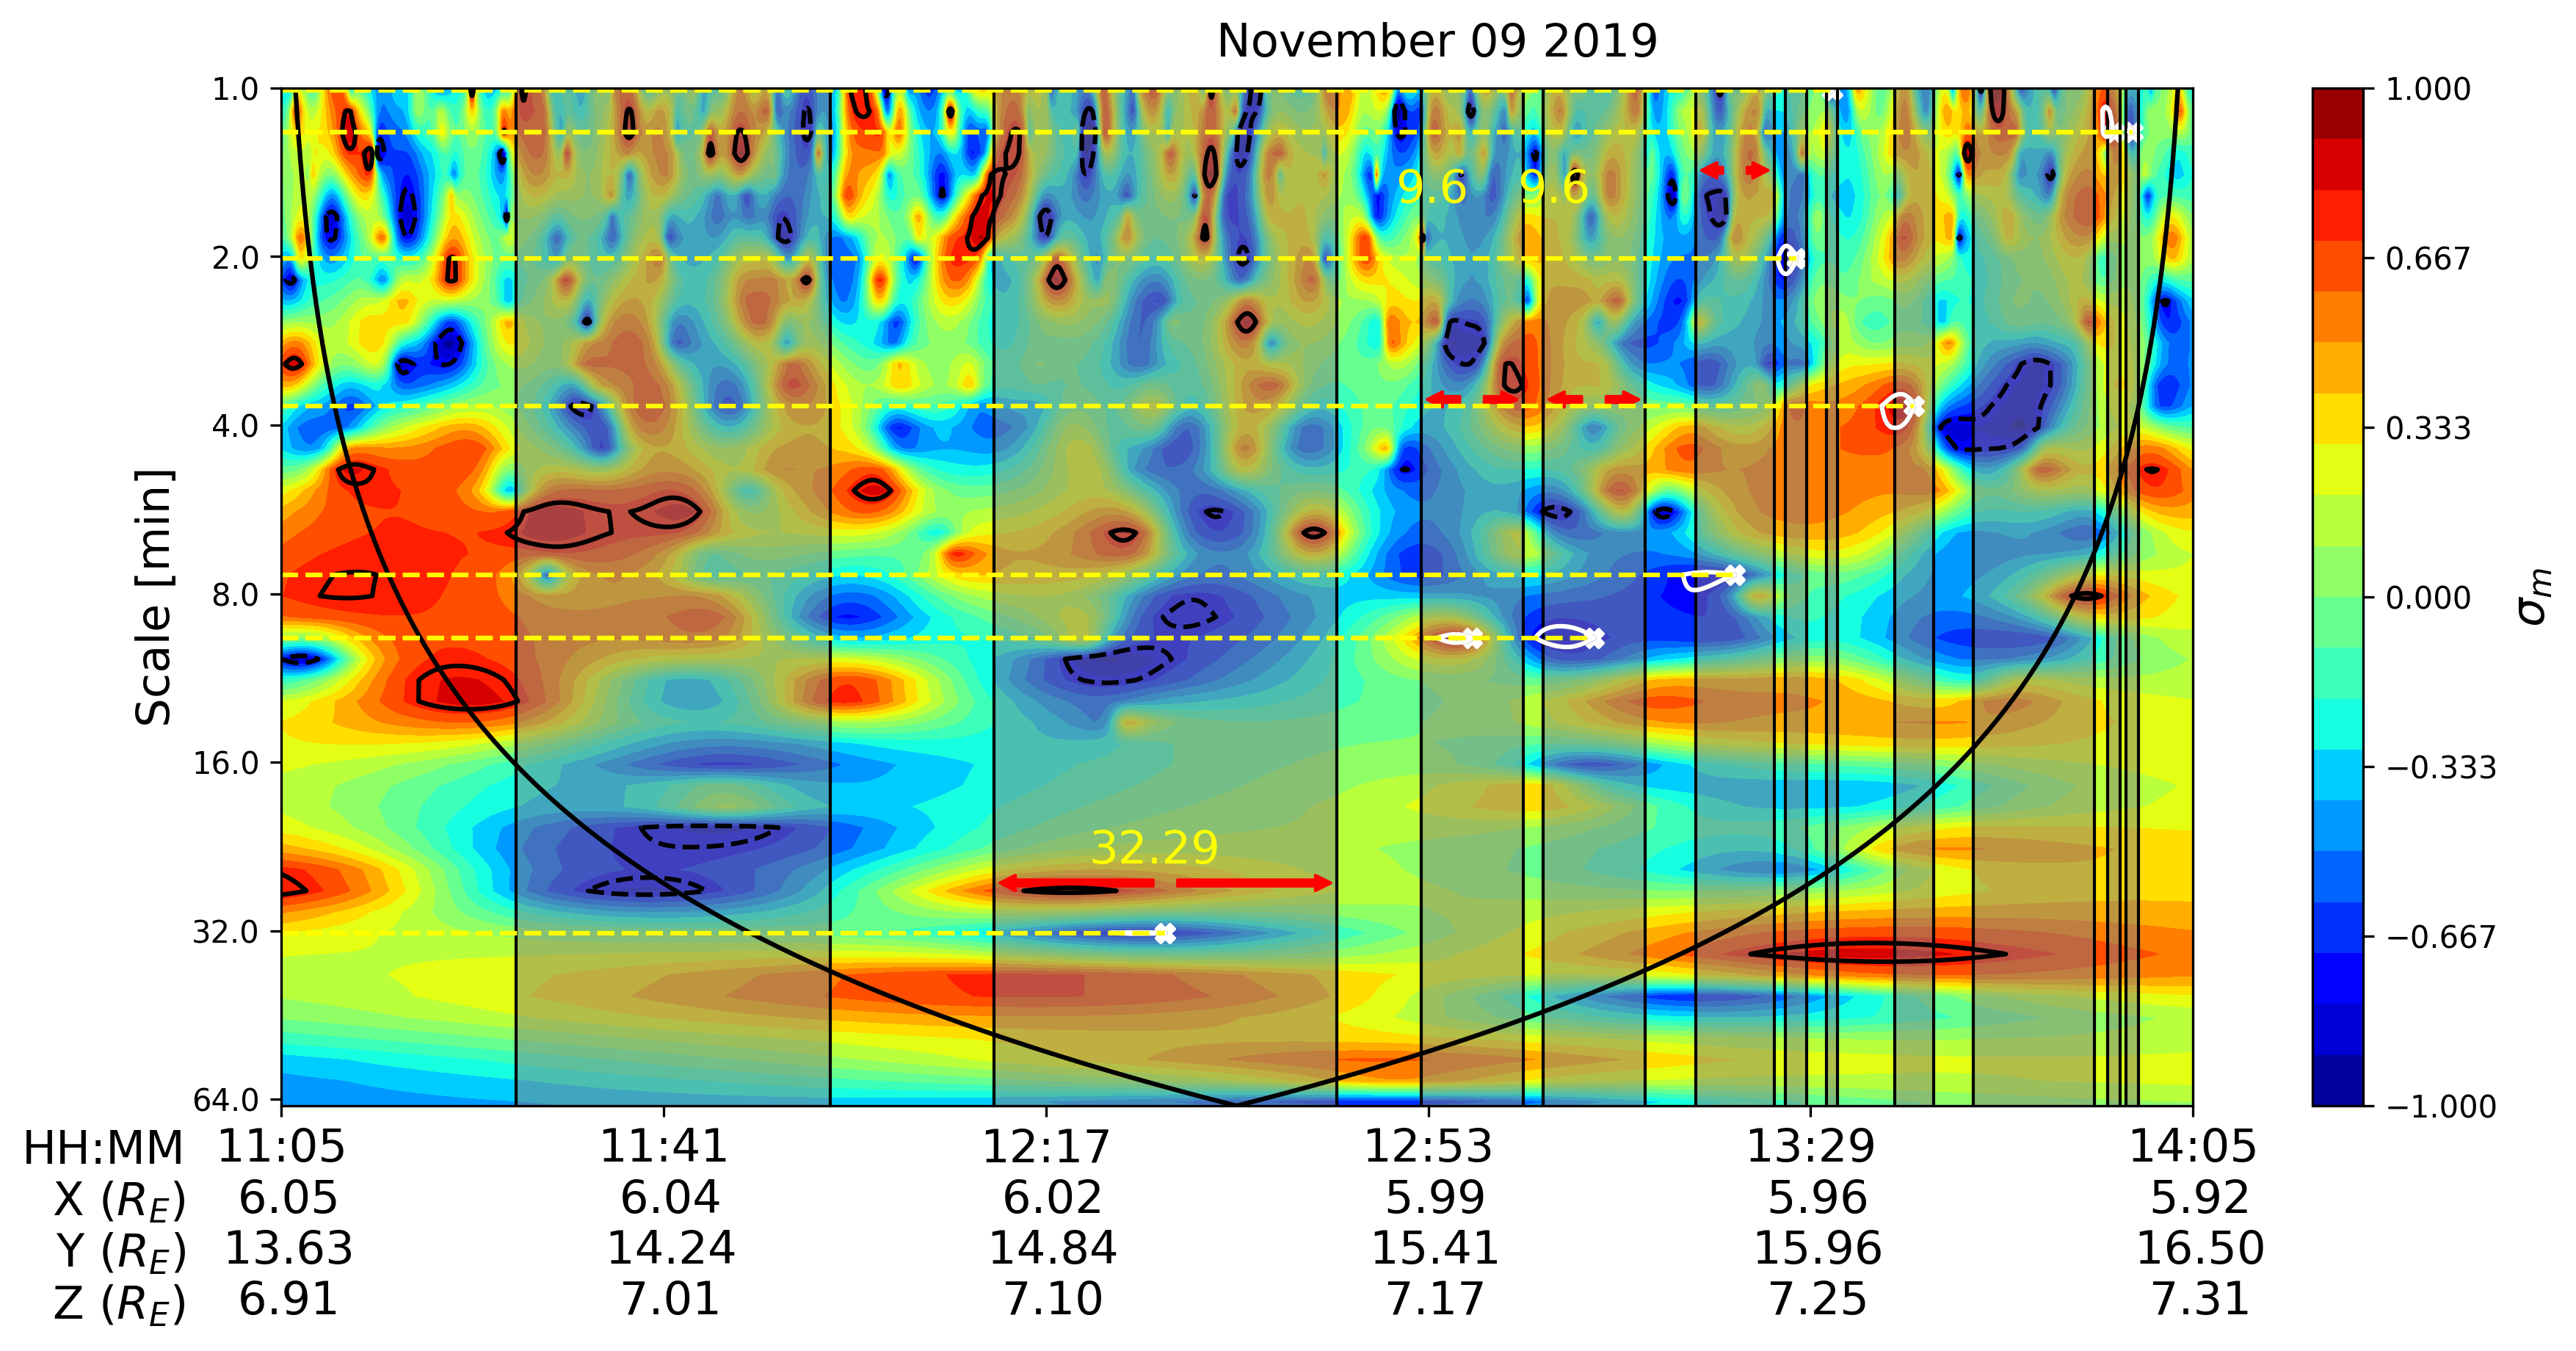
\includegraphics[width=\textwidth]{Figures/Spectrograms/magnetichelicity_wave_events_09112019_1105.png}
    \caption[Diagram of wavelet analysis identification algorithm via spectrograms of MHD quantities]{Spectrograms of reduced magnetic helicity over two overlapping 3-hour period from MMS-1 data on 9 November 2019. Demarcated intervals are identified events via wavelet analysis. Black contours represent regions of high reduced magnetic helicity ($|\sigma_m| \geq 0.75$). White contours represent regions of $|\sigma_m| \geq 0.75$ where the maximum inside the contour is an established event. Yellow dashed lines connect the maximum of the contour to the x-axis (scale) of the maximum. Red arrows indicate half of the scale (duration) on either side of the peak of $\sigma_c$. The black curved line is the cone of influence.}
    \label{fig:spectrograms-interval}
\end{figure}

It can be seen that not all grey event intervals have a white contour and marker for the maximum $\sigma_c$. This is because of the windowed analysis: as the maxima in reduced magnetic helicity are recorded in each window, there will be overlapping events identified. The intervals in Figure \ref{fig:spectrograms-interval} are overlapping by 600 data points (45 minutes for MMS data). After all the windows are searched, the compiled event list is then processed to eliminate overlapping events. By comparing two adjacently overlapping events and keeping the one with the highest maximum $|\sigma_m|$, this is repeated until there are no overlapping events left.


\section{Event categorization}\label{sec:wavelet-results}
There were 4260 events identified from the wavelet analysis in the magnetosheath across 1051 hours. For the solar wind, there were 3193 events identified across 676 hours via wavelet analysis. The occurrence rate for events in the solar wind from the wavelet method is about 4.7 events/hour and for the magnetosheath the corresponding rate is about 4.0 events/hour. Table  \ref{tab:regions-wavelet-summary} summarizes the events identified with the wavelet analysis algorithm.
\begin{table}
    \centering
    \caption{Summary table for identified events in the solar wind and magnetosheath via wavelet analysis as described in Section \ref{sec:wavelet-algorithm}.}
    % \begin{tabular}{rcccccc}
% \hline
%  & Hours  & Events &  Avg. duration &  Avg.    &  Avg. scale & Event rate \\
%  &           &           & [mins]   &  B [nT]      &  size [km]  & [\#/hour] \\
% \hline
% \textit{Solar wind}     & 676   &  3193  & 7.40 & 4.93  & 161241.93 & 4.723 \\
% \textit{Magnetosheath}  & 1051  &  4260  & 8.76 & 20.21 & 110801.05 & 4.053 \\
% \hline
% \end{tabular}

\begin{tabular}{rccc}
\hline
                        & Observation   & Events &  Event rate \\
                        & period [hrs]  &        &  [\#/hour]  \\
\hline
\textit{Solar wind}     & 676           &  3193  & 4.723 \\
\textit{Magnetosheath}  & 1051          &  4260  & 4.053 \\
\hline
\end{tabular}
    \label{tab:regions-wavelet-summary}
\end{table}

Properties of the magnetic structures are recorded during the identification process. Table \ref{tab:wavelet-stats} summarizes the statistical values for the identified events. The average duration of the events is 7.40 and 8.76 minutes for the solar wind and magnetosheath, respectively. In the solar wind, there are a large number of events with an average magnetic field of less than 10 nT, whereas in the magnetosheath there are relatively much fewer events with $\langle B\rangle < 10$ nT. The median magnetic field magnitude in the solar wind is 4.6 nT for events identified with wavelet analysis, and in the magnetosheath this number is 16.5 nT. As shown in Table \ref{tab:wavelet-stats}, the duration of the events has similar ranges for the two regions. However, for the scale sizes of the events in the magnetosheath, they range from $\sim$1507 km to 1.287$\times 10^6$ km, with a median and mean of 34410 km, $\sim$5.4 $R_E$ and 1.108$\times 10^5$ km, $\sim$17.4 $R_E$, respectively. In the solar wind, the corresponding values are from 8975.2 km to 2.107$\times 10^6$ km, and a median (mean) of 54440 (1.612$\times 10^5$) km, $\sim$8.5 (25.3) $R_E$. It is important to note that the calculations of scale size cannot be considered as physically reliable as the calculations from the GS-based method since the specificity of the wavelet analysis identification method relies on factors such as data segment length and choice of wavelet basis, in addition to the calculations being done in the spacecraft frame of reference.
\begin{table}
    \centering
    \caption[Statistical values for the physical quantities of structures identified with wavelet analysis]{Statistical values for the physical quantities of the structures identified in the magnetosheath (top) and solar wind (bottom) with wavelet analysis.}
    \begin{tabular}{lccccc}
\hline
       & Minimum & Maximum & Mean & Median & Std. Dev. \\
\hline
Duration [min]         & 0.517    & 59.221             & 8.761              & 2.617     & 12.6 \\
Velocity [km/s]        & 13.653   & 567.539            & 220.381            & 214.361   & 75.4 \\
Temperature [10$^6$ K] & 0.601    & 31.611             & 2.908              & 2.200     & 2.3  \\
$<B>$ [nT]             & 2.344    & 85.790             & 20.213             & 16.473    & 12.2 \\
Scale size [km]        & 1506.944 & 1.287$\times 10^6$ & 1.108$\times 10^5$ & 3.441$\times 10^4$ & 1.6$\times 10^5$ \\

\hline \hline

Duration [min]         & 0.560    & 59.221             & 7.402              & 2.400     & 10.6 \\
Velocity [km/s]        & 235.264  & 664.001            & 367.580            & 342.591   & 87.4 \\
Temperature [10$^6$ K] & 0.114    & 16.946             & 2.600              & 0.685     & 3.4 \\
$<B>$ [nT]             & 0.543    & 29.372             & 4.935              & 4.576     & 2.5 \\
Scale size [km]        & 8975.252 & 2.107$\times 10^6$ & 1.612$\times 10^5$ & 5.444$\times 10^4$ & 2.4$\times 10^5$ \\

\hline
\end{tabular}

    \label{tab:wavelet-stats}
\end{table}

Table \ref{tab:wavelet-event-summary} categorizes the events identified via wavelet analysis based on meeting certain MHD criteria. Over half of the events in the solar wind have characteristics of static flux ropes ($|\sigma_m|\geq 0.75$, $|\sigma_c|\leq 0.3$, $\sigma_r<0$), whereas in the magnetosheath there are fewer events (approximately one-third) that meet these criteria.
\begin{table}
    \centering
    \caption{Summary table of events meeting certain MHD criteria for events identified via wavelet analysis in the magnetosheath and solar wind.}
    \label{tab:wavelet-event-summary}
    \begin{tabular}{rcc}
\hline
{} & Solar wind & Magnetosheath \\
\hline
$|\sigma_m|\geq 0.75$                        & 3193 & 4260  \\
$|\sigma_m|\geq 0.75$, $|\sigma_c|\leq 0.3$  & 1821 & 2490  \\
$|\sigma_m|\geq 0.75$, $\sigma_r<0$          & 2156 & 2468  \\
$|\sigma_m|\geq 0.75$, $|\sigma_c|\leq 0.3$, $\sigma_r<0$ & 1144 & 1567 \\
\hline
%\multicolumn{3}{c}{$^c$in the magnetosheath and solar wind.}
\end{tabular}
\label{tab:wavelet-event-summary}

% sw_eventCount + msh_eventCount
\end{table}
The distribution of the reduced cross helicity and residual energy for all identified events in the solar wind and magnetosheath is shown in Figure \ref{fig:mhd_histogram-wavelet}. The histogram shows the averaged, reduced MHD quantities of the events identified by the wavelet method. Figure \ref{fig:mhd_histogram-wavelet} shows flatter distributions of reduced cross helicity $\sigma_c$ in the magnetosheath than in the solar wind. The reduced cross helicity distribution maintains a peak around $\sigma_c=0$ in both regions in Figure \ref{fig:mhd_histogram-wavelet}, with the solar wind having a steeper shape. The reduced residual energy has a peak at $\sigma_r=-1$, with values that are nearly evenly distributed between $(-1,1)$.

\begin{figure}
    \centering
    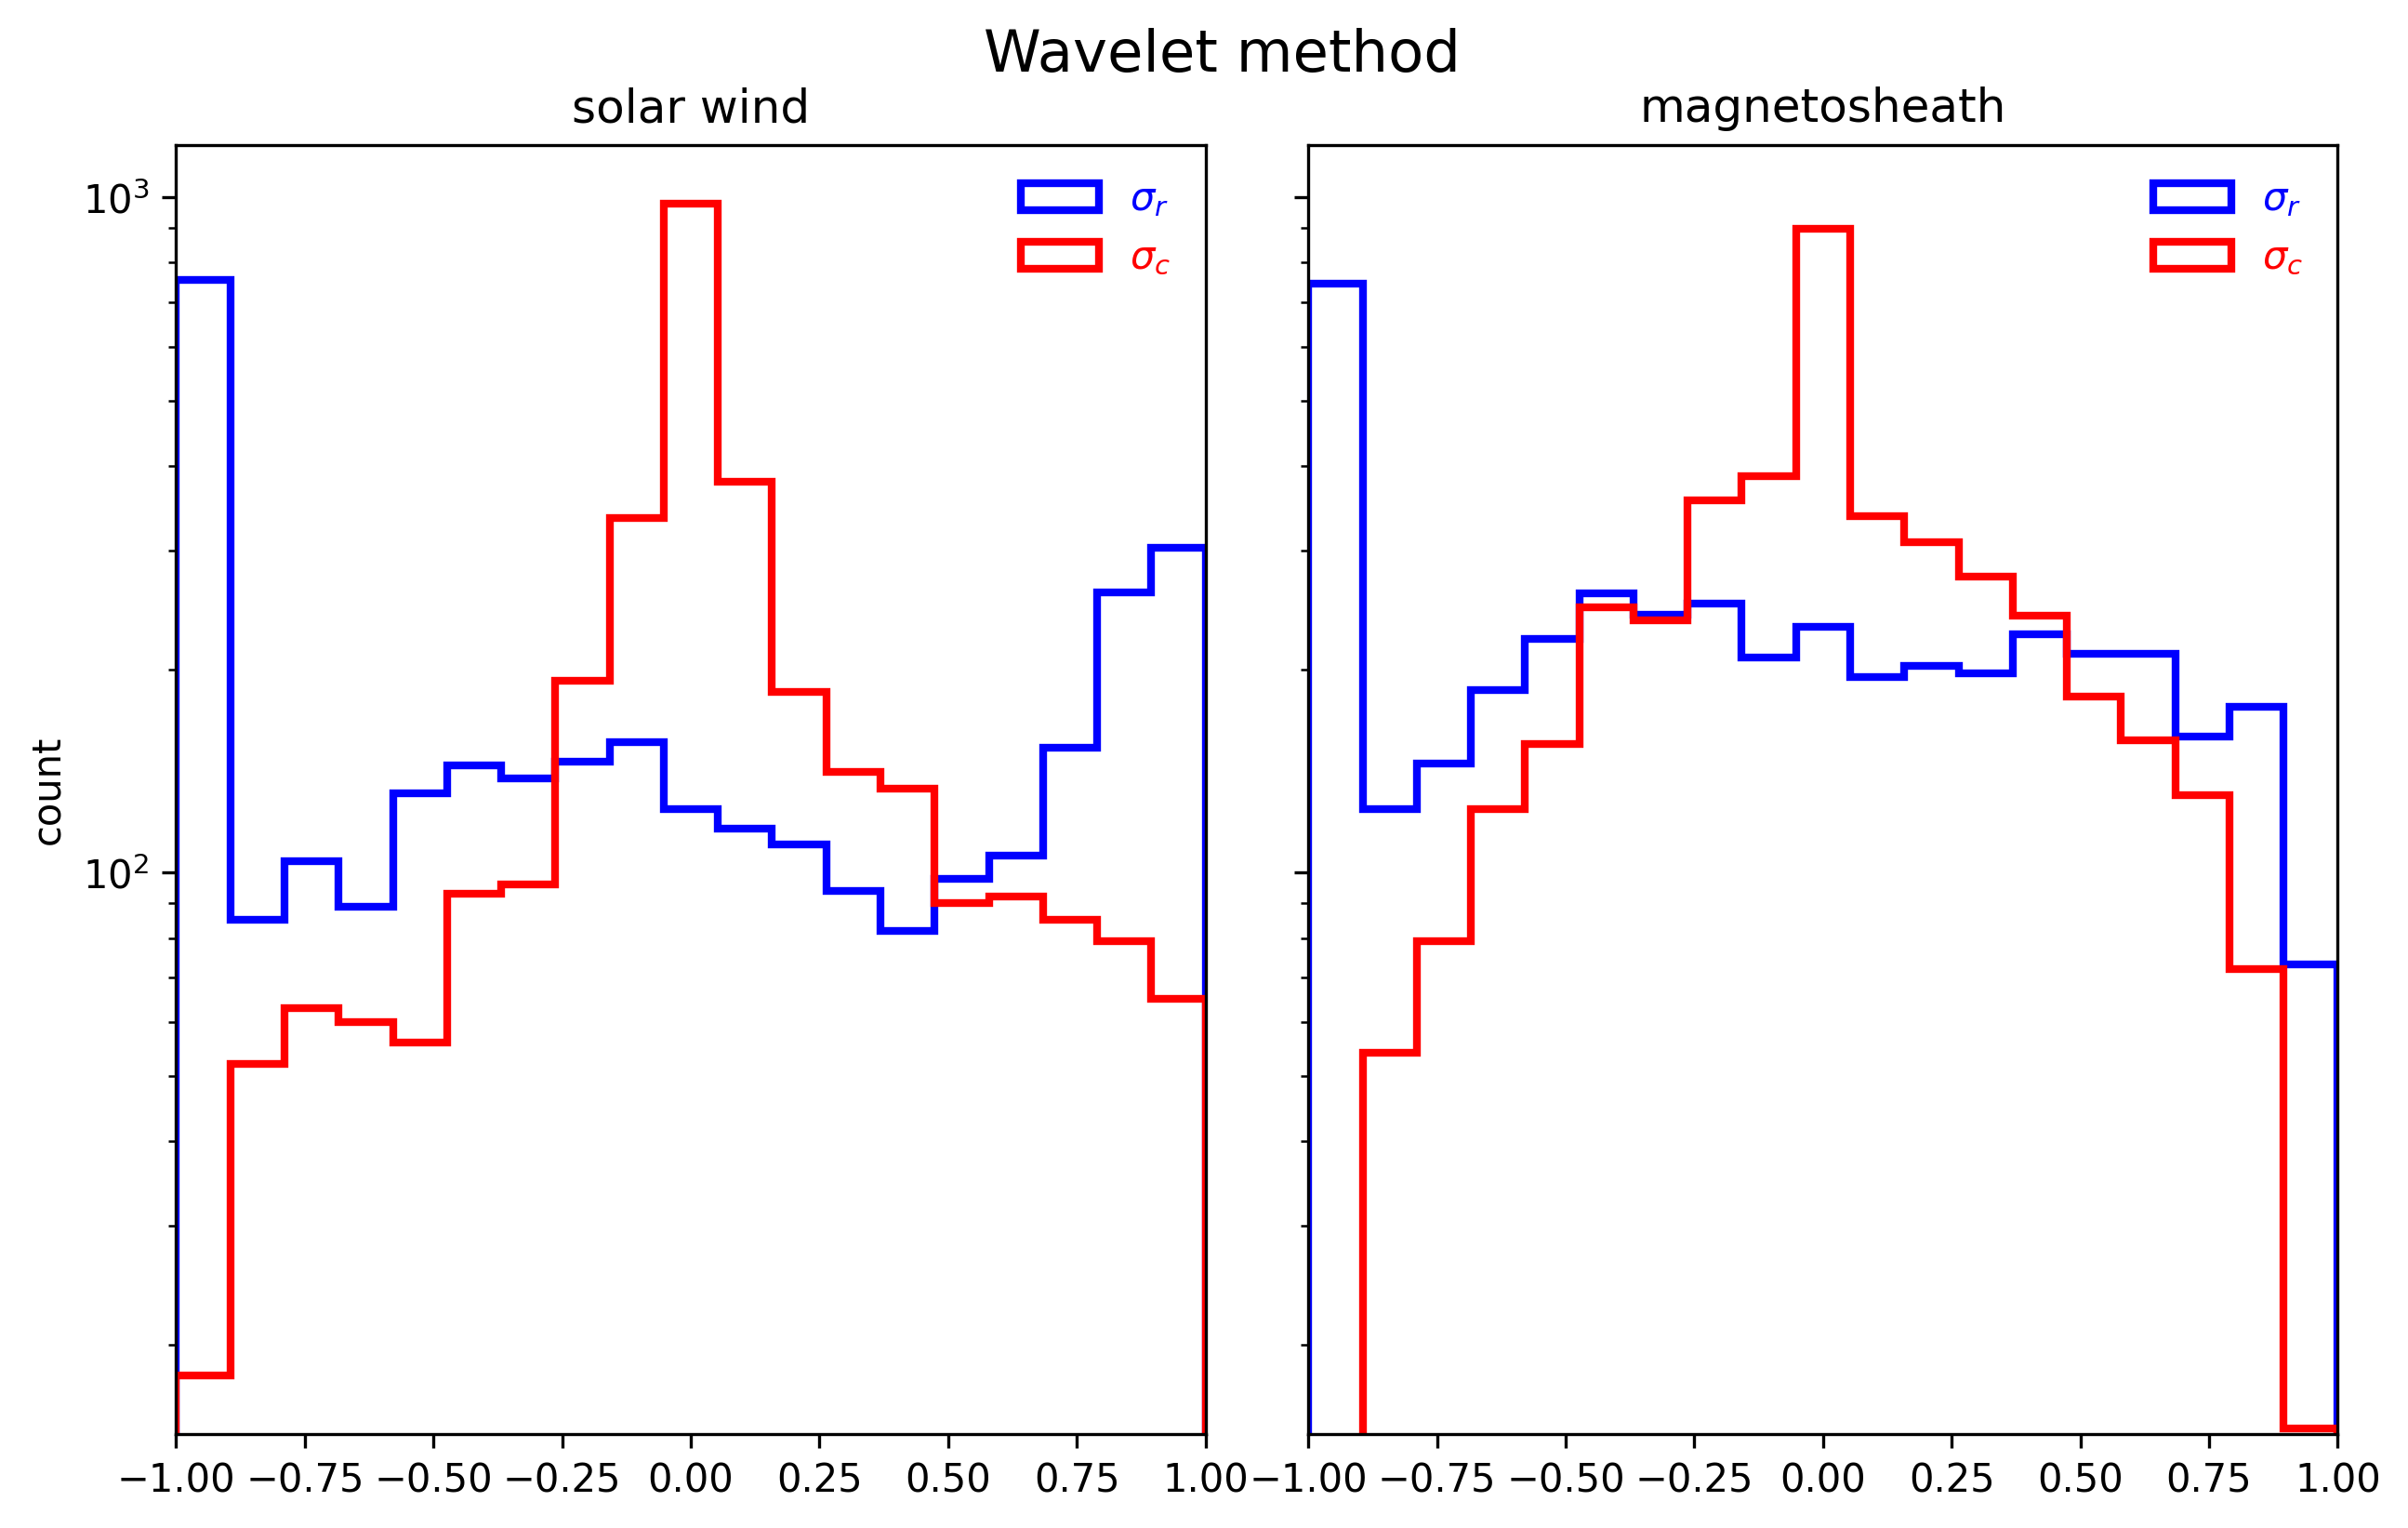
\includegraphics[width=\textwidth]{Figures/Histograms/sigr_sigc_wavelet.png}
    \caption[Reduced cross helicity and reduced residual energy for all events identified via wavelet analysis]{Histograms of reduced cross helicity $\sigma_c$ (red) and reduced residual energy $\sigma_r$ (blue) for all solar wind (left) and magnetosheath events (right) identified via the wavelet method.}
    \label{fig:mhd_histogram-wavelet}
\end{figure}
\chapter{Chapter 4. Grad-Shafranov reconstruction and automated identification algorithm} \label{ch:ch4} % of magnetic structures

\section{The Grad-Shafranov equation}
%\input{Chapters/Introduction/GS_equation}
The Grad-Shafranov (GS) equation describes the force balance between the Lorentz force and the gradient of the thermal pressure \citep{Sonnerup:1996, Hau:1999}, as given below,
\eql{eq:GS}{\delsq A = \npdv{2}{A}{x} + \npdv{2}{A}{y} = -\mu_0 \dv{P_t}{A} = - \mu_0\dv{}{A}\p{p + \frac{B_z^2}{2\mu_0}}.}

\subsection{Derivation of the original GS equation}
Starting with the magnetic field as a function of the magnetic vector potential and balancing the gradient of the pressure with the Lorentz force,
\eql{eq:B}{\Bvec = \delcross\Avec = \del\Avec\cross\zhat + B_z\zhat}
\eql{eq:gradp}{\grad p = \jvec\cross\Bvec = j_z\zhat\cross\Bvec_\perp + \jvec_\perp\cross B_z\zhat}

\noindent Using Ampere's law to determine the components of the current density $\jvec$,
\eql{eq:Amperes}{\begin{split}
    \delcross\Bvec &= \mu_0\jvec \\
    \delcross\p{\delcross\Avec} & = \mu_0\jvec \\
    \delcross\pp{\grad\Avec\cross\zhat + B_z\zhat} &= \mu_0\pp{j_z\zhat + \jvec_\perp} \\
\end{split}}
The $\zhat$ and perpendicular components of the current density are then found by,
\eql{eq:jz}{\begin{split}
    \mu_0 j_z\zhat &= \delcross\p{\grad\Avec\cross\zhat} \\
    &= \p{\deldot\zhat}\grad\Avec - \p{\deldot\del\Avec}\zhat \\
   j_z\zhat &= -\frac{1}{\mu_0}\delsq\Avec\zhat \\
\end{split}}
\eql{eq:jperp}{\begin{split}
    \mu_0\jvec_\perp &= \delcross B_z\zhat \\
    \jvec_\perp &= \frac{1}{\mu_0}\grad B_z\cross\zhat \\
\end{split}}

\noindent Simplifying the $\zhat$ and perpendicular terms of the pressure gradient (\ref{eq:gradp}),
\eql{eq:jzBperp}{\begin{split}
    j_z\zhat \cross\Bvec_\perp &= -\frac{1}{\mu_0}\delsq\Avec\zhat\cross\p{\grad\Avec\cross\zhat} \\
    &= -\frac{1}{\mu_0}\pp{\p{\delsq\Avec\zhat\cdot\zhat}\del\Avec - \p{\delsq\Avec\zhat\cdot\grad\Avec}\zhat} \\
    &= -\frac{1}{\mu_0}\p{\delsq\Avec} \grad\Avec \\
\end{split}}
\eql{eq:jperpBz}{\begin{split}
    \jvec_\perp\cross B_z\zhat &= \p{\frac{1}{\mu_0}\grad B_z\cross\zhat}\cross B_z\zhat \\
    &= \frac{1}{\mu_0}\pp{\p{\zhat\cdot\del}B_z\zhat - \p{B_z\zhat\cdot B_z\zhat}\del} \\
    &= -\frac{1}{\mu_0}B_z\grad B_z
\end{split}}

\noindent and substituting them into the respective right hand side of (\ref{eq:gradp}), we arrive at the form for the Grad-Shafranov equation (\ref{eq:GS}):
\eq{\begin{split}
    \grad p &= -\frac{1}{\mu_0}\p{\delsq\Avec}\grad\Avec - \frac{1}{\mu_0}B_z\grad B_z \\
    \p{\delsq\Avec}\grad\Avec &= -\mu_0\p{\grad p+ \frac{1}{\mu_0}B_z\grad B_z} \\
    \p{\delsq\Avec}\grad\Avec &= -\mu_0 \p{\dv{p}{A}\grad\Avec + \frac{1}{\mu_0}B_z\dv{B_z}{A}\grad\Avec} \\
    \delsq\Avec &= -\mu_0\p{\dv{p}{A} + \frac{1}{\mu_0}\dv{B_z}{A}} \\
\end{split}}

\eql{eq:gradp2}{\delsq\Avec = -\mu_0\dv{}{A}\p{p + \frac{B_z^2}{2\mu_0}}}

\subsection{Derivation of the extended GS equation}
The implementation by \cite{Chen:2021} utilizes the extended GS method, which still seeks to find the double-folding pattern between two $P_t'$ versus $A'$ curves, but with $A'=(1-\alpha)A$ and $P_t'=\p{1-\alpha}p + \p{1-\alpha}^2\frac{B_z^2}{2\mu_0} + \alpha\p{1-\alpha}\frac{B^2}{2\mu_0}$.  The factor $\alpha$ is a proportionality constant, which for a field-aligned flow is the average Alfv\'en Mach number squared, $\alpha=\langle M_A\rangle^2 \approx const$ in a frame of reference moving with the structure governed by the GS equation. The extended GS equation \citep{Teh:2018, Sonnerup:2006} is:
\begin{equation}
    \nabla^2 A' = -\mu_0\frac{\mathrm{d}}{\mathrm{d}A'}\left[\left(1-\alpha\right)p + \left(1-\alpha\right)^2\frac{B_z^2}{2\mu_0} + \alpha\left(1-\alpha\right)\frac{B^2}{2\mu_0} \right]
    \label{eq:GSextended}
\end{equation}
which simplifies to the original GS equation (\ref{eq:GS}) when $\alpha\equiv 0$. The extended GS method allows us to identify structures with significant remaining plasma flow aligned with the local magnetic field in a proper frame of reference \citep{Chen:2022}.

\section{Automated GS-based detection of SFRs}
In both the original and the GS-type equations, the transverse pressure $P_t$, and its equivalent $P_t'$, are single variable functions of the magnetic flux function $A$ ($A'$ for the GS-type with $\alpha\equiv const$). With this feature, one can recover the 2D cross-section of a flux rope structure from the 1D spacecraft data by solving the initial value problem based on the GS equation, i.e., by carrying out the GS reconstruction procedures \citep{Hau:1999, HuSonnerup:2002, Hu:2017}. The GS-based techniques in this study consist of the GS-type reconstruction and the extended GS-based automated detection. Considering the complicated environment from the solar wind to the magnetosheath, we adopt the GS-type reconstruction in this study for selected events only.

A cross section of a cylindrical flux rope structure is fully characterized by the 2D scalar flux function $A(x, y)$, and the field-line invariants $\p{B_z,J_z,p, P_t}$ vary among the nested cylindrical flux surfaces while remaining constant on each distinct surface with a distinct $A$ value \citep{Hu:2018}. As a spacecraft passes through the cross section of a magnetic flux rope with closed transverse field lines, it crosses the same set of magnetic field lines twice, the second time being in reverse order as the first half of the crossing. Therefore, the measured magnetic flux function $A$ associated with the field lines traversed by the spacecraft is double-folded, meaning there is a turning point at which an extremum in $A$ is reached. These features, especially the double-folding pattern, are the basis for the GS reconstruction-based identification algorithm \citep{Hu:2018}. Figure \ref{fig:GSreconstruction_Hu2017} shows diagram of a reconstruction of a magnetic cloud event and the associated flux rope structure. The cross section from the reconstruction algorithm can be seen as well as its relation to the magnetic field lines of the flux rope structure. A more detailed description of the implementation \citep{Hu:2018}, including a flowchart of the flux rope detection algorithm, can be found in Appendix \ref{ch:gs-flowchart}, and online\footnote{\url{fluxrope.info/flowchart.html}}.

\begin{figure}
    \centering
    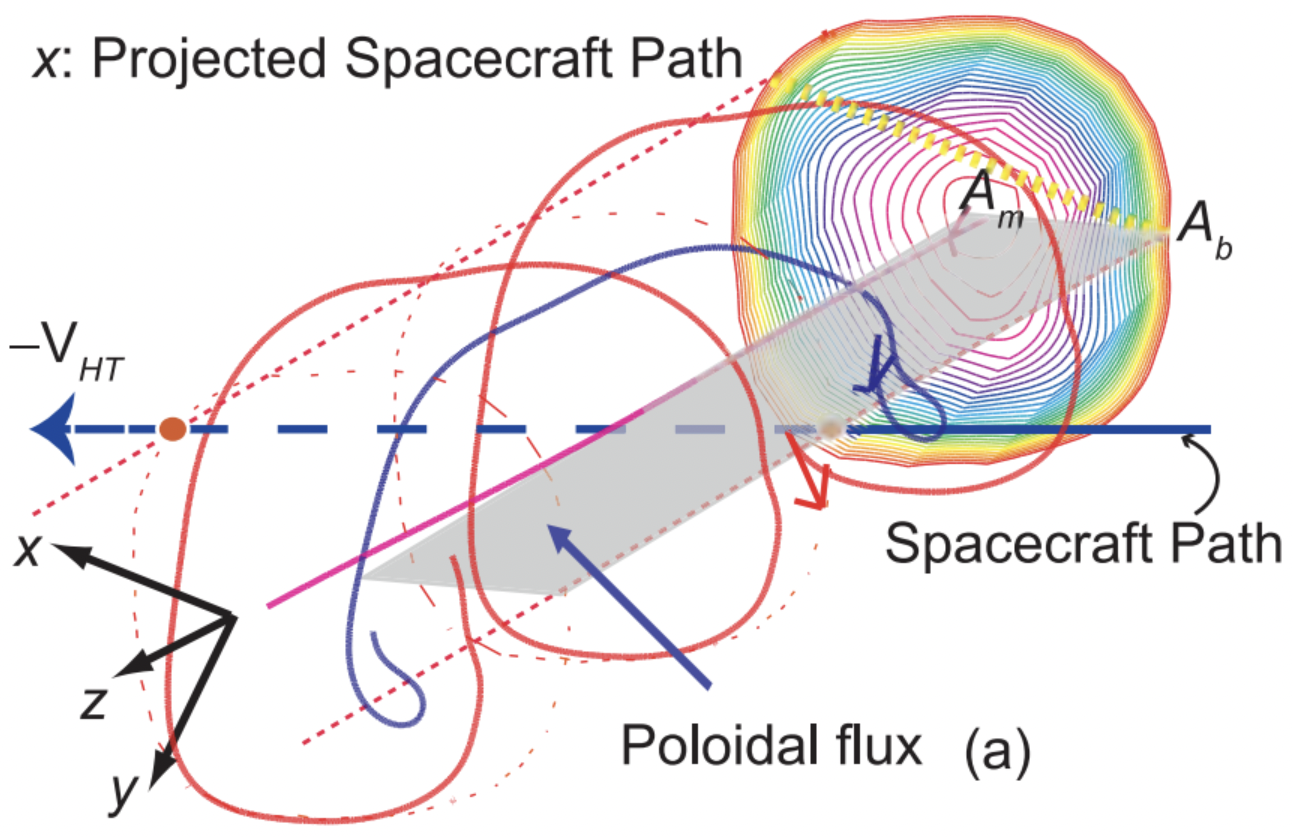
\includegraphics[width=0.75\textwidth]{Figures/Hu2017_5a.png}
    \caption[2D cross section view of a flux rope structure reconstruction] {View of a flux rope structure reconstruction for a magnetic cloud event \citep{Hu:2015} as a spacecraft passes through it. The 2D cross section and selected associated magnetic field lines (red and blue twisted lines) along the flux rope axis ($z$-axis). $A_m$ and $A_b$ mark the magnetic flux function $A$ at the center and boundary, respectively, of the reconstruction. The poloidal flux can also be obtained through the reconstruction algorithm.} %$\Phi_p = |A_m-A_b|\cdot L_{eff}$ along the effective length of the $z$-axis (shaded portion)
    \label{fig:GSreconstruction_Hu2017}
\end{figure}

% Determination of the cylindrical z-axes
The GS-based algorithm starts by moving a window continually through an entire data segment with variable window sizes in turn, ranging from the minimum duration of approximately 10 data points with cadence $\Delta t$, i.e. 10$\Delta t$, to the maximum duration of 343 data points to cover a wide range of SFR duration, while taking into account limited computing resources. The maximum duration corresponds to approximately 17 minutes for the THEMIS data, and 25 minutes for the MMS data. The \textit{in situ} magnetic field and plasma data from a specified window of time are first transformed into the co-moving frame, notably the de Hoffmann-Teller frame \citep{deHoffman-Teller:1950}. Through a trial-and-error process, the optimal orientation of the $z$-axis is determined. A trial $z$-axis is represented by the azimuthal and polar angles, $\phi$ and $\theta$, in the GSE coordinate system. The azimuthal angle $\phi$ is the longitude of the SFR $z$-axis, which measures the angle between the GSE $X$-direction and the projection of the $z$-axis onto the $XY$-plane. The polar angle $\theta$ is the angle between the SFR $z$-axis and the $Z$-direction. To do so, we select trial values for $\phi$ and $\theta$, and calculate the transverse pressure $P_t'$ along the spacecraft path, as shown in Equation (\ref{eq:GSextended}). The plot of $P_t'$ versus $A'$ may have a turning point where $P_t'$ along the spacecraft path splits into two parts, with an extreme $A'$ value near this turning point, typically for an SFR structure. This is where the magnetic field $B_y$ component changes sign because of the field line geometry of a helical structure. Figure \ref{fig:Pt-vs-A} represents such a $P_t'$ versus $A'$ plot, with two distinct portions joining near a turning point with a minimum $A'$ value. We evaluate the quality of the folding (or overlapping) of the two parts of $P_t'$ versus $A'$ by two metrics, $R_{diff}$ (the point-wise difference residue between the two parts) and $R_{fit}$ (a residue of the fitting function $P_t'(A')$ as illustrated by the solid black curve). These metrics are used to check how well the two parts fold onto each other, provided that such a turning point exists. The threshold conditions, $R_{diff}\lesssim 0.2$ and $R_{fit}\lesssim 0.2$ for these metrics, are selected empirically to guarantee good double-folding quality \citep{Hu:2018}. We are able to find the optimal orientation of the $z$-axis of the SFR by going through iterations of $\phi$ and $\theta$ until the minimum residue values are found. Once the minimum residues satisfying the threshold conditions are found, the corresponding optimal $z$-axis orientation and event interval are recorded as an SFR candidate.

\begin{figure}
    \centering
    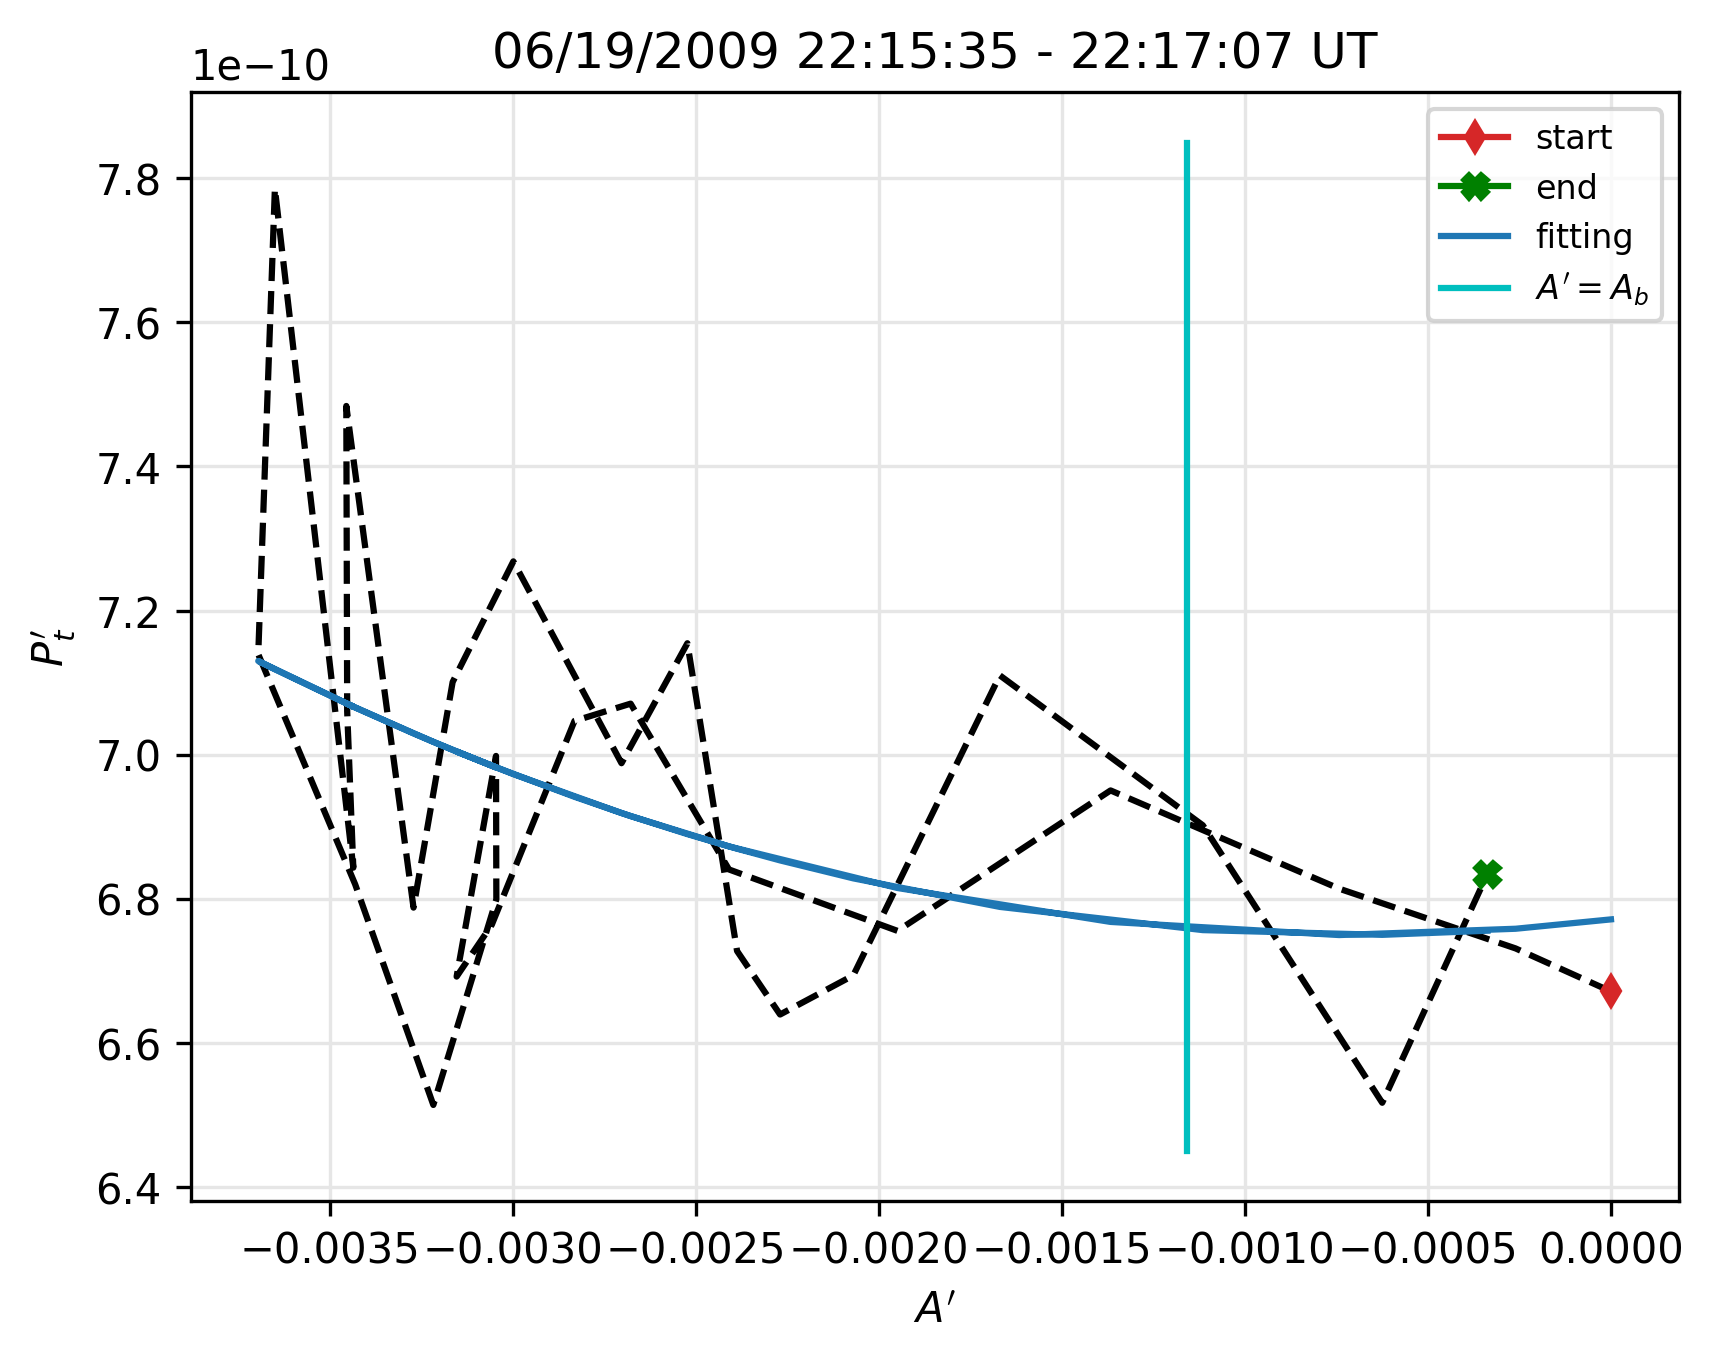
\includegraphics[width=\textwidth]{Figures/Reconstructions/PtvsA_Ab_20090619_20090621.png}
    \caption[Double folding pattern of $P_t'$ versus $A'$ for 22:15:35-22:17:05 UT on 19 June 2009]{$P_t'(A')$ versus $A'$ plot for an SFR from 22:15:35-22:17:05 on 19 June 2009 observed by THM-C. The red and green markers indicate the starting and ending points of the SFR interval, the darker blue line indicates the fitted $P_t'(A')$ versus $A'$ function, and the lighter blue line indicates the turning point where $A'=A_b$.}
    \label{fig:Pt-vs-A-Ab}
\end{figure}

\begin{figure}
    \centering
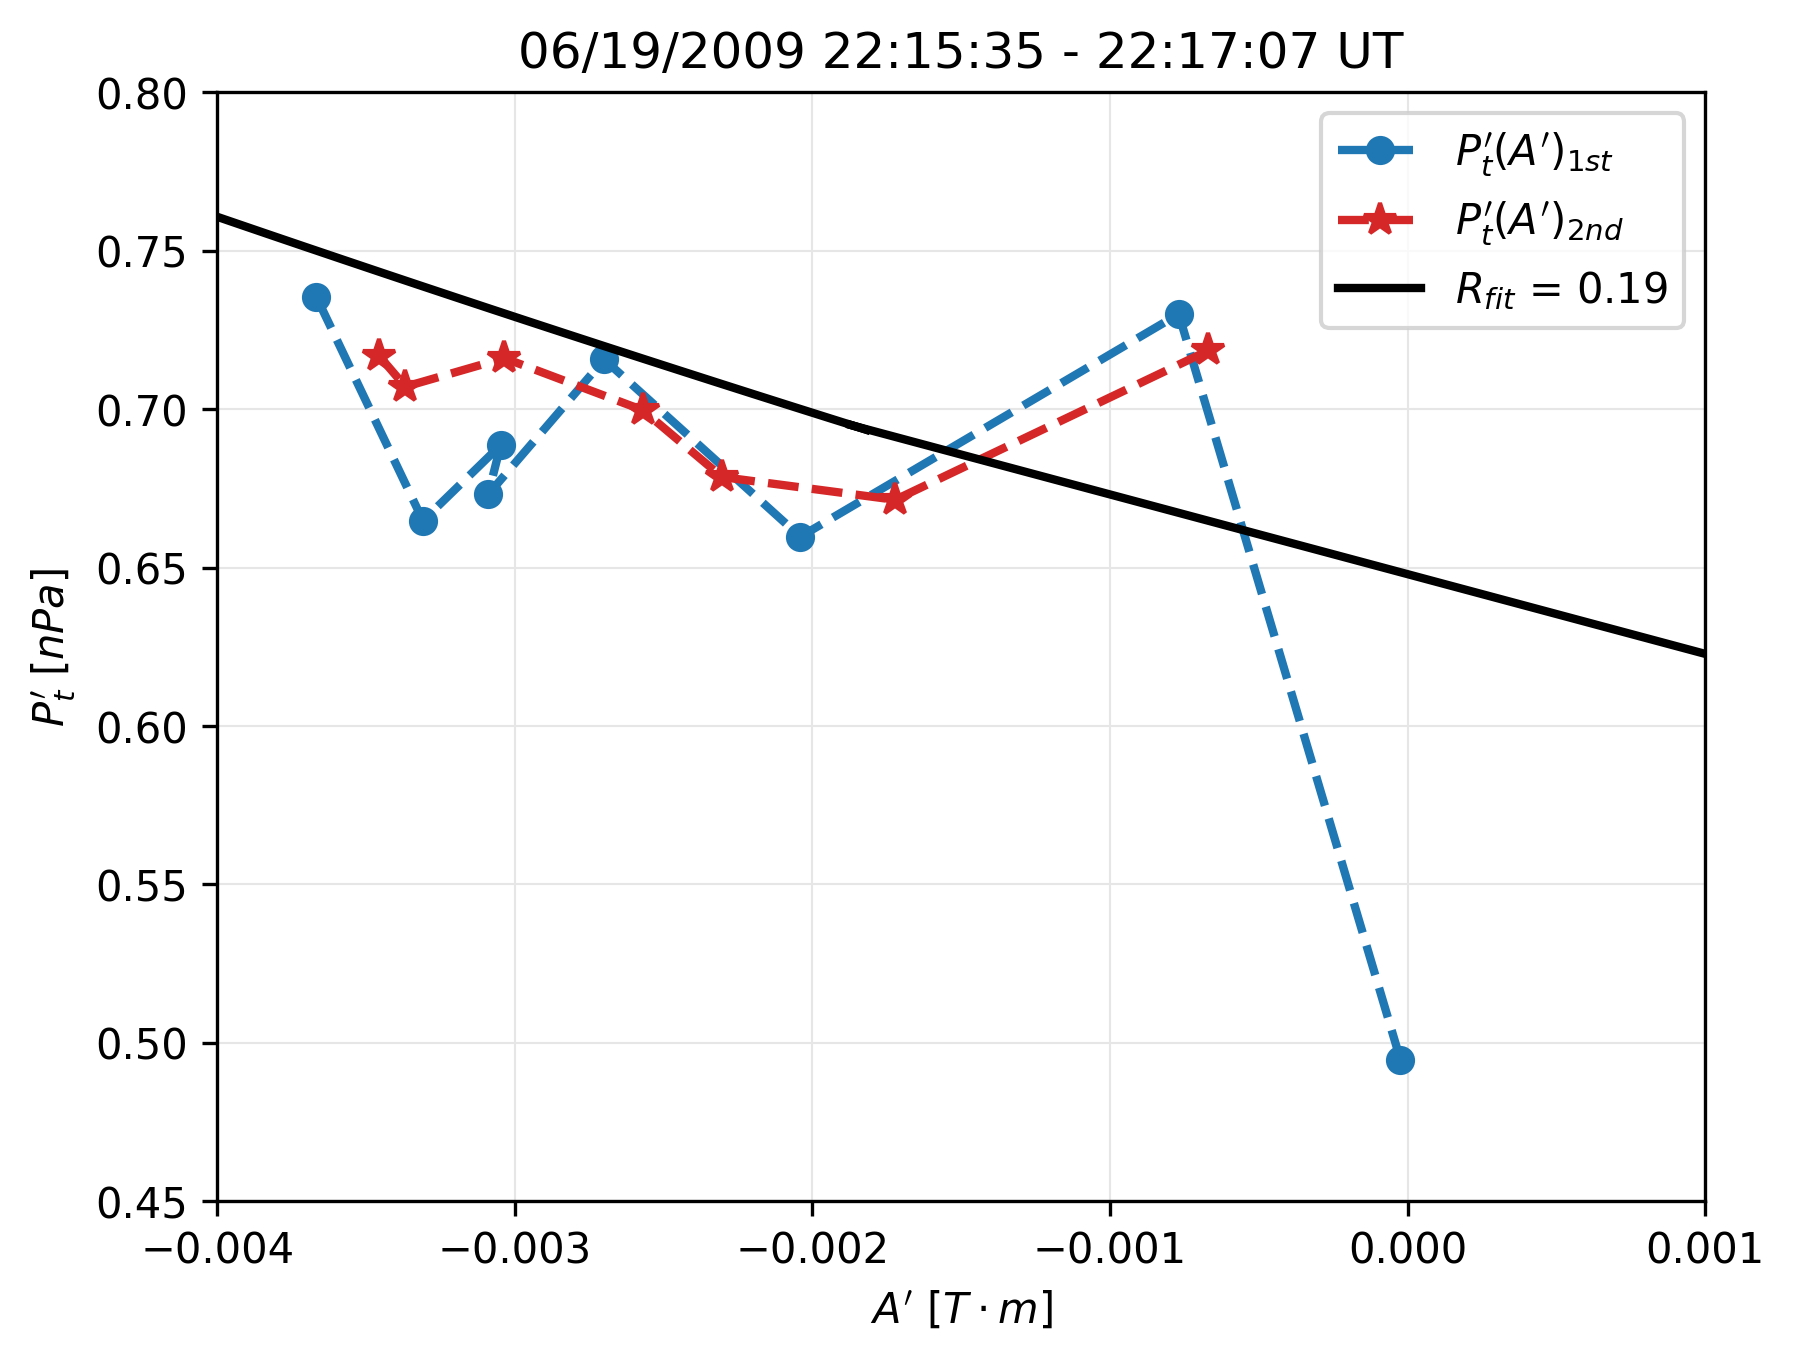
\includegraphics[width=\textwidth]{Figures/Reconstructions/PtvsA_20090619_20090621.png}
    \caption[$P_t'$ versus $A'$ plot for 22:15:35-22:17:05 UT on 19 June 2009]{The $P_t'$ versus $A'$ plot for an SFR interval from 22:15:35-22:17:05 UT on 19 June 2009 observed by THM-C. The data points are marked by the symbols, and are connected by the blue dashed line and the red dashed line, separated by the turning point at the minimum of $A'$ in this case. The two lines correspond to the first and second parts of the $P_t'(A')$ curve as denoted by the legend. The solid black curve represents a functional fitting to the data points with fitting residue $R_{fit}$.}
    \label{fig:Pt-vs-A}
\end{figure}

% The data are then used to calculate the transverse pressure $P_t'(A')$ as a function of the scalar flux function, $A'$. If the $P_t'$ versus $A'$ is double folded through a flux rope interval, then two metrics, $R_{diff}$ (the point-wise difference between the two folds) and $R_{fit}$ (a fitting residue of $P_t'(A')$), are used to check the double-folding quality and the shape of $P_t'(A')$. The threshold values for these metrics are selected empirically to guarantee good flux rope quality \citep{Hu:2018}, and if the thresholds are met, the event is recorded as an event candidate. If the thresholds are not met, the $z$-axis will go through its next iteration until the thresholds are met.

After the initial detection of SFR candidates, the list of initial candidates is refined. The records are further classified based on the Wal\'en test slope $w$. Records with $|w|\leq0.3$ are quasi-static SFRs and thus saved directly. Records with $|w|>0.3$, except for when the correlation coefficient $r$ between the aforementioned two velocities ($\mathbf{V_{sw}} - \mathbf{V_{HT}}$ and $\mathbf{V_A}$) is $|r|\geq 0.8$ and $\langle M_A\rangle \leq 0.9$, are removed. These conditions ensure that the remaining plasma flow is aligned with the local magnetic field, and also to avoid a singularity in Equation (\ref{eq:GSextended}) at $\alpha=1$. Events with $\alpha>1$ are rare, but they are also removed, so that the events remaining are sub-Alfv\'enic. We also remove events from the initial candidate list if the candidates have a turning point within $5\Delta t$ (turn time) of the turning point of another candidate with a smaller $R_{diff}$, as these could be the same overlapping structures. Table \ref{tab:thresholds} lays out the threshold conditions as utilized in the post-processing of the GS-based detection event list \cite{Chen:2020, Chen:2021, Chen:2022}. The duration of the search windows does not exceed 343$\Delta t$ ($\sim 25.733$ minutes for MMS and $\sim 24.553$ minutes for THEMIS) due to computational time constraints. The detection algorithm was performed for some time periods with search window size up to 388 points in duration; however, the search yielded very few (generally less than 3) additional event counts after the post-processing steps. This was due to the step of making sure there is no overlap between SFR candidates, which prioritizes smaller duration candidates. Therefore, with the search algorithm taking a significant amount of time to run for longer search windows and yielding very few results, it was decided to stop the search at the maximum window size of $343\Delta t$. The PyGS software used to reconstruct the 2D cross-section of the events can be found at \url{https://github.com/PyGSDR/PyGS}.
\begin{table}[h!]
\centering
\caption[Threshold conditions for GS algorithm]{Table of threshold conditions for GS reconstruction-based algorithm. $R_{diff}$ and $R_{fit}$ are residues which ensure good double-folding quality in the $P_t'(A')$ vs. $A'$ curve..} %Events meeting the following criteria are kept.} %Duration is $10*dt\sim 343*dt$ where $dt\sim 3$ seconds.
\begin{tabular}{ccccccc}
\toprule
    Duration  & $R_{diff}$ & $R_{fit}$ & Turn time & Wal\'en test slope & $|r|$ & $\langle M_A\rangle$ \\ 
    \hline
    %$\sim$ 30-1029 & $<0.2$ & $<0.2$ & 5$dt$ & $\leq 1$ &  &  \\
    10$\Delta t$-342$\Delta t$ & $<0.2$ & $<0.2$ & 5$\Delta t$ & $|k|\leq 0.3$ & & \\
    10$\Delta t$-342$\Delta t$ & $<0.2$ & $<0.2$ & 5$\Delta t$ & $|k|> 0.3$ & $\geq 0.8$ & $\leq 0.9$ \\
\bottomrule %30-1029 (s)
\end{tabular}
\label{tab:thresholds}
\end{table}

%Solar wind
%k <= 0.3:  1752
%k > 0.3; r>|0.8|, <M_A> <0.9:  107

% Magnetosheath
%k <= 0.3:  2310
%k > 0.3; r>|0.8|, <M_A> <0.9:  70


\begin{figure}
    \centering
    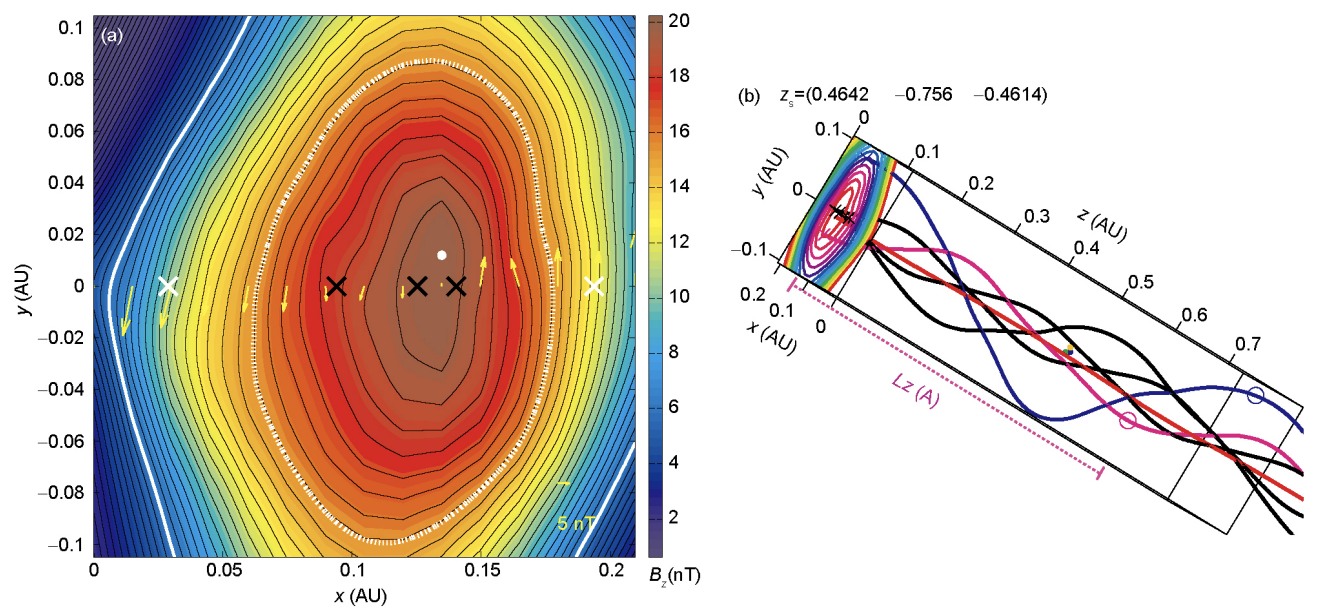
\includegraphics[width=\textwidth]{Figures/Reconstructions/Hu2015_GSreconstruction.png}
    \caption[GS 2D reconstruction of a magnetic cloud]{Reconstruction of a magnetic cloud \citep{Hu:2015}: a) 2D cross section of $A(x,y)$ for a reconstructed magnetic cloud event. The black lines indicate the transverse magnetic field lines, and the color bar indicates the axial field lines $B_z$. The yellow arrows denote the transverse field lines ($B_t$) along the path of the spacecraft ($y=0$). The white contour indicates the area of the reconstruction done from spacecraft data ($A=A_b$), while the area outside the white contour is reconstructed from extrapolation. b) 3D view of a flux rope structure for the magnetic cloud event, showing the 2D cross section (A') and selected associated twisted magnetic field lines along the flux rope axis (denoted at the top). The black field lines  rooted at the foot points where the electron onsets were observed. The pink and blue circles denote the locations where the associated field lines complete a full turn around the z-axis.}
    \label{fig:GSreconstruction_Hu2015}
\end{figure}

%Such an extended version searches FRs including those with significant field-aligned flows as they also meet the broad definition of magnetic flux ropes, \textit{i.e}., having twisted field lines around the central axis \citep{Chen:2021}. Therefore, the Alfv\'enicity of these dynamic structures is not negligible, which will be characterized by the $M_A$ and the Wal\'en test slope.

\section{Wal\'en test and Alfv\'enicity}
The Wal\'en test slope $w$, the slope of the linear regression between $\mathbf{V_{sw}} - \mathbf{V_{HT}}$ and $\mathbf{V_A}$, is then used to further distinguish Alfv\'enic structures

%generalized test is most simply formulated as a vector difference equation relating changes in the electron velocity vector and changes of the magnetic field vector, with a prescribed scalar constant of proportionality.

\section{Analysis results}
\begin{figure}
    \centering
    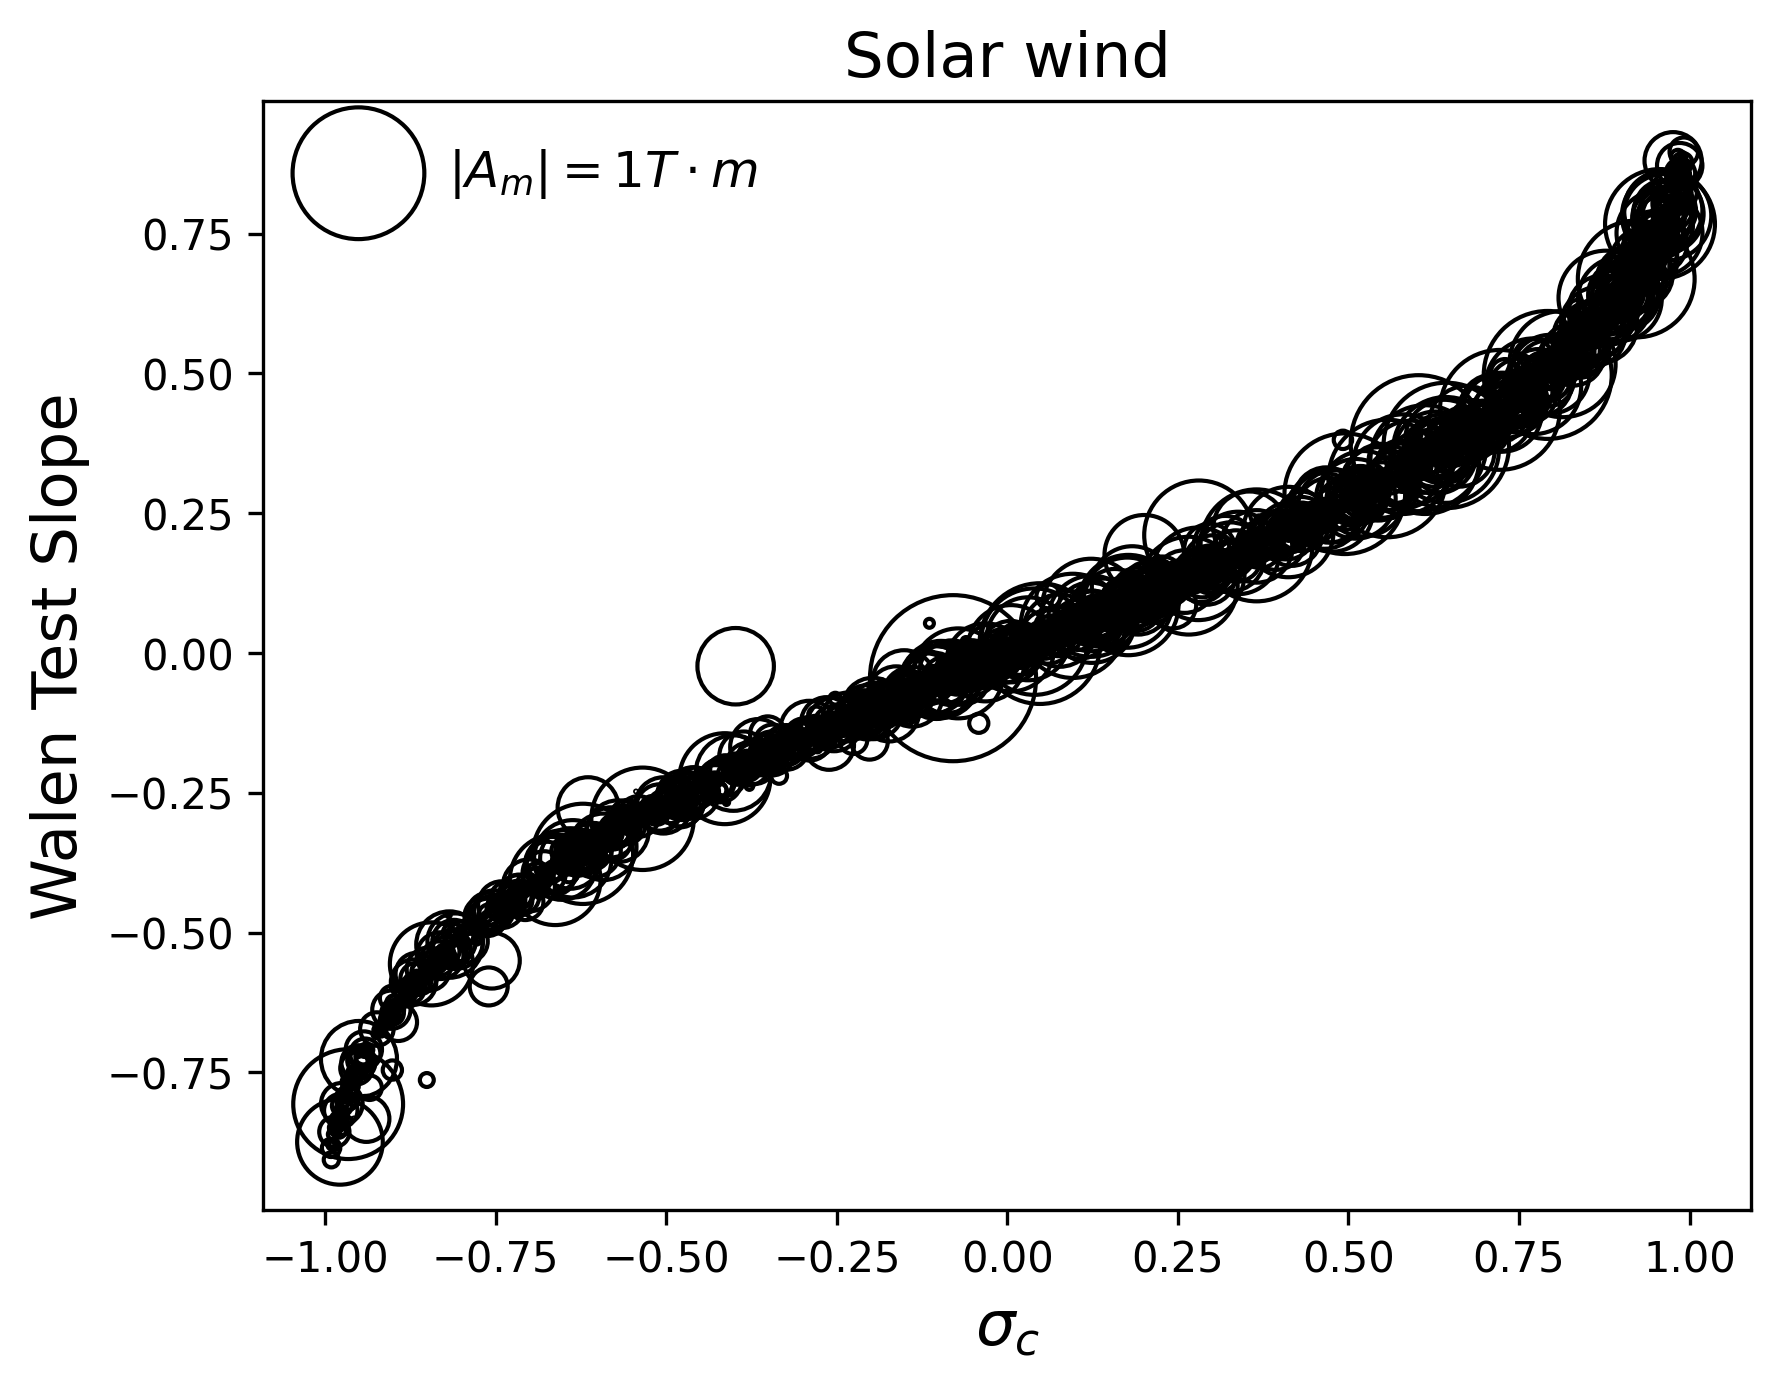
\includegraphics[width=0.45\linewidth]{Figures/GS analysis/walenTest_vs_crosshelicity_solarwind.png}
    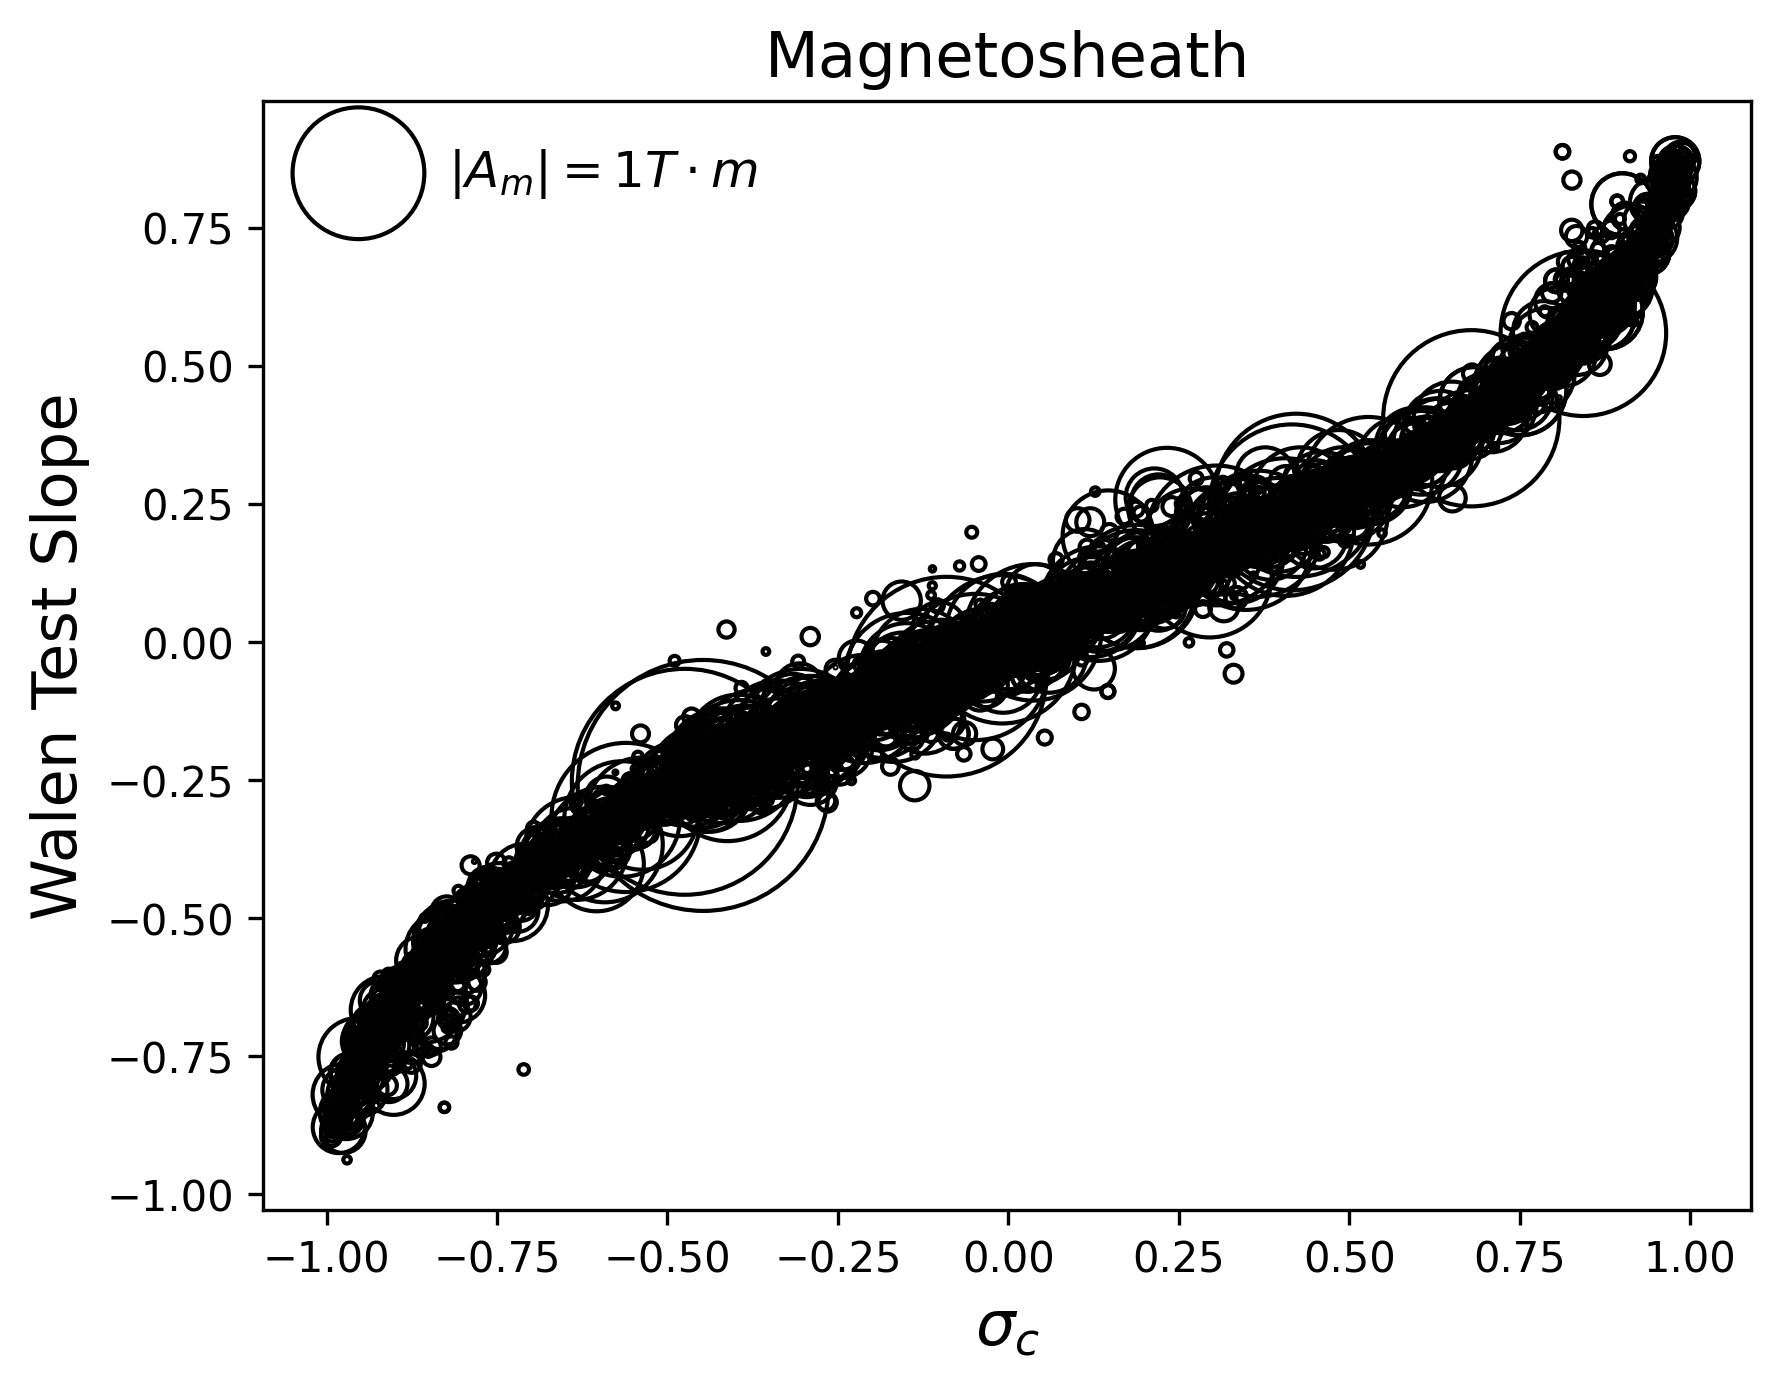
\includegraphics[width=0.45\linewidth]{Figures/GS analysis/walenTest_vs_crosshelicity_magnetosheath.png}
    \caption[Wal\'en test slope vs. reduced cross helicity]{Caption}
    \label{fig:walen-crosshelicity}
\end{figure}


\begin{figure}
    \centering
    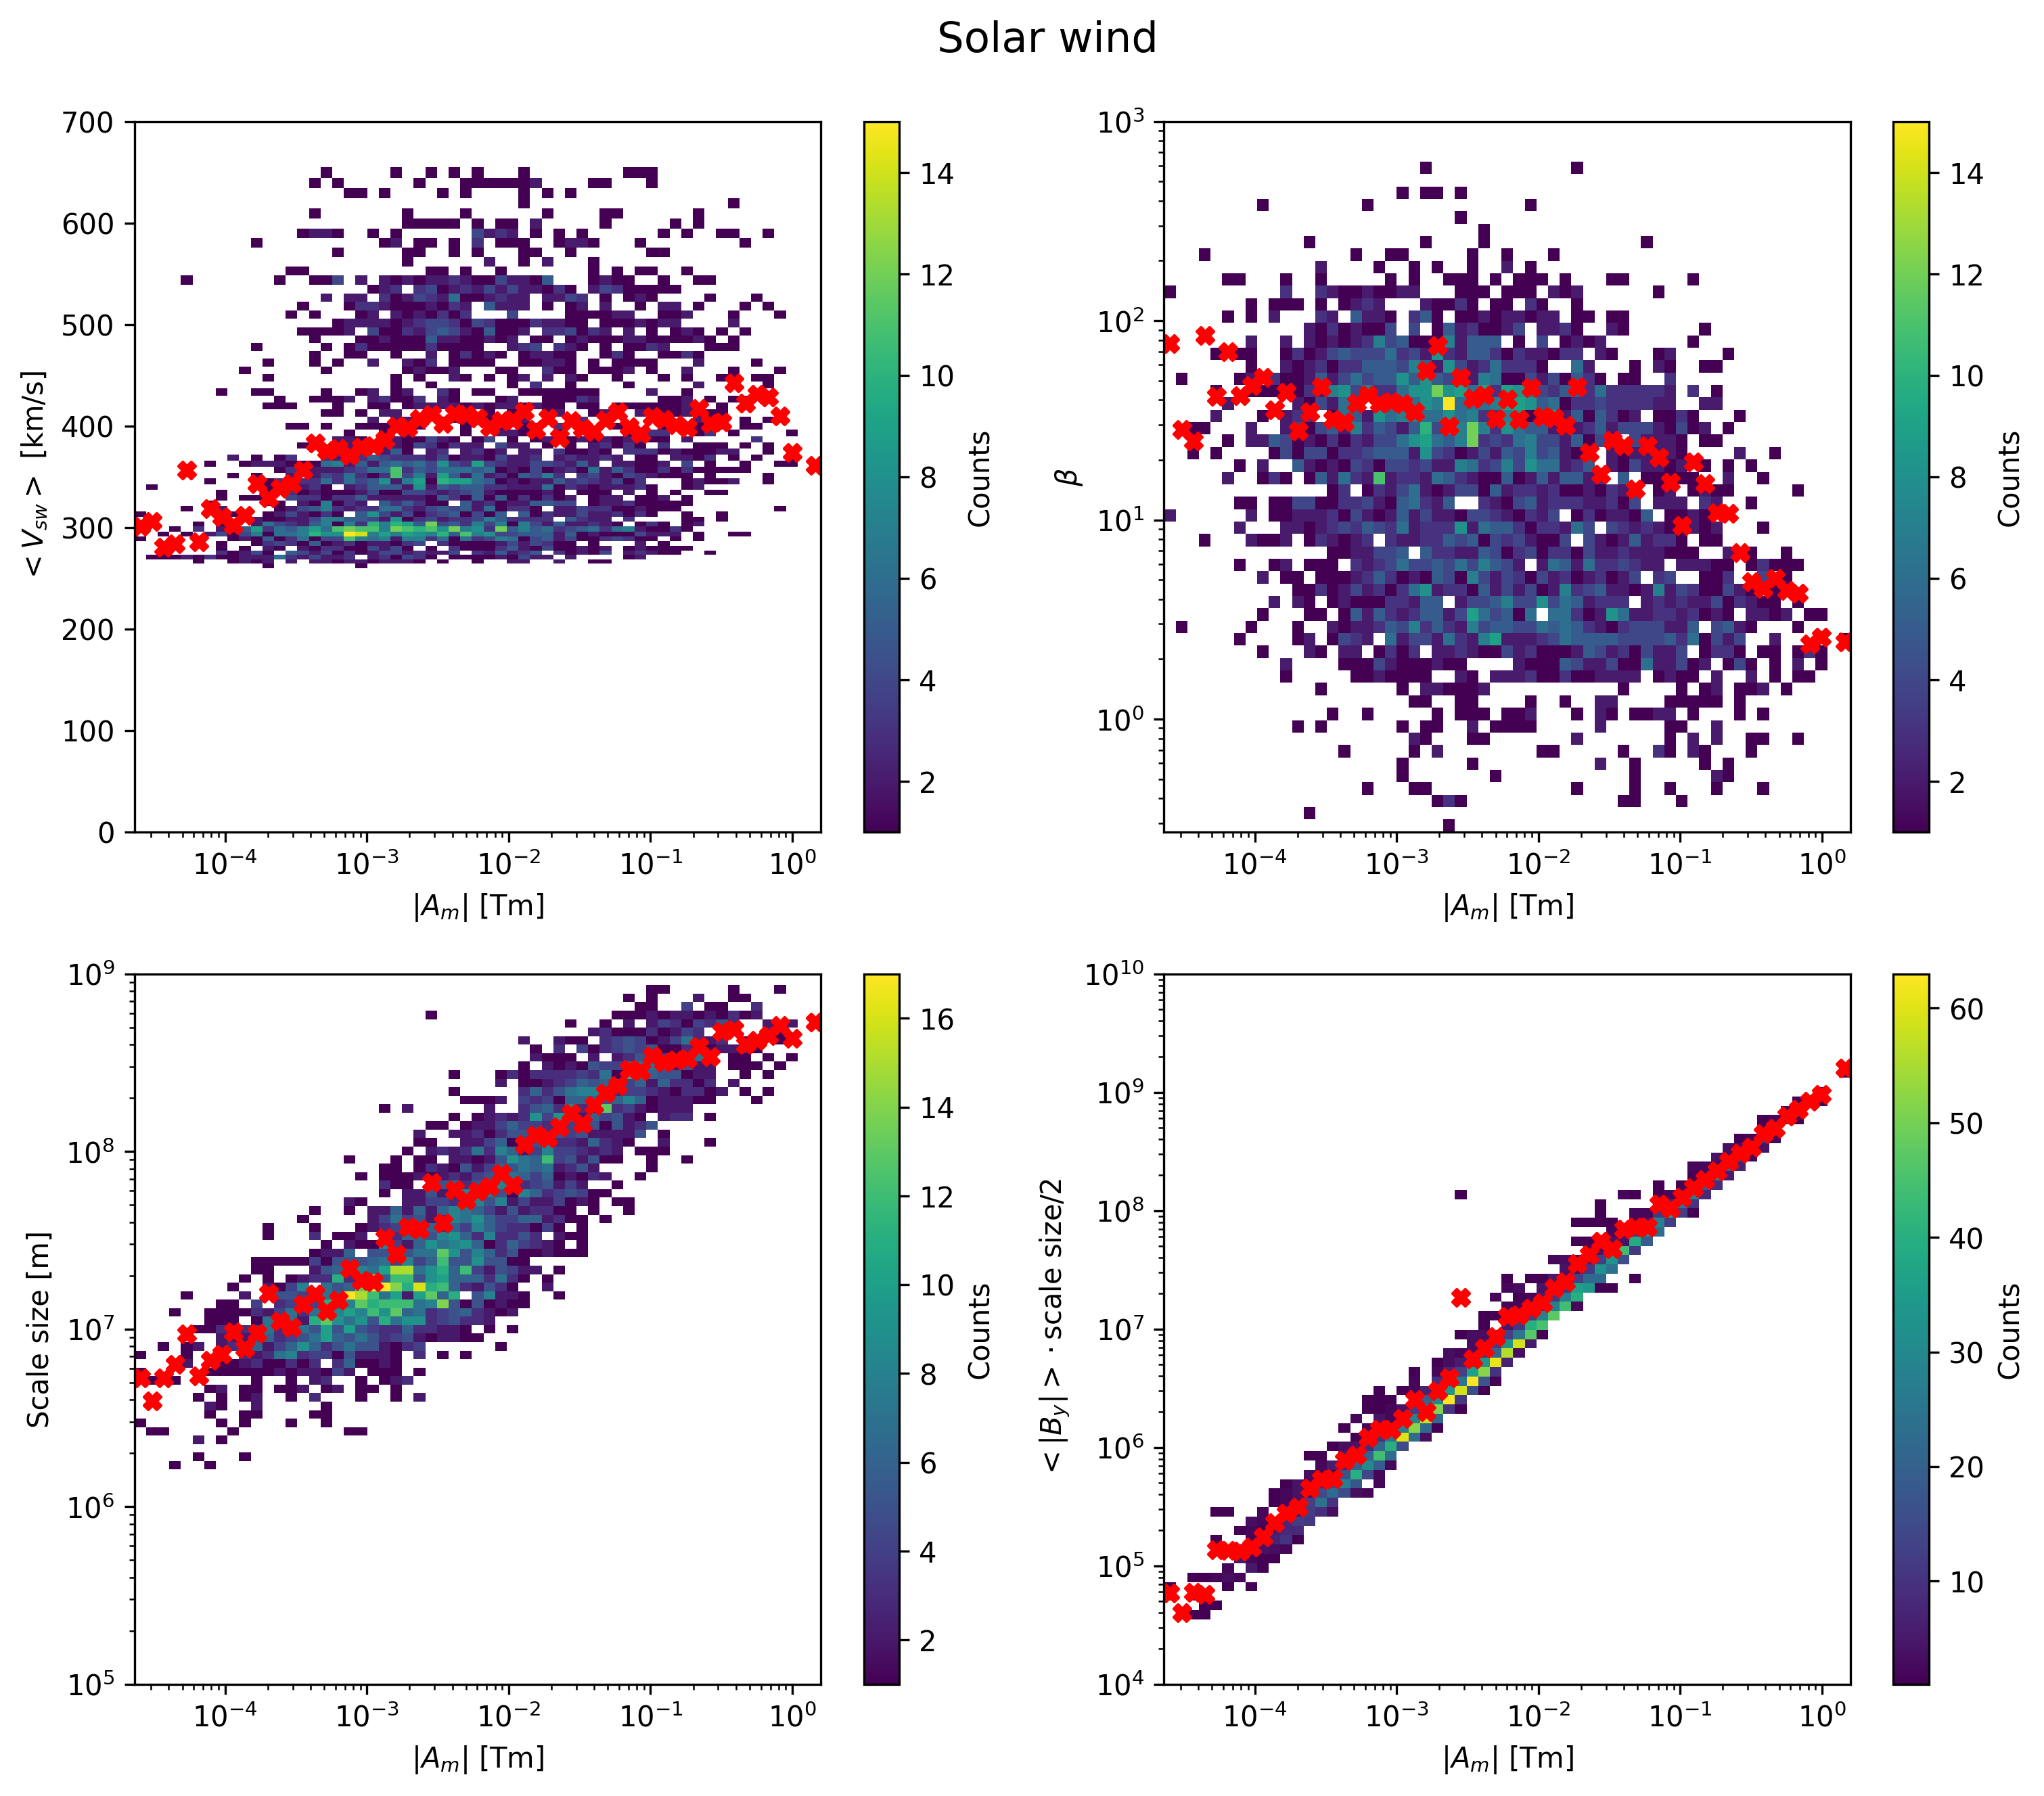
\includegraphics[width=0.45\linewidth]{Figures/GS analysis/heatmap_solarwind.png}
    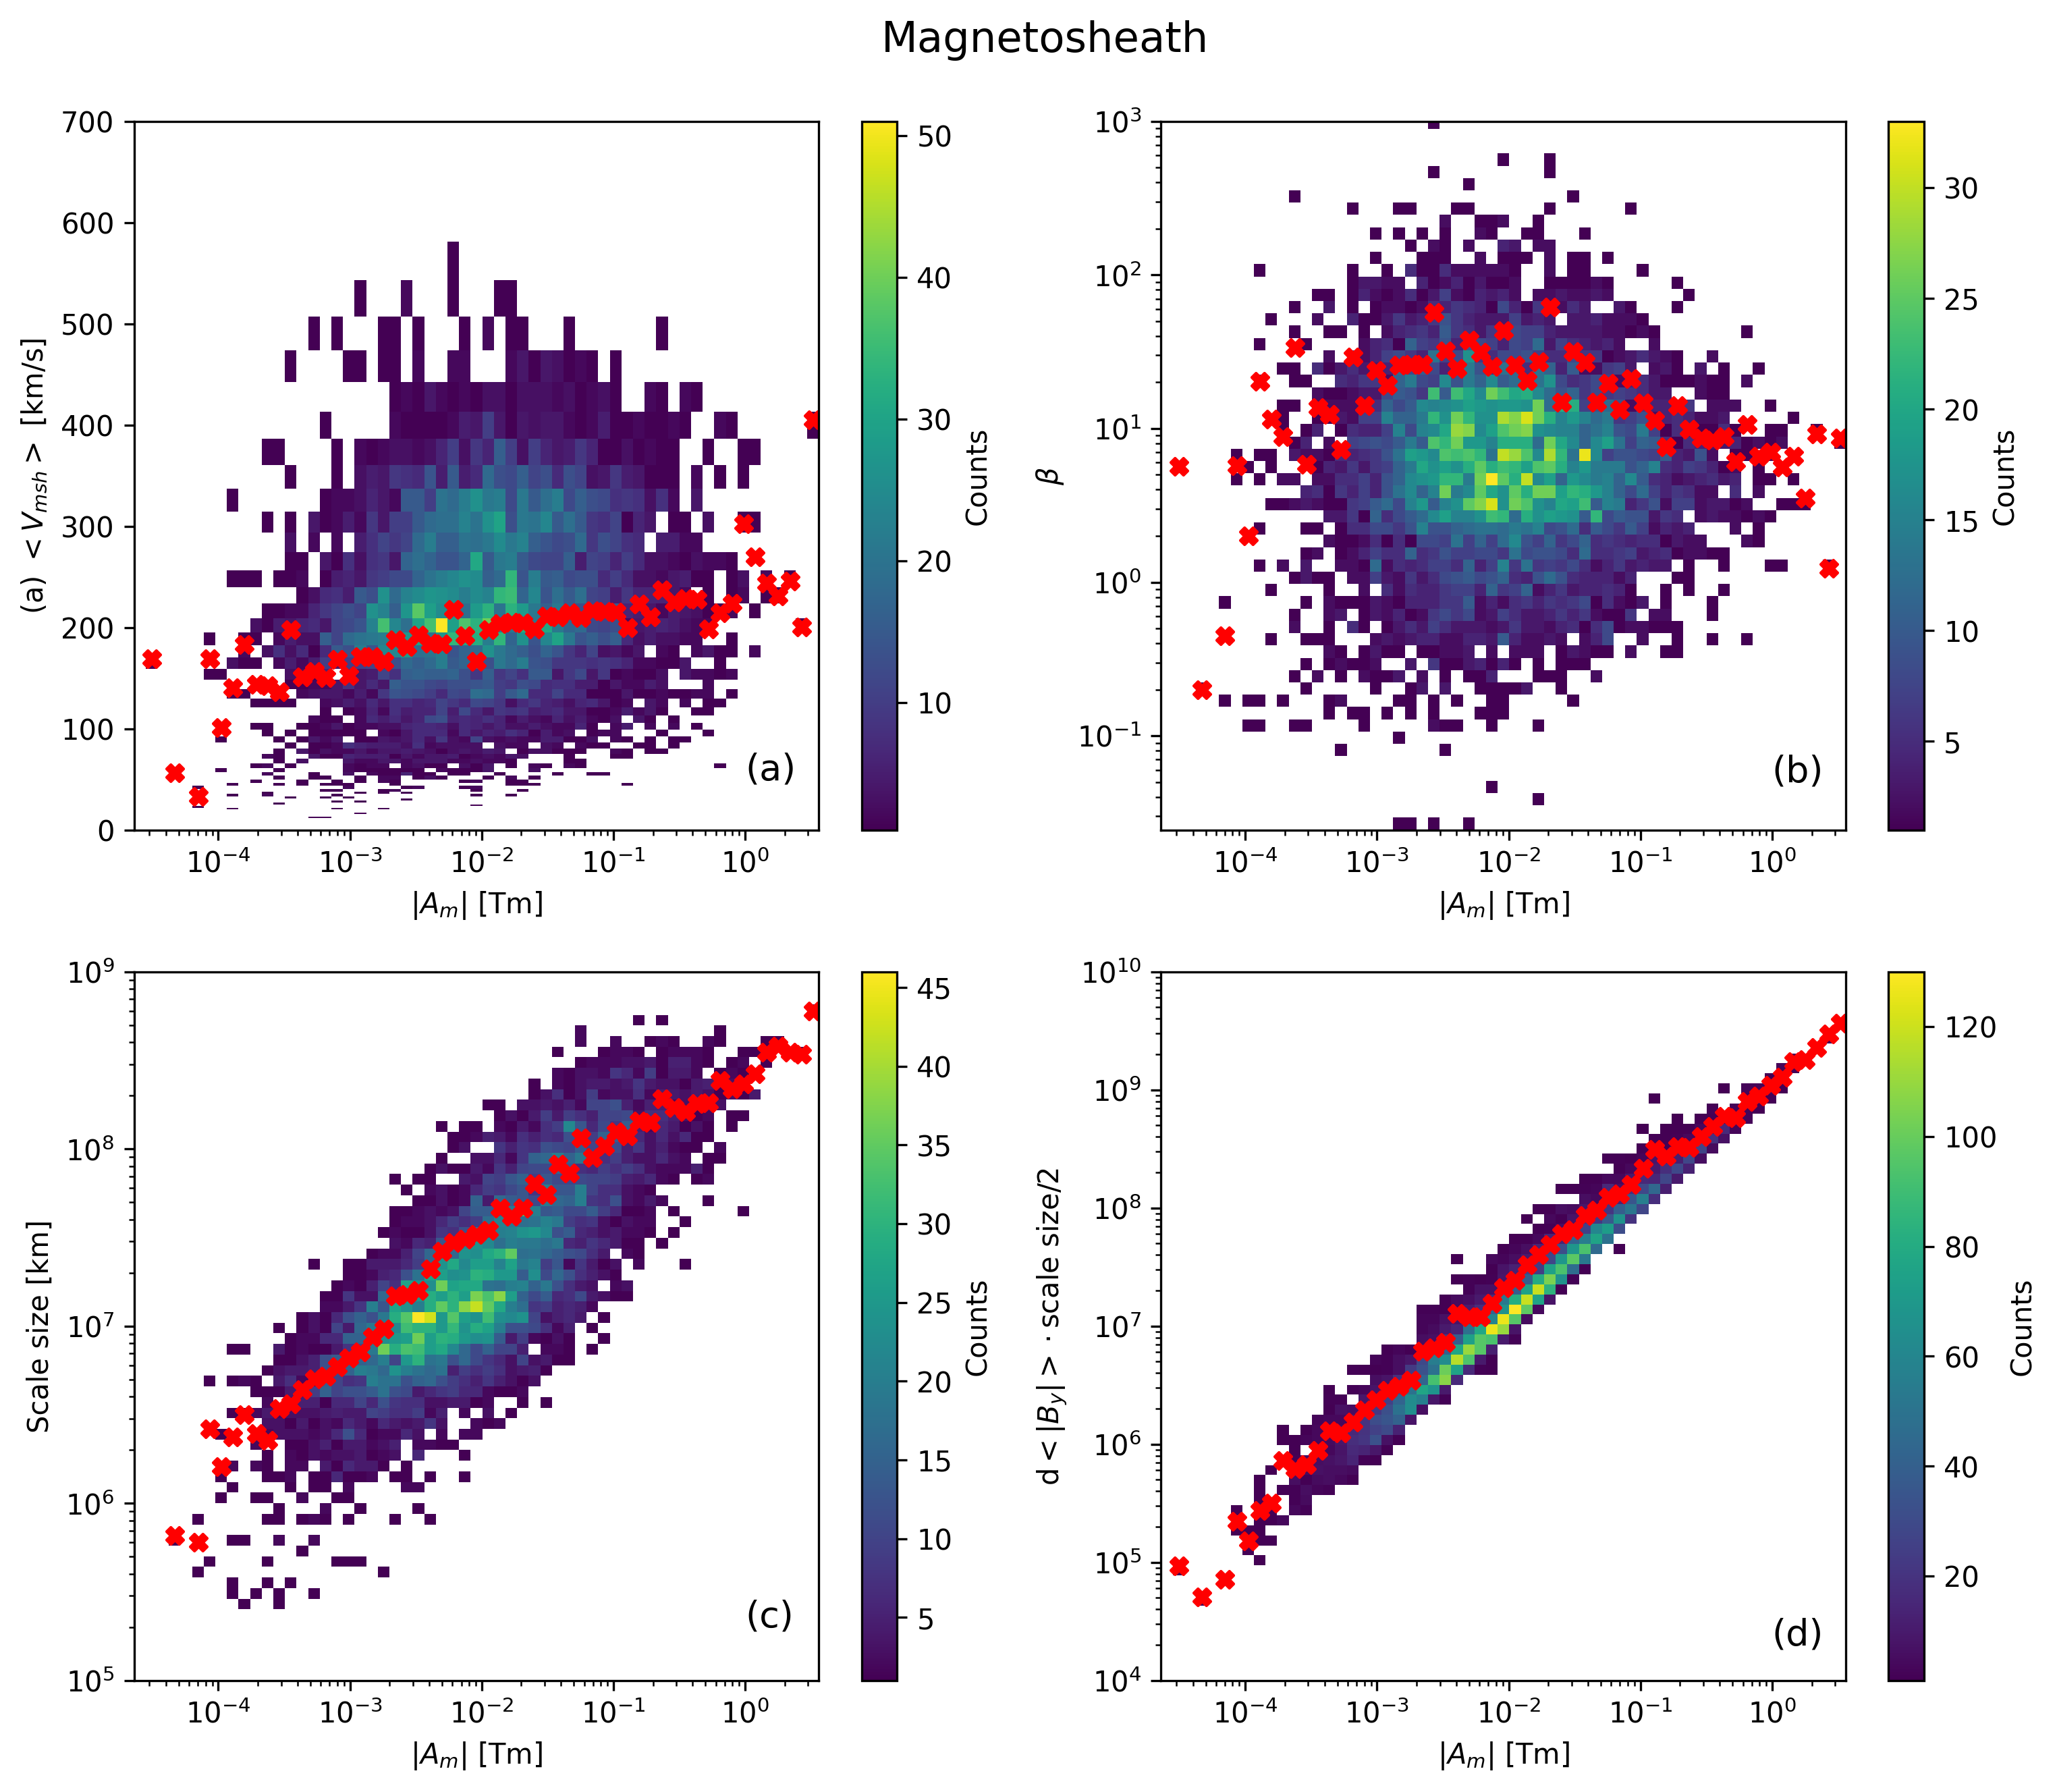
\includegraphics[width=0.45\linewidth]{Figures/GS analysis/heatmap_magnetosheath.png}
    \caption[2D distributions of various parameters vs. $|A_m|$]{Caption}
    \label{fig:heatmap-A}
\end{figure}
\chapter{Chapter 5. Coordinated Analysis}
As a subsection of the analysis, a coordinated analysis between the magnetosheath and solar wind over $\sim$250 hours was performed in order to compare simultaneous observations.  The dayside science and radiation belt science phases of the THEMIS mission offer optimal configuration for direct comparison of the near-Earth solar wind and magnetosphere, specifically those in 2008, 2009, 2018, and 2022. MMS is also used in conjunction with the THEMIS probes for the time periods identified in 2022. 19 time intervals were identified during these phases for which there were simultaneous measurements by two THEMIS probes, where one was in the solar wind and one was in the magnetosheath. For the 2022 orbit phase, MMS-1 data was included for its respective region. It should be noted that the data came from simultaneous measurement in two regions during the same interval, \textit{not} a measurement across the bow shock. 

\begin{figure}
    \centering
    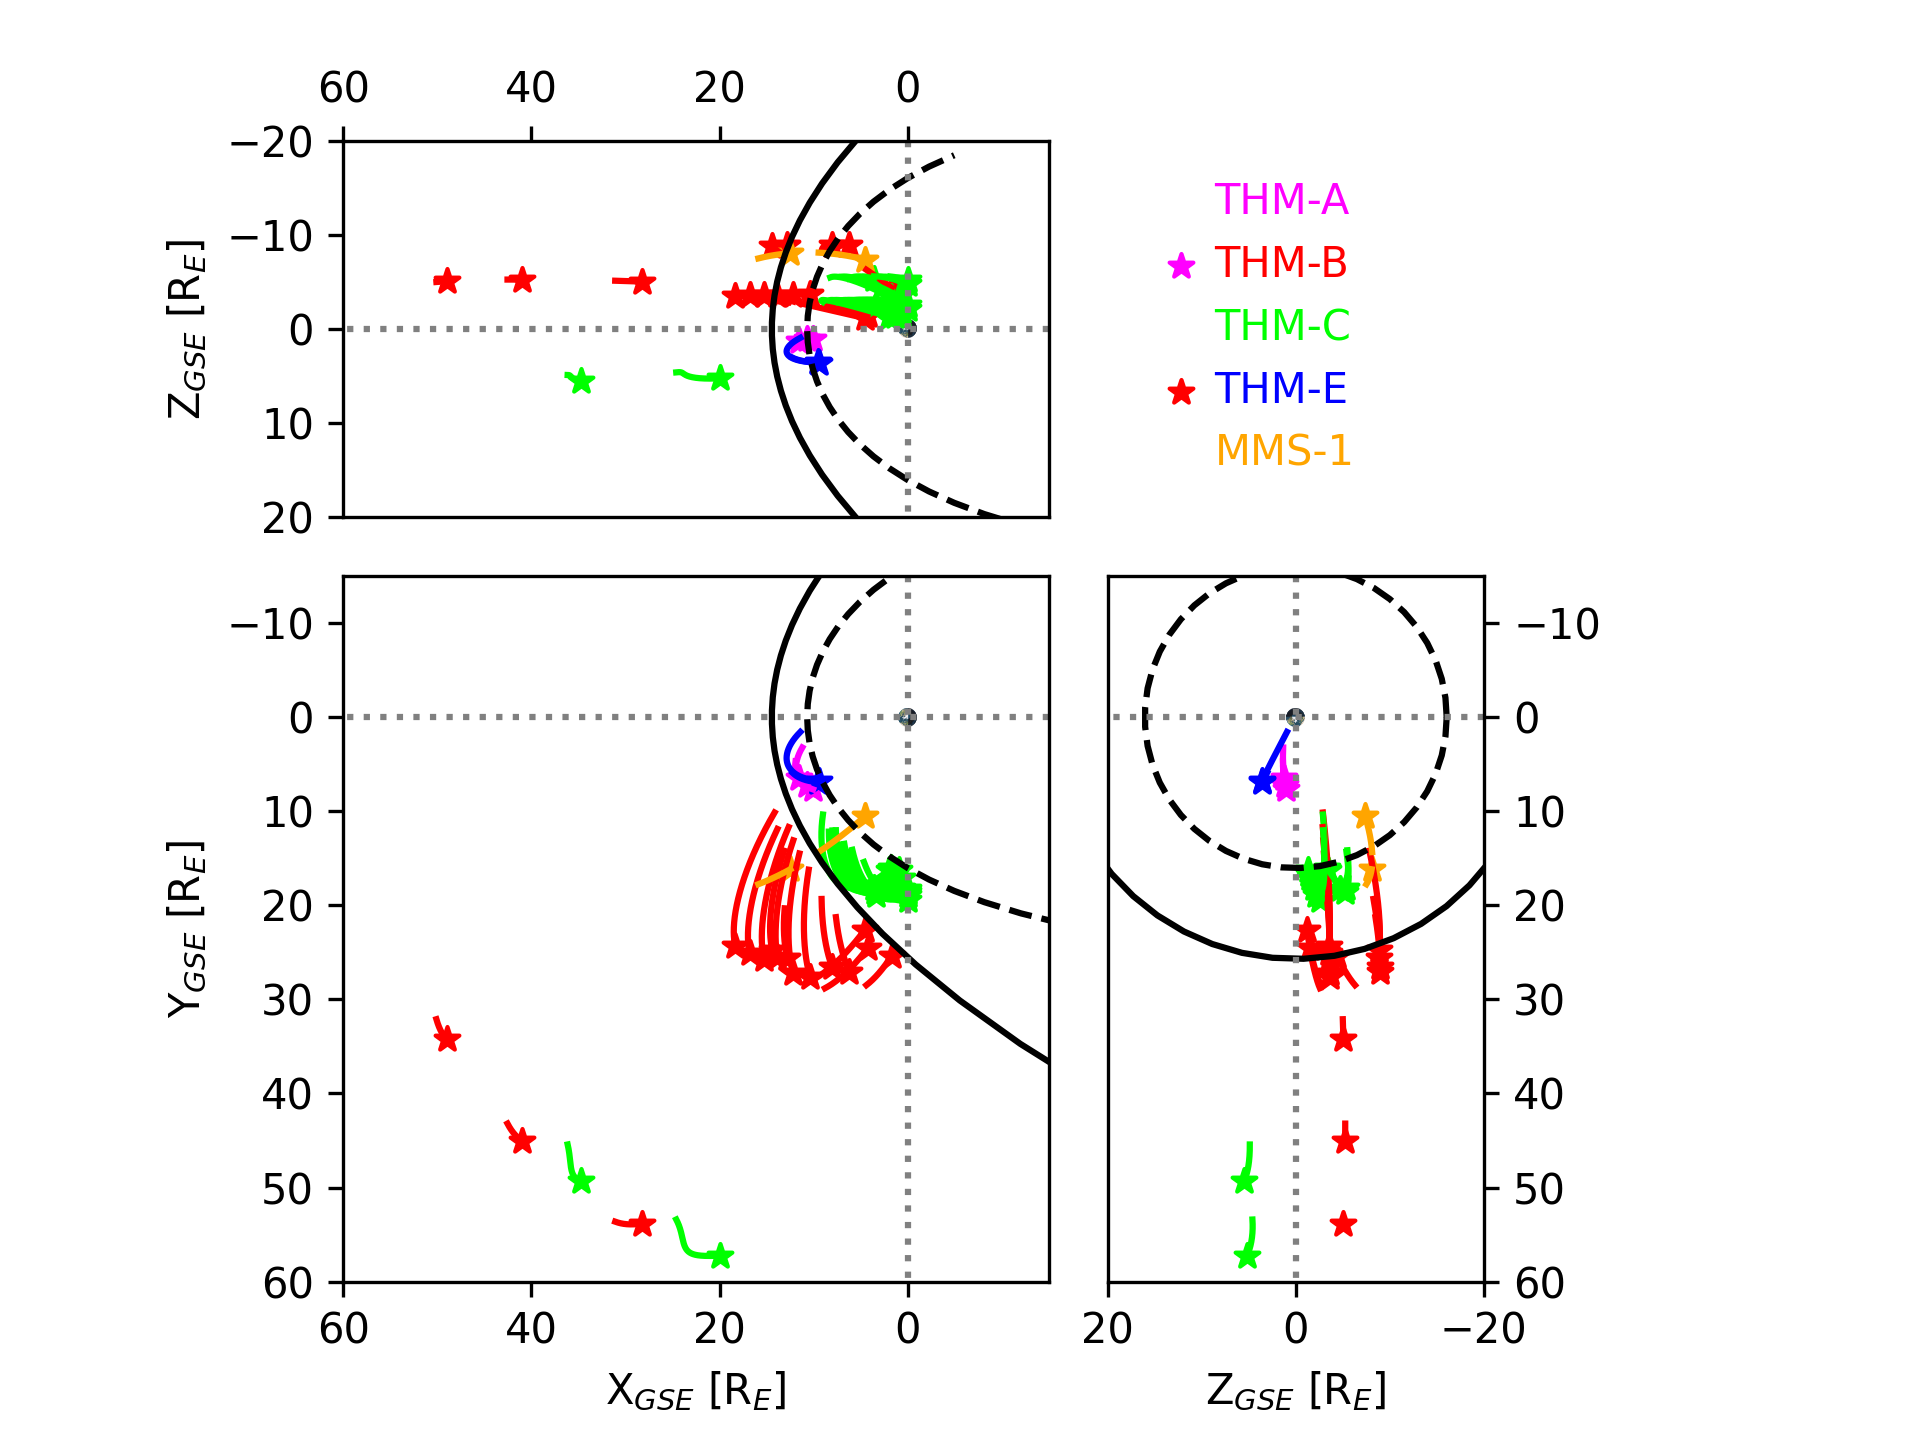
\includegraphics[width=\textwidth]{Figures/Orbits/all_TE_orbits_xy_xz_yz_coordinated.png}
    \caption[Orbits for coordinated observation periods]{Orbits for coordinated analysis time periods are shown in the Geocentric Solar Ecliptic (GSE) coordinates for THEMIS probes A, B, C, and E (THM-A, THM-B, THM-C, THM-E) and MMS-1 probe (see legend), with the stars marking the end of each orbit period. The approximate nominal locations of the magnetopause (dashed black line) modeled using the \cite{Shue:1997} model and bow shock (solid black line) modeled using \cite{SlavinHolzer:1984} are shown, based on the IMF data obtained for one period in 2015 only.}
    \label{fig:coordinated-orbits-plot}
\end{figure}


Figure \ref{fig:timeseries-THM-magnetosheath} is an example of one of the time periods observed in the magnetosheath during the coordinated analysis. These measurements were taken in the magnetosheath with THM-C, while the measurements in the solar wind were taken with THM-B. Following the same procedures as outlined in Section \ref{sec:wavelet-algorithm}, 3308 structures were identified in the solar wind, and 3446 structures were identified in the magnetosheath during the coordinated intervals. The reconstruction in Figure \ref{fig:reconstruction-June2009} shows a flux rope reconstruction during this interval. 

\begin{figure}
    \centering
    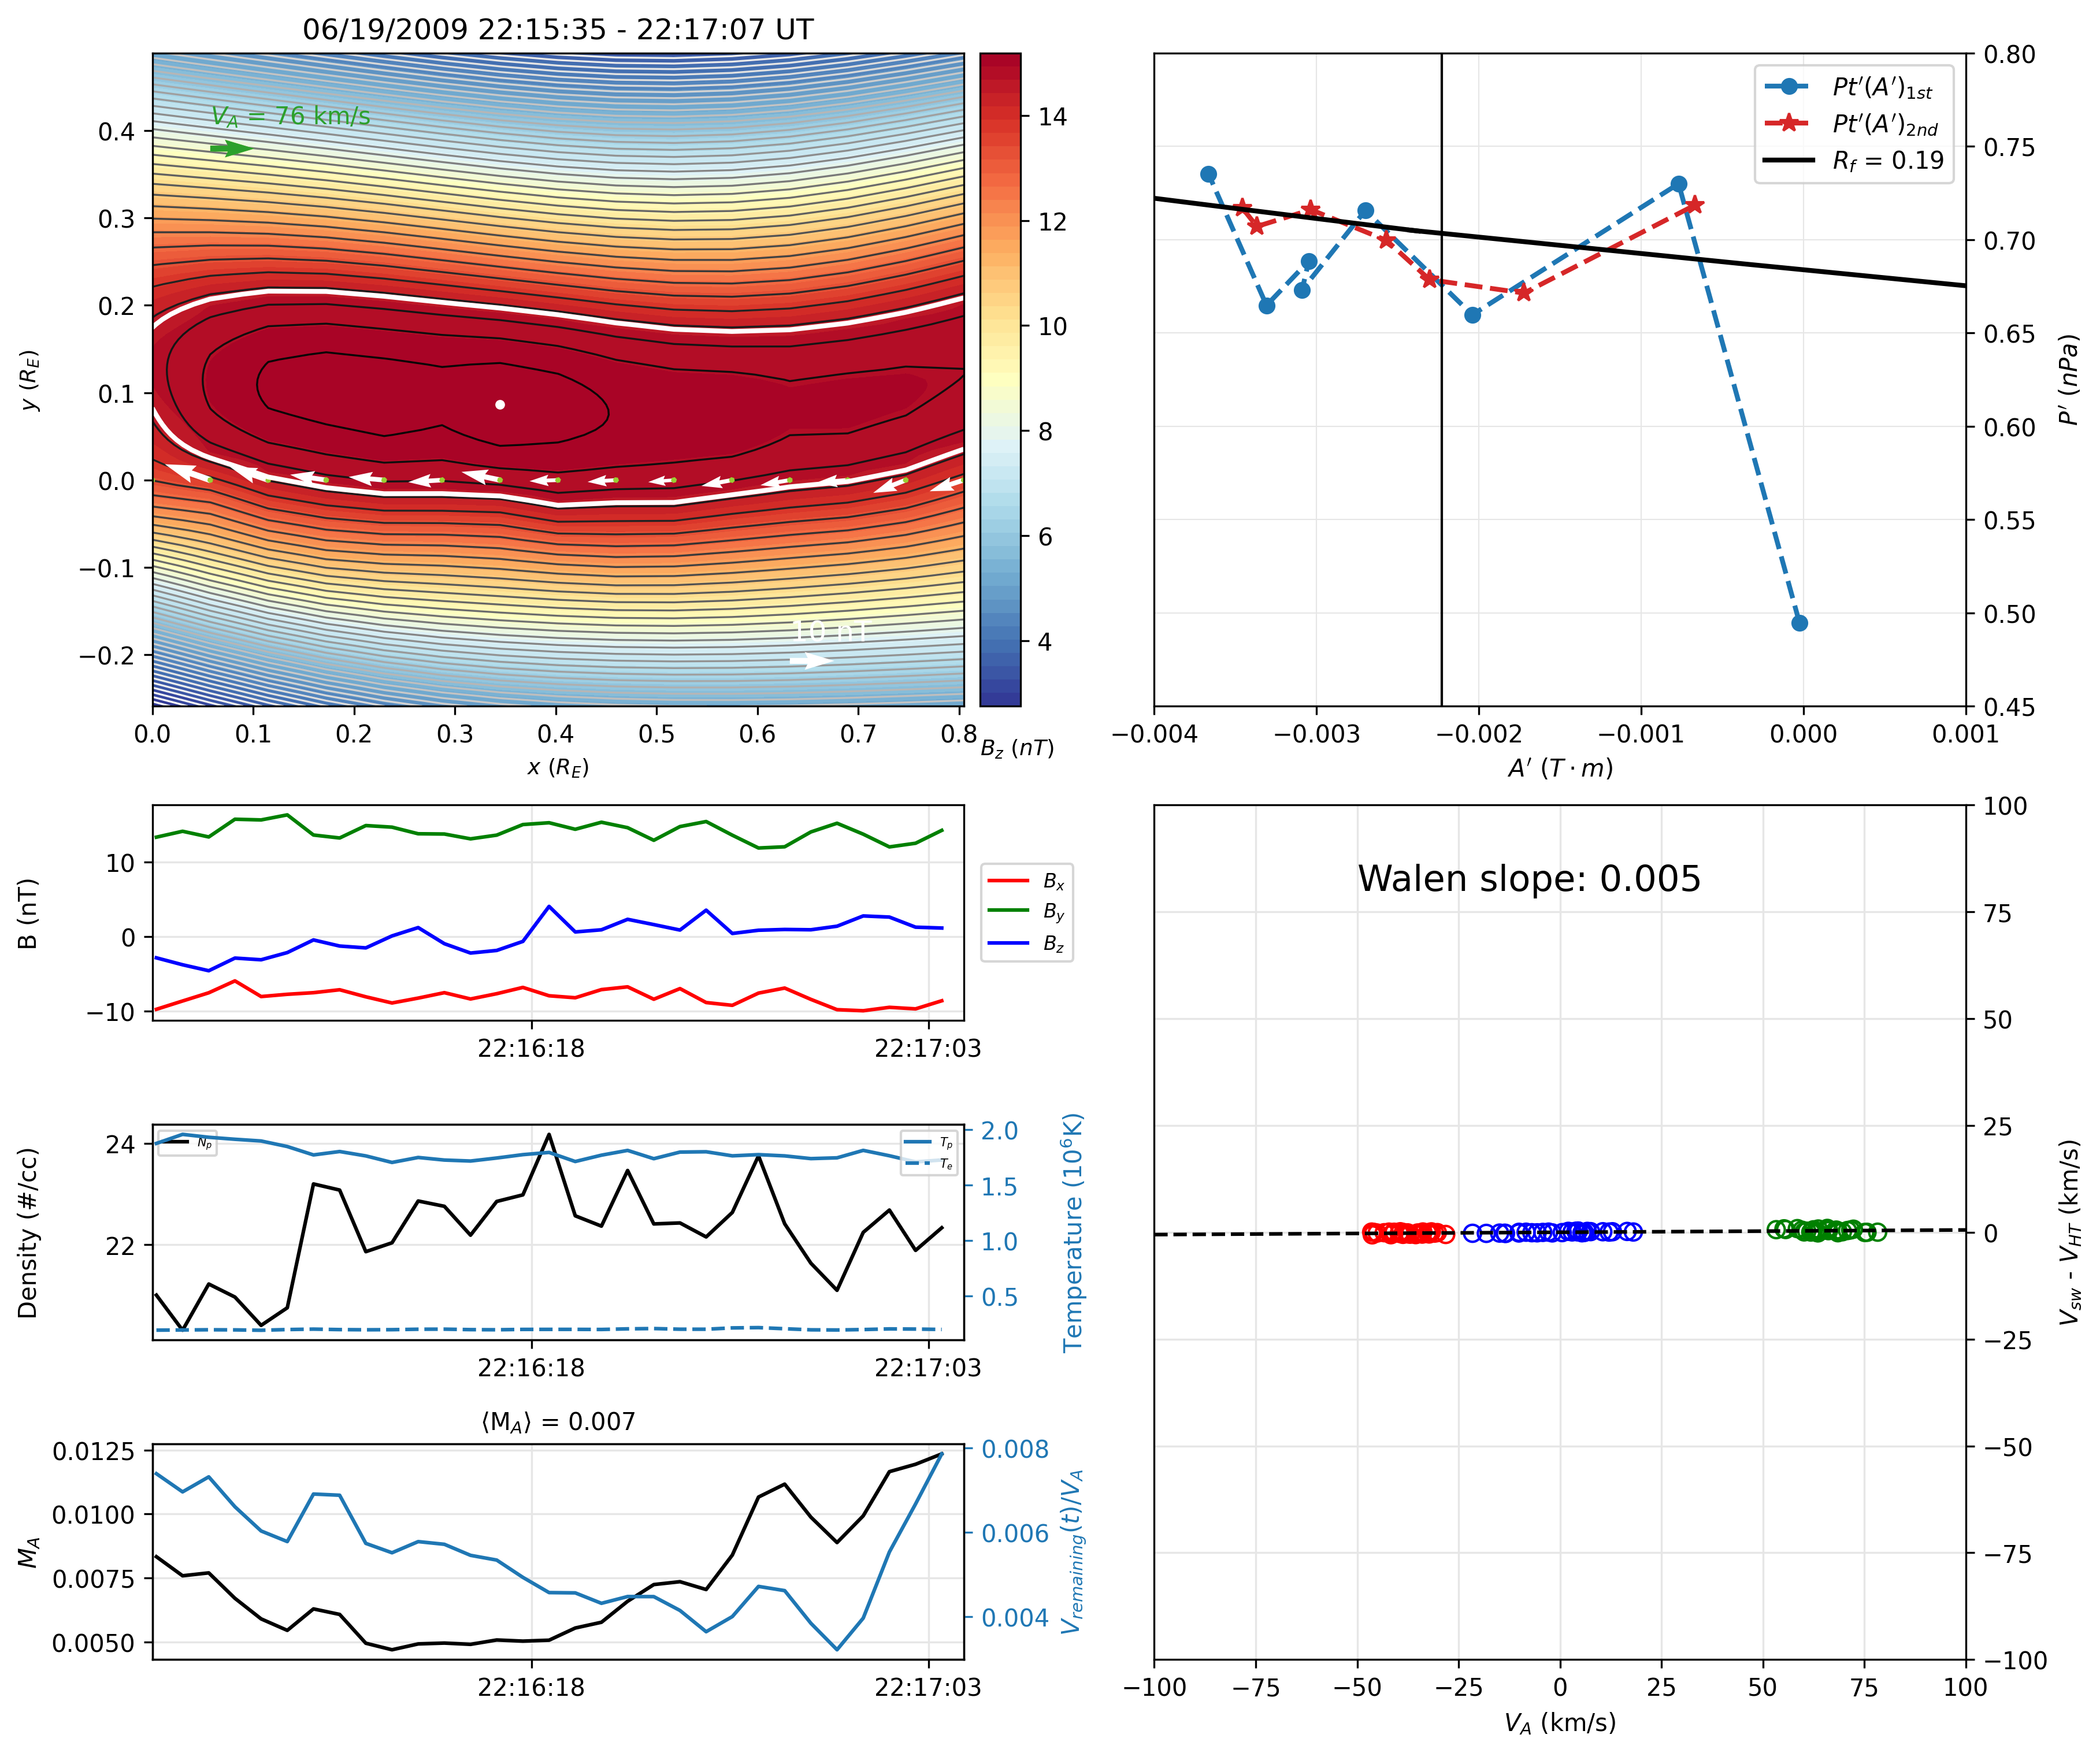
\includegraphics[width=\textwidth]{Figures/Reconstructions/timeseries_walenTest_20090619_20090621.png}
    \caption[GS event reconstruction]{GS-based reconstruction of an event from 22:15:35-22:17:07 UT on 19 June 2009. Top left: 2D cross-section, with $\hat{x}_{GSE}=[0.761, -0.103, 0.640]$, $\hat{y}_{GSE}=[0.628, 0.365, -0.688]$, $\hat{z}_{GSE}=[-0.163,0.925,0.342]$. Bottom left: Associated time series data for THM-C in the magnetosheath during this period. Top right: $P_t'(A')$ vs. $A'$ curve for this event. Bottom right: Wal\'en relation for this event.}
    \label{fig:reconstruction-June2009}
\end{figure}


Table \ref{tab:coordinated-summary} displays the results for the number of events identified with each method. Table \ref{tab:coordinated-MHD-Walen} shows the characterization of the events for each method according to MHD criteria (wavelet analysis) and Wal\'en slope (GS reconstruction).

% summary table
\begin{table}
    \centering
    \caption{Summary table for events identified via wavelet analysis and the GS reconstruction algorithm}
    \begin{tabular}{rcccccc}
\hline
Region                    &  Method &  \# Events &  Avg. duration &  Avg. B &  Avg. scale \\
 &    &   &  [mins] &  [nT] &  size [km] \\
\hline
         	         & Wavelet & 1407 & 6.43 & 3.93  & 1.4$\times 10^5$ \\
\textit{Solar wind} 	  & GS 	    & 1901 & 3.46 & 3.90  & 6.0$\times 10^4$ \\
         	           & Total   & 3308 & 4.72 & 3.91  & 9.3$\times 10^4$ \\
\hline
         	         & Wavelet & 1179 & 6.79 & 13.83 & 9.1$\times 10^4$ \\
\textit{Magnetosheath}    & GS      & 2267 & 2.66 & 14.11 & 2.9$\times 10^4$\\
         	         & Total   & 3446 & 4.07 & 14.02 & 5.0$\times 10^4$ \\
\hline
\end{tabular}

    \label{tab:coordinated-summary}
\end{table}

% Combined table (GS + wavelet)
\begin{table}
    \centering
    \caption{Events meeting certain MHD (top) and Wal\'en test (bottom) criteria.}
    \begin{tabular}{rrcc}
\hline
& & Solar Wind & Magnetosheath \\
\hline
                  & $|\sigma_m|\geq0.75$                                & 1407 & 1179 \\
\textit{Wavelet}  & $|\sigma_m|\geq0.75, |\sigma_c|\leq0.3$             & 931  & 930 \\
                  & $|\sigma_m|\geq0.75, \sigma_r<0$                    & 1263 & 975 \\
                  & $|\sigma_m|\geq0.75, |\sigma_c|\leq0.3, \sigma_r<0$ & 853  & 836 \\
\hline
                   & Total 		& 1901 & 2267 \\
\textit{GS}        & $|w|\leq 0.3$ & 1777 & 2197 \\
                   & $|w|> 0.3$    & 124  & 70 \\
\hline
\end{tabular}
    \label{tab:coordinated-MHD-Walen}
\end{table}

\noindent It can be seen from Table \ref{tab:coordinated-MHD-Walen} that there were more events characterized as static flux rope structures in the magnetosheath for the coordinated analysis periods. Approximately 79\% of the 1179 structures identified in the magnetosheath using wavelet analysis had a reduced cross helicity magnitude less than 0.3. While there were only incrementally more static structures identified in the magnetosheath than in the solar wind; however, the number of static structures represents a higher percentage of the total number of structures in the magnetosheath versus 66\% in the solar wind. Approximately 97\% of the structures identified in the magnetosheath with the GS reconstruction have a Wal\'en test slope value less than or equal to 0.3 for the coordinated event lists. In the solar wind, the percentage is slightly lower at 93\%, despite the number of structures identified with $|k|\leq 0.3$ being over 400 less than the number of structures in the magnetosheath.

The wavelet analysis results for the coordinated periods are complimentary to the extended analysis periods, with a larger percentage of structures being identified as static structures in the magnetosheath than in the solar wind. However, in the extended analysis, there was a much smaller difference ($\sim$1\%) between the two regions. Additionally, there were more structures with $|k|\leq 0.3$ in the solar wind than in the magnetosheath for the extended analysis, which differs from the coordinated analysis. Figures \ref{fig:histogram-duration-coordinated}-\ref{fig:histogram-Asplit-coordinated} show the distributions of selected parameters from events identified during the coordinated intervals.

\begin{figure}
    \centering
    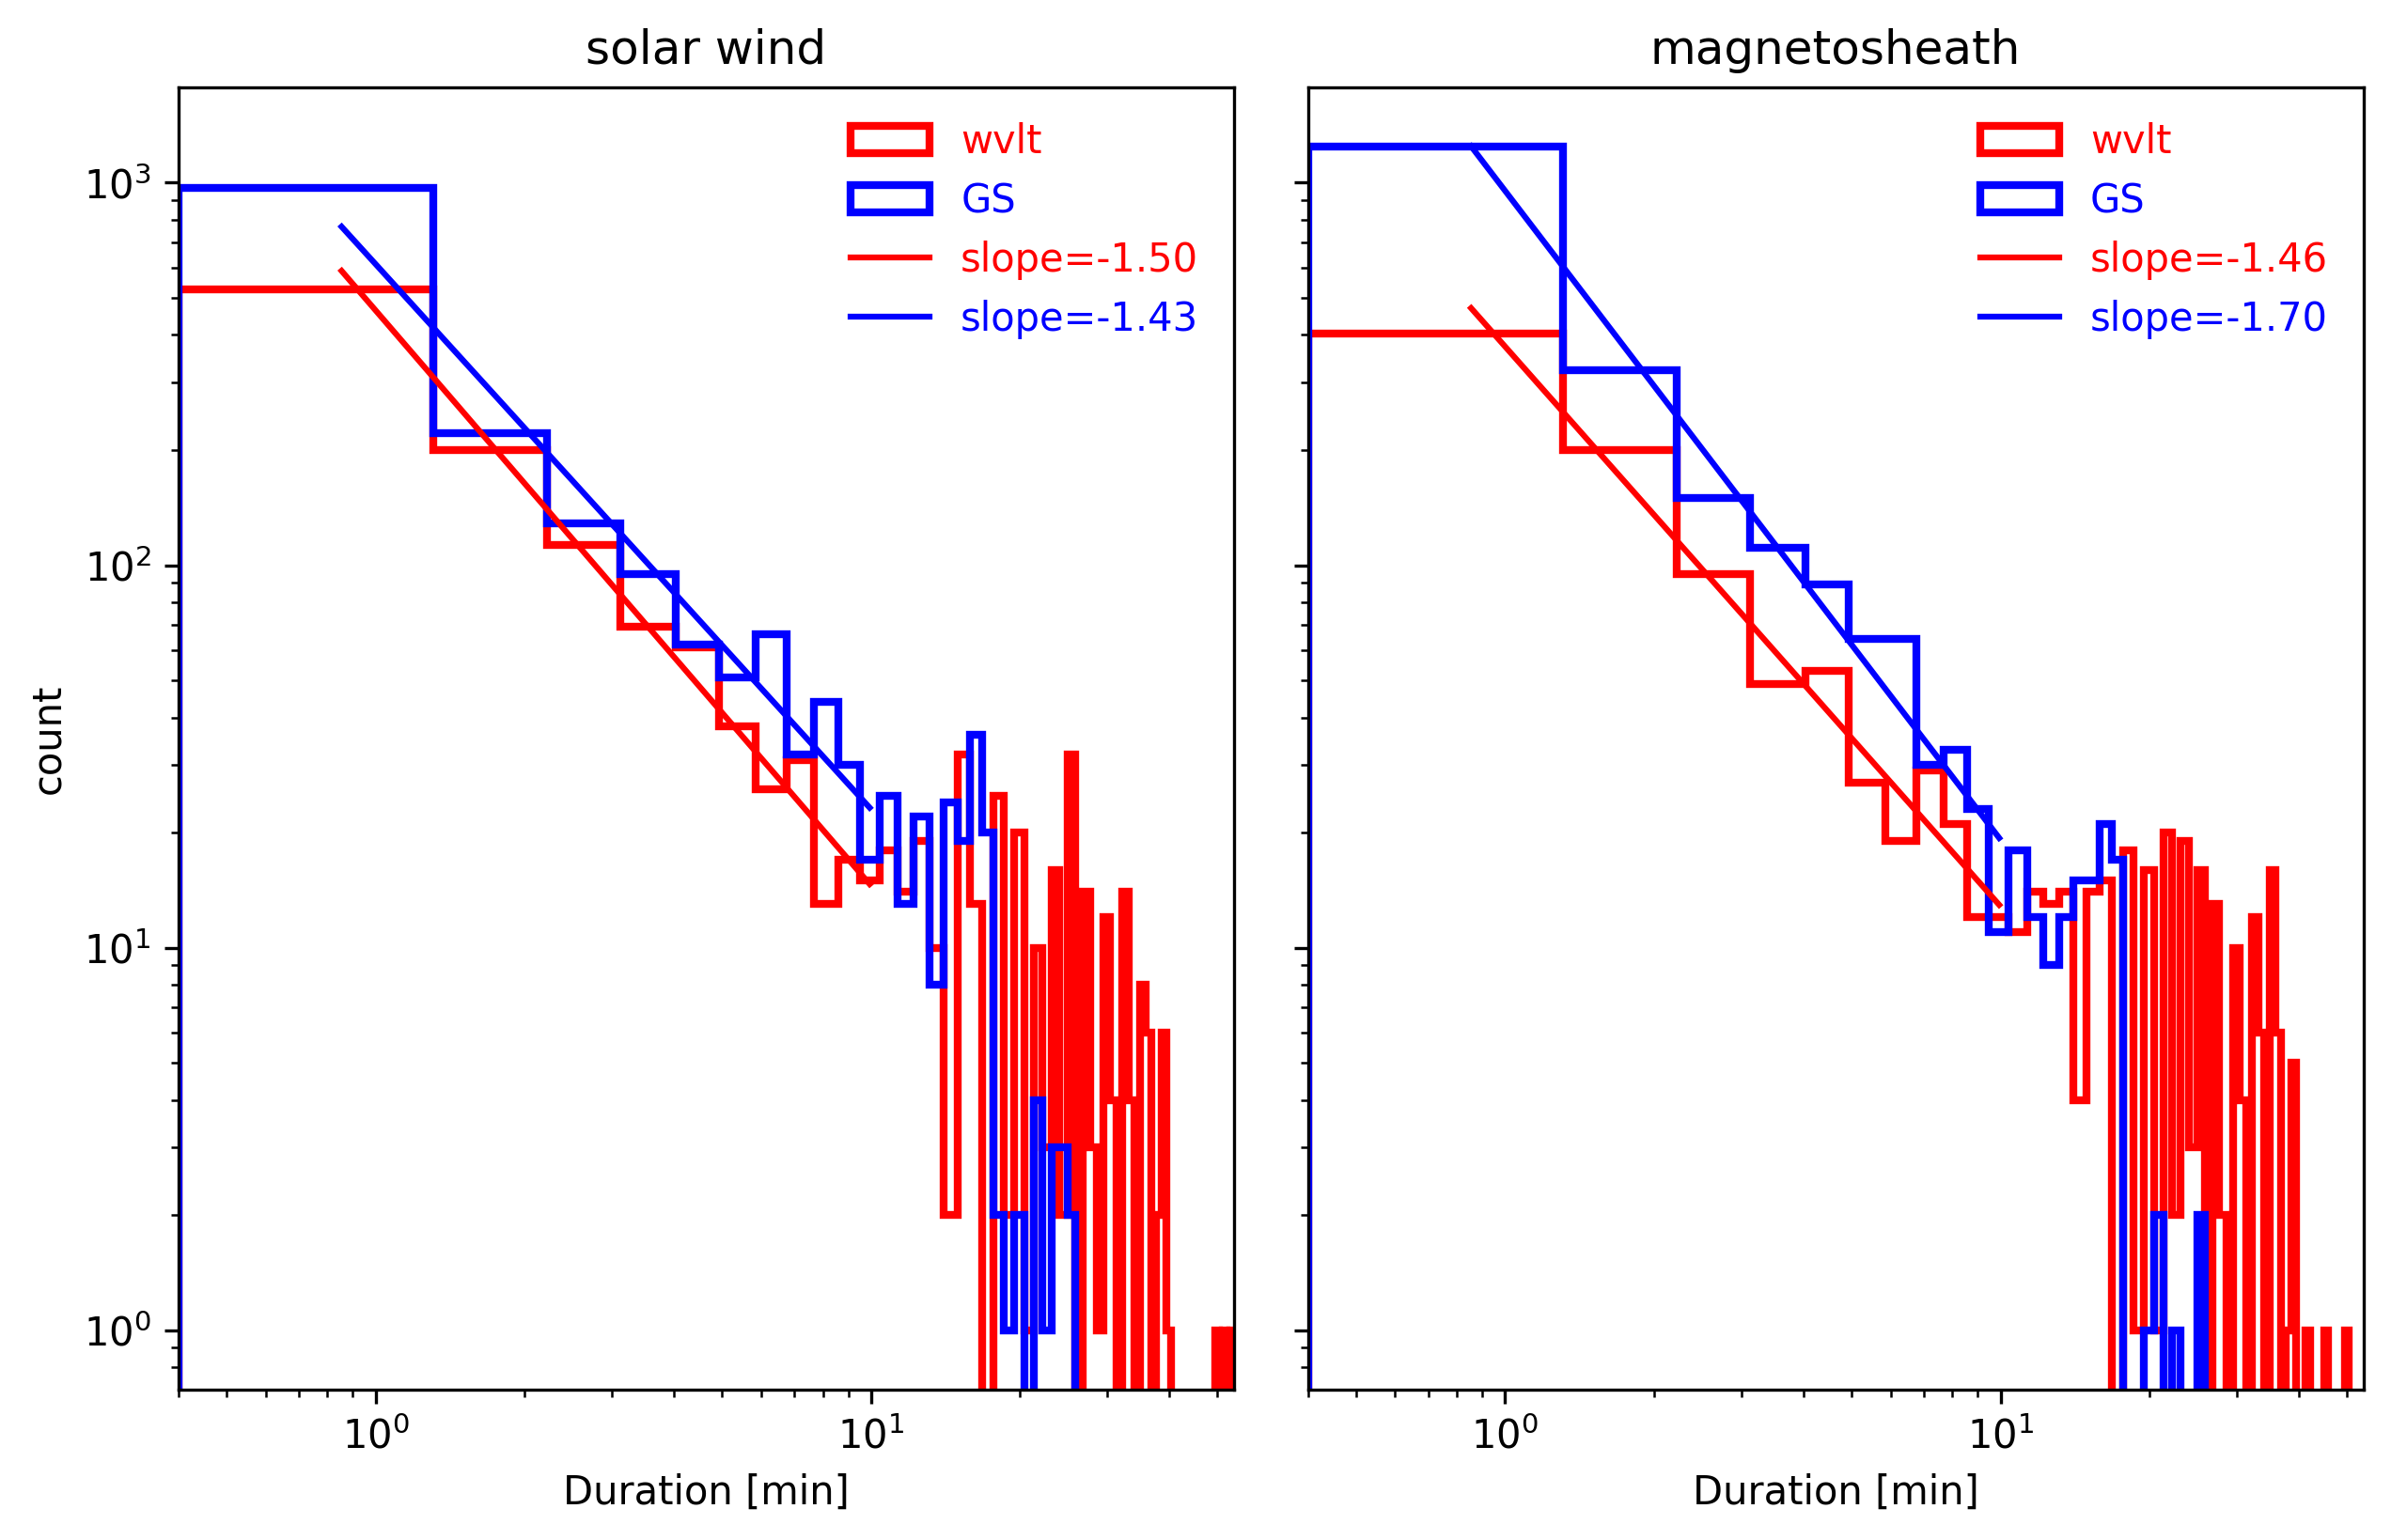
\includegraphics[width=\textwidth]{Figures/Histograms/duration_coordinated.png}
    \caption[Histogram of duration from coordinated analysis]{Histogram of the duration of events identified (during the coordinated orbit intervals) by using wavelet analysis (red lines) and the GS reconstruction method (blue lines).}
    \label{fig:histogram-duration-coordinated}
\end{figure}

\begin{figure}
    \centering
    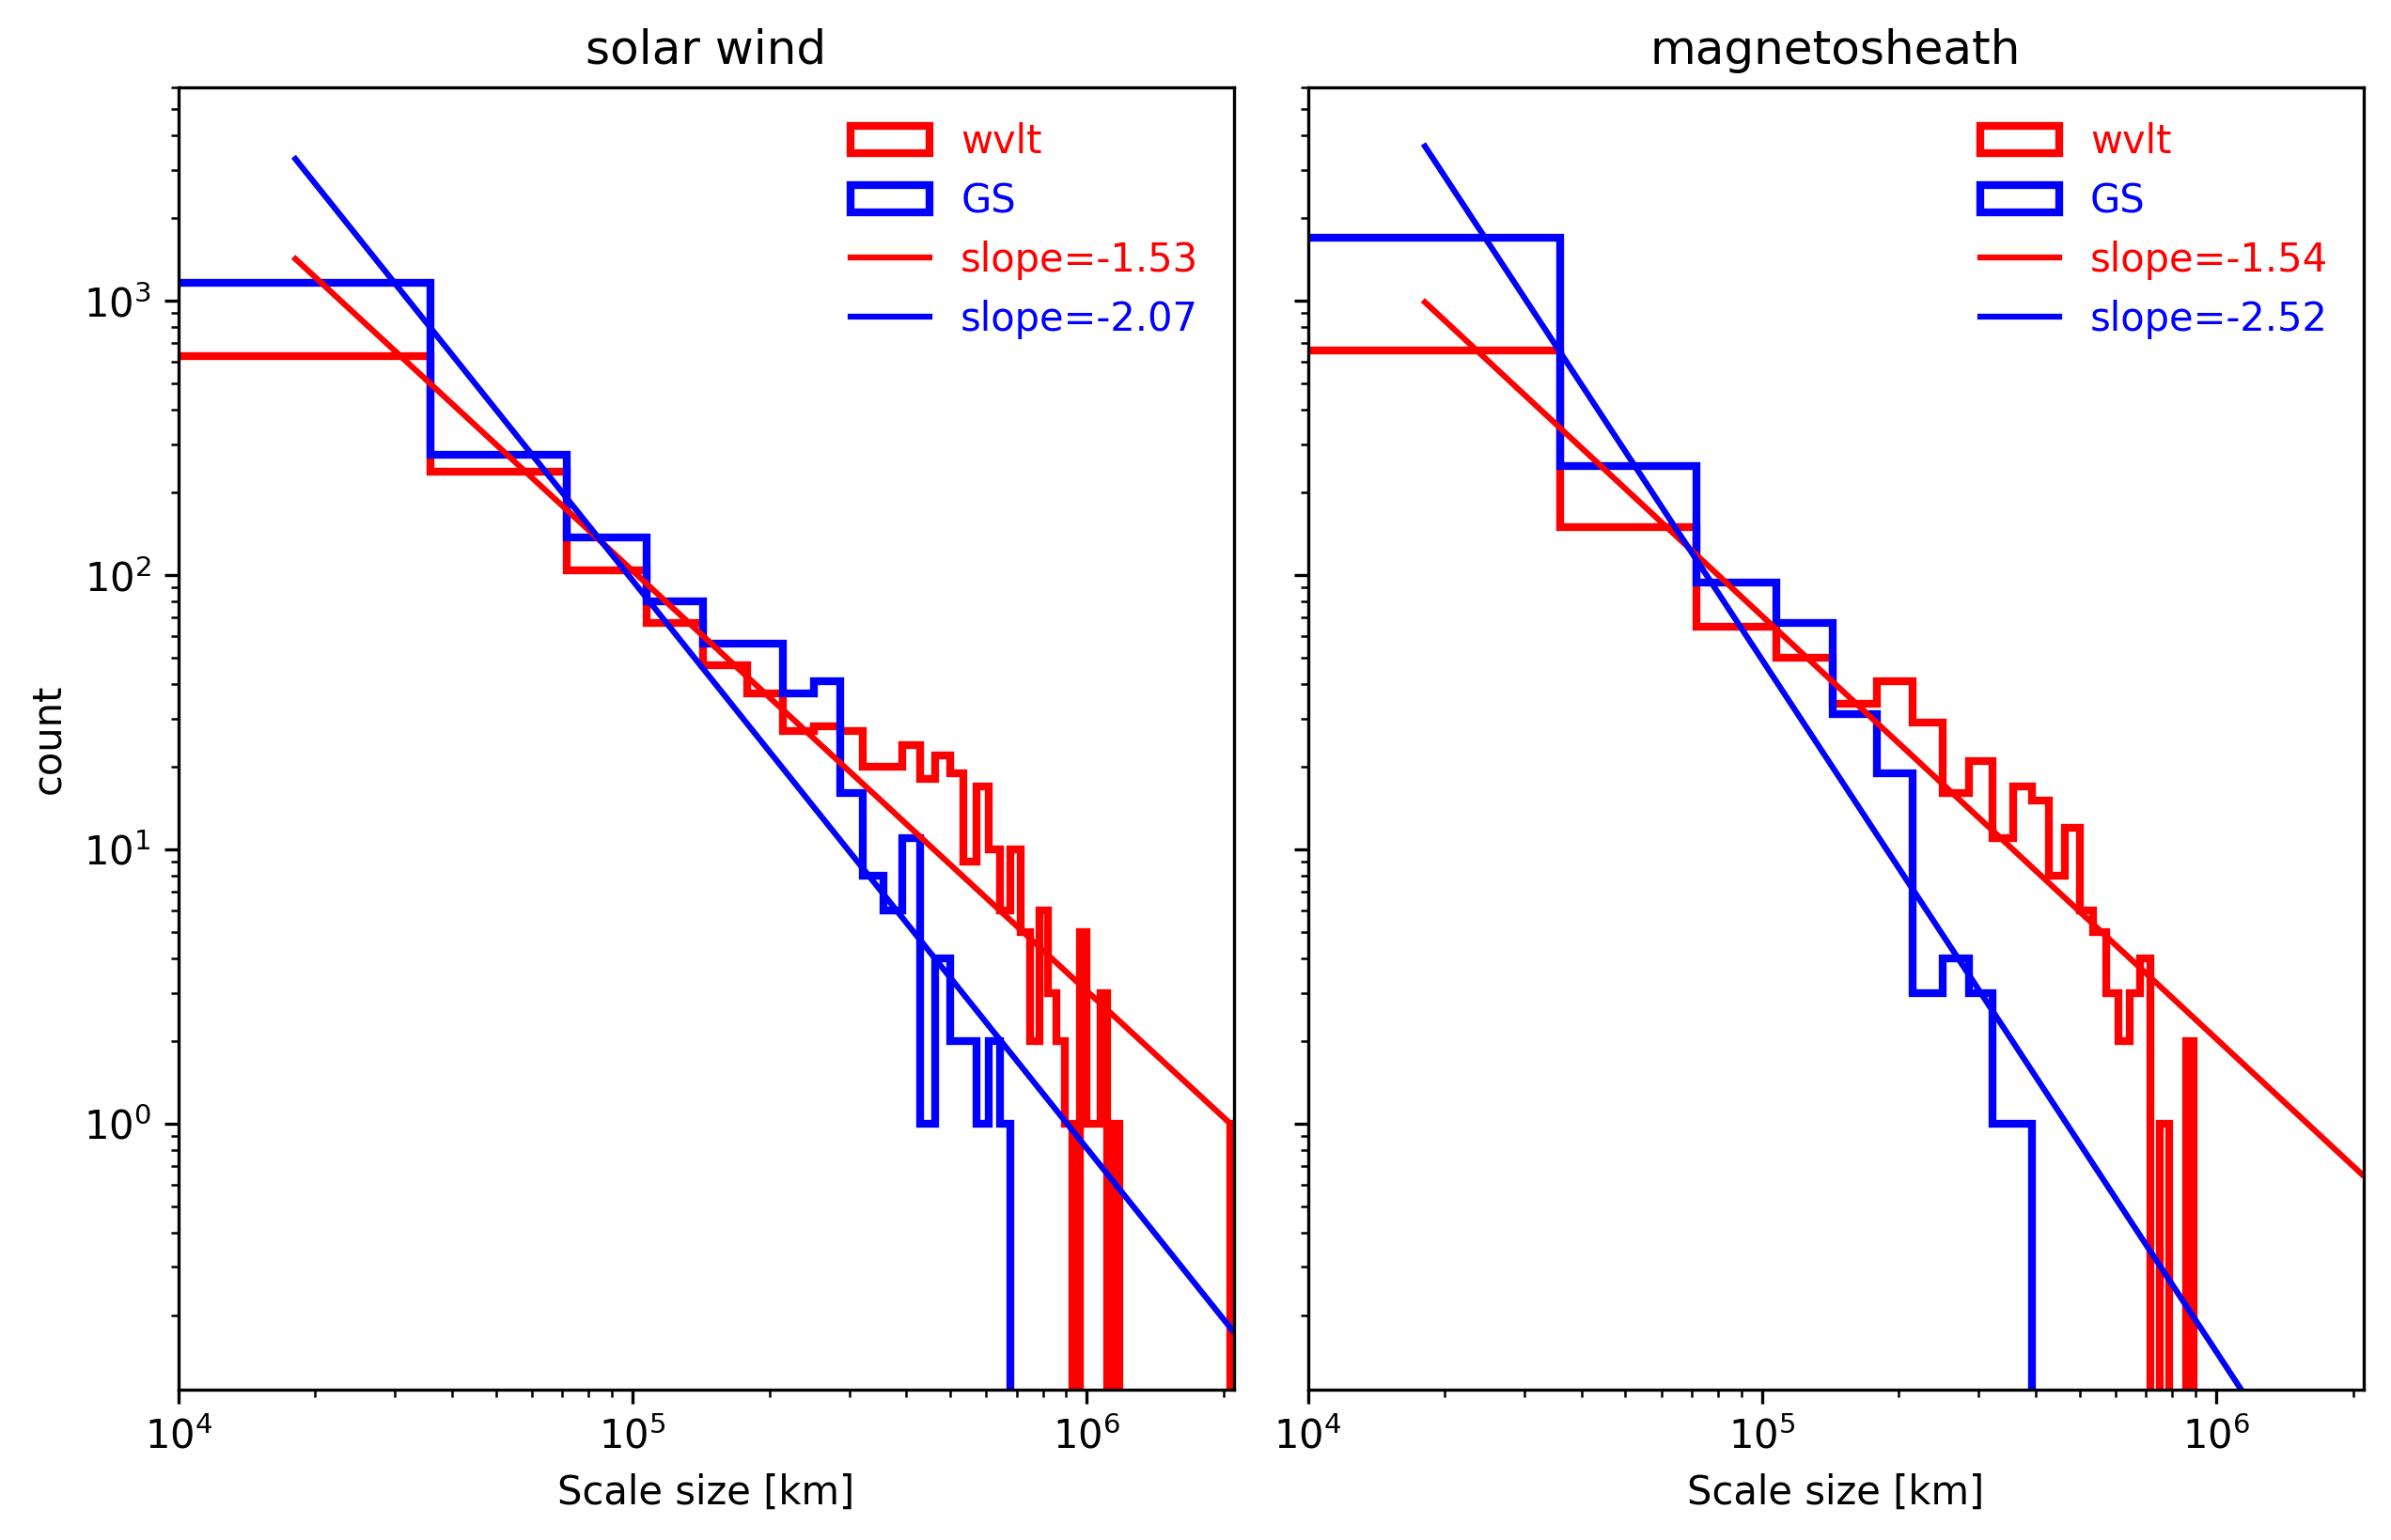
\includegraphics[width=\textwidth]{Figures/Histograms/scalesize_coordinated.png}
    \caption[Histogram of scale size from coordinated analysis]{Same as Figure \ref{fig:histogram-duration-coordinated} but for scale size of events identified during the coordinated orbit intervals.}
    \label{fig:histogram-scalesize-coordinated}
\end{figure}

\begin{figure}
    \centering
    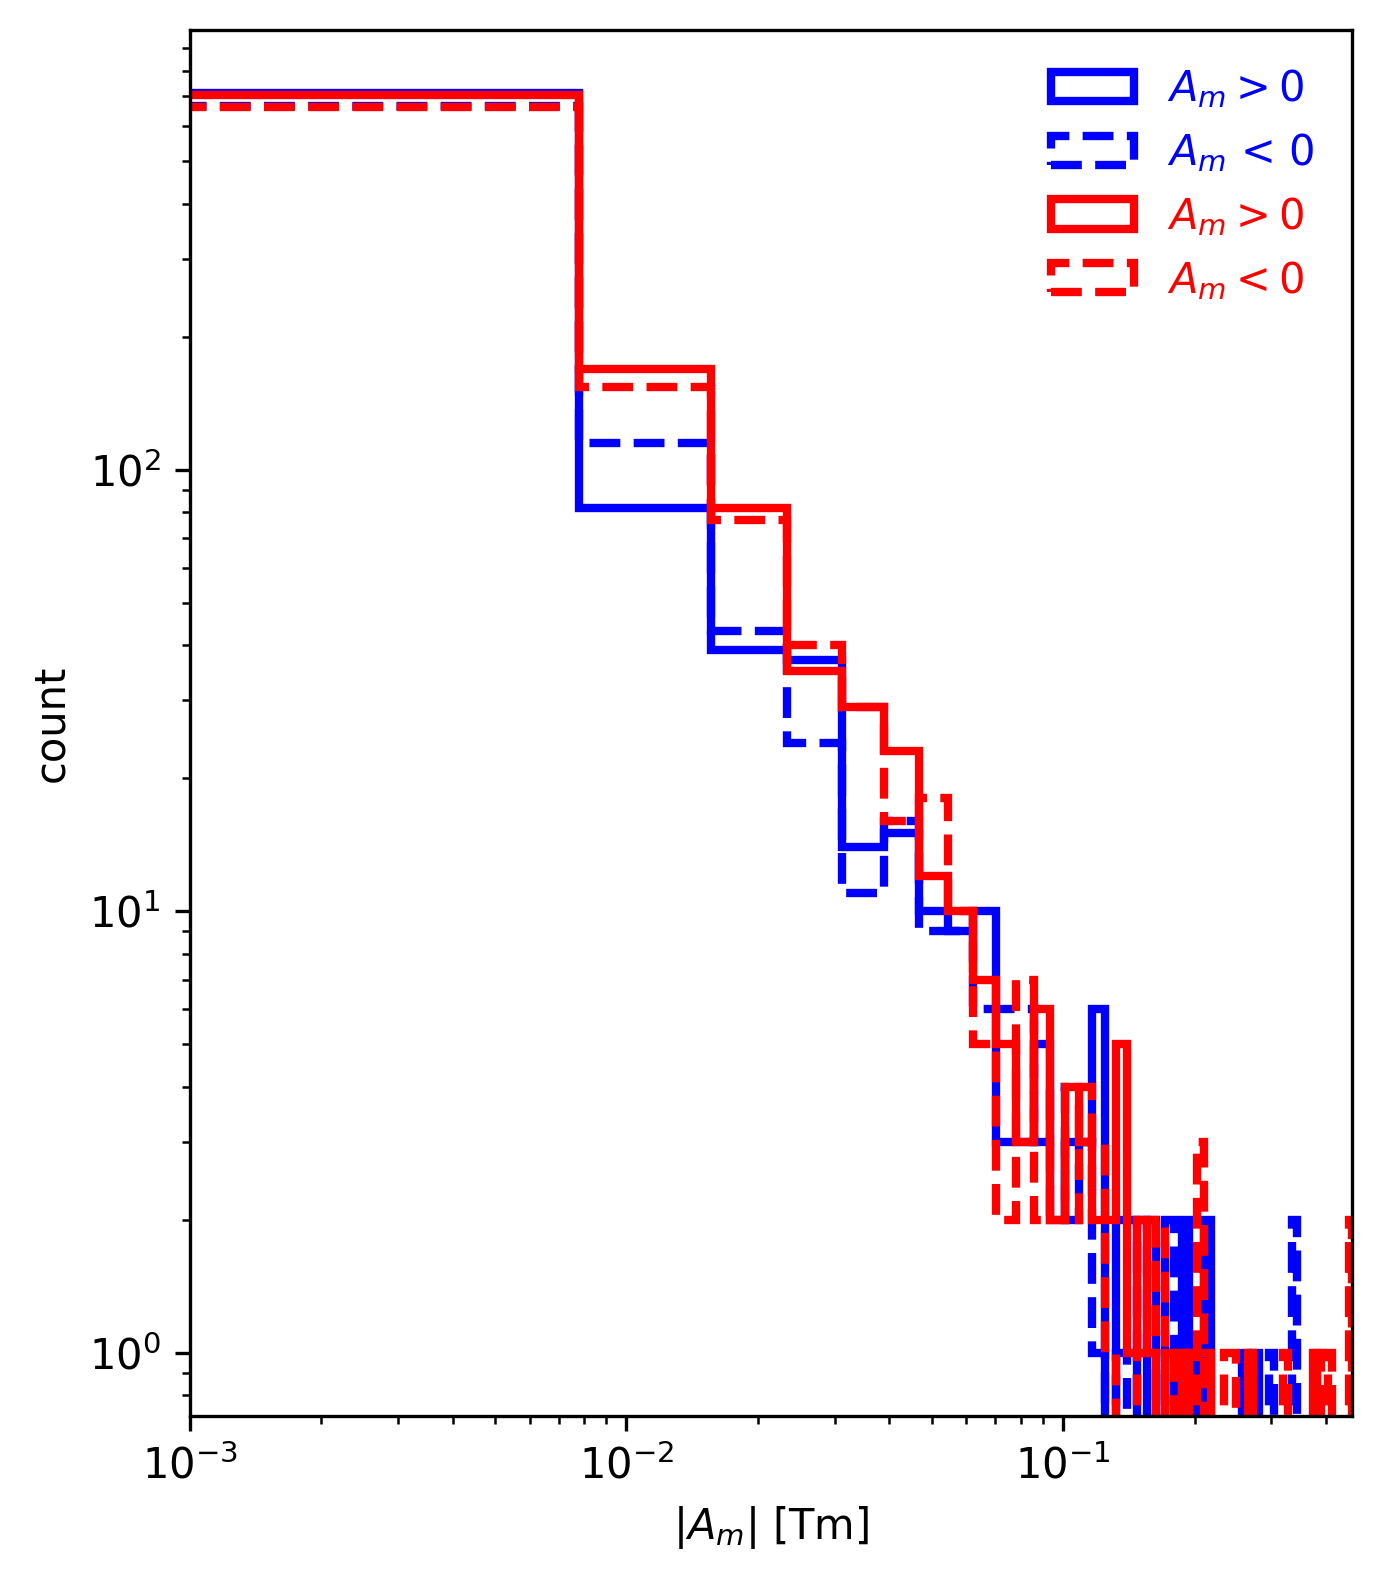
\includegraphics[width=0.7\textwidth]{Figures/Histograms/Asplit_coordinated.png}
    \caption[Histogram of poloidal magnetic flux per unit length from coordinated analysis]{Histograms for the local maximum magnetic flux $|A_m|$ of events identified via GS analysis during the coordinated orbit intervals.} %poloidal magnetic flux per unit length
    \label{fig:histogram-Asplit-coordinated}
\end{figure}



\begin{figure}
    \centering
    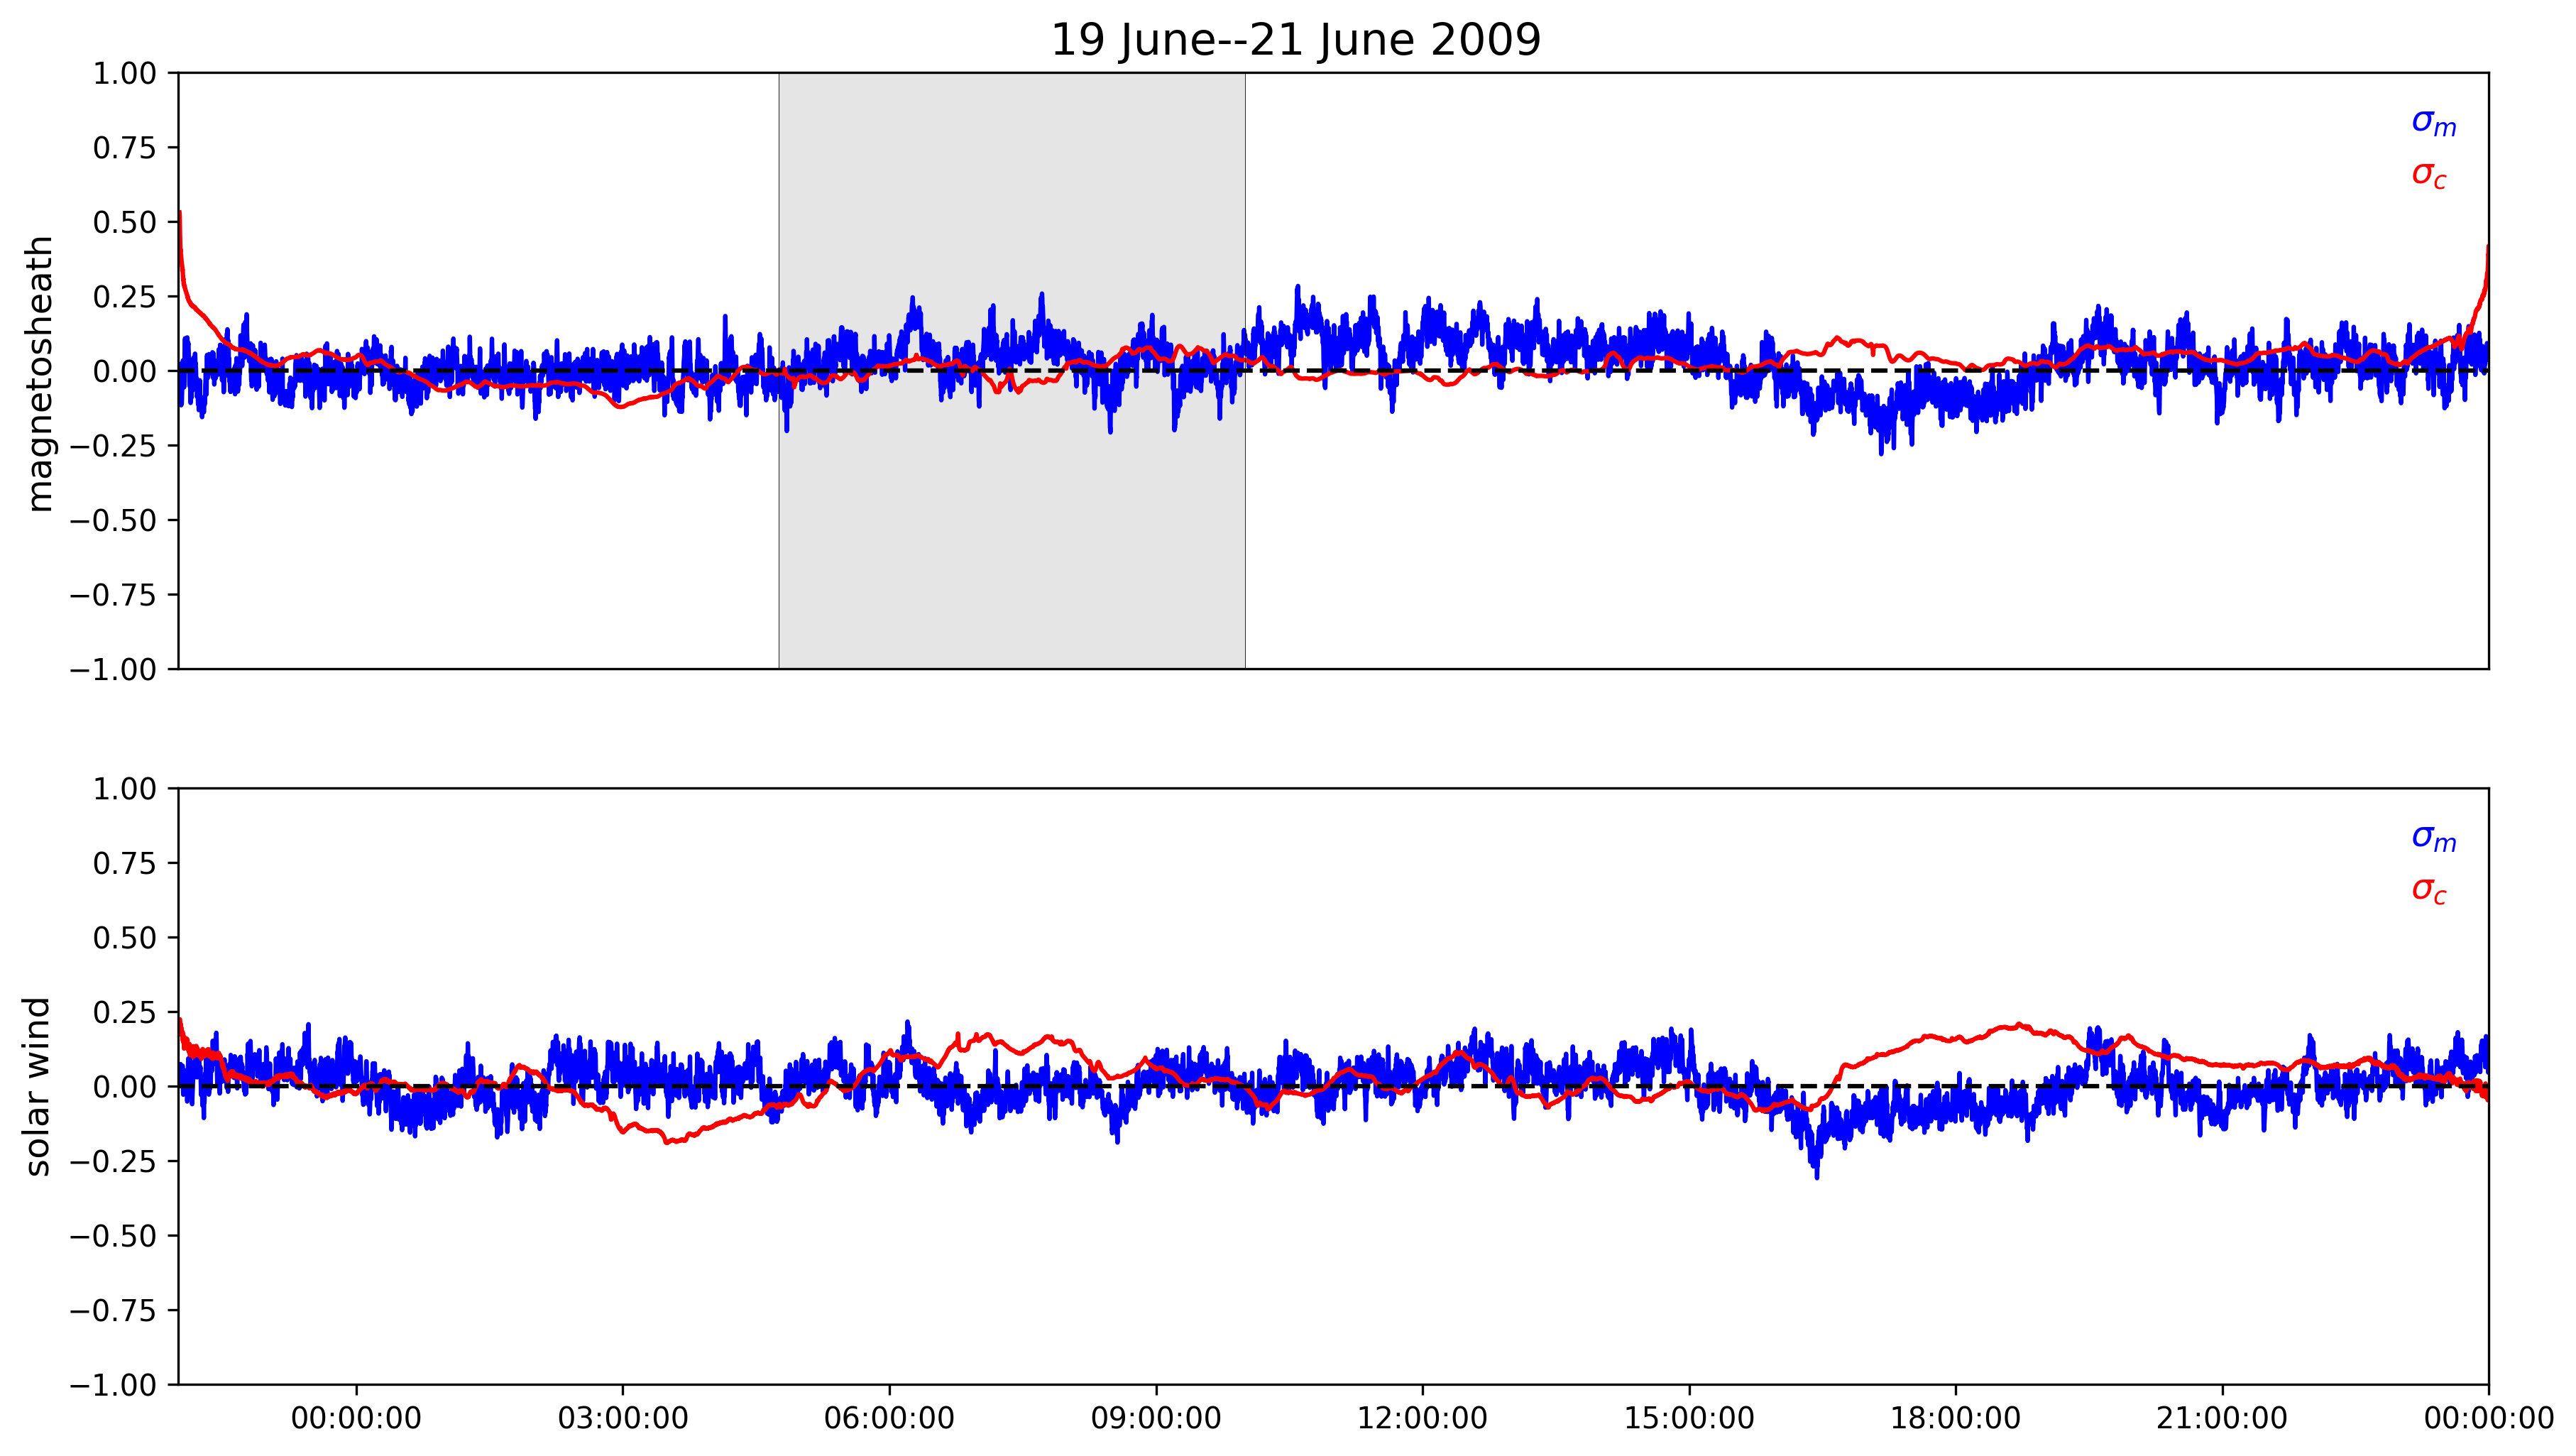
\includegraphics[width=\linewidth]{Figures/sigm_sigc_coordinated_20090619_20090621.png}
    \caption[Average reduced magnetic helicity and reduced cross helicity over time for 19-21 June 2009]{The average reduced magnetic helicity $\sigma_m$ and reduced cross helicity $\sigma_c$ as calculated by the wavelet analysis method (equations \ref{eq:sigm} and \ref{eq:sigc}) over one observation period by THM-C in the magnetosheath and THM-B in the solar wind over 19-21 June 2009. The grey interval in the top panel represents a bow shock crossing that is not included in our study.}
    \label{fig:mhd-over-time}
\end{figure}

%************************
%Back Matter of your Thesis Begins
%************************
\backmatter

%***********************
%References
%***********************
\addcontentsline{toc}{chapter}{References} %This adds the Bibliography/References to your table of contents.
\bibliographystyle{apalike} %This selects your bibliography style. There are many possible bibliography styles you can choose. The following site explains the options. https://www.overleaf.com/learn/latex/Bibtex_bibliography_styles


\begingroup %Begins an editable environment to set proper spacing for the bibliography/references page.
\setlength{\bibsep}{12pt} %This provides 10 pts between reference entries.
\setstretch{1} %This specifies single-spacing within entries.
\bibliography{references} %This inserts your References. You must individually add all references to the ref.bib file. Then, only those references you actually cite in the body of your text will be included.
\endgroup

%***********************
%Appendix Section: Optional. If you do not want to include any appendices, simply delete the below commands that create the appendix environment and that input your appendix file(s).
%**********************
\appendix %This creates the appendix environment. 

% Be sure to include the Heading Appendix A: before you type the name of the Appendix.
\chapter{Appendix A: Summary of observation intervals}\label{appendix:observation-periods}
% Appendices should appear at the very end of your thesis. Make sure to label each Appendix with a letter starting with "A". Any tables and/or figures located in the appendix should be labeled accordingly. For example, below is figure A.1 because it is the first figure that appears in Appendix A.

%If you add another appendix, copy and paste this line, but update it to B instead of A.
\renewcommand{\thechapter}{A}
\setcounter{table}{0}
\renewcommand{\thetable}{A.\arabic{table}}

% Magnetosheath
\begin{landscape}
\begin{spacing}{.5}
    \begin{longtable}{r|cccccccc}
\caption{Periods of data across 1051 hours in the magnetosheath from THEMIS and MMS probes} \\
\hline
{} &                     Start &                       End &  Probe &  \# Hours & Events \\
\hline
13 May 2008    &  2008-05-13 00:04:18.0946 &  2008-05-13 05:24:58.1467 &  THM-C &    5.344 &     86 \\
16-17 May 2008 &  2008-05-16 20:00:40.8048 &  2008-05-17 06:27:58.8540 &  THM-C &   10.455 &    210 \\
22 May 2008    &  2008-05-22 12:02:32.3340 &  2008-05-22 21:59:55.6656 &  THM-C &    9.956 &    159 \\
28-29 May 2008 &  2008-05-28 12:05:27.8539 &  2008-05-29 05:59:58.7792 &  THM-C &   17.908 &    246 \\
1-2 Jun 2008   &  2008-06-01 08:03:03.5541 &  2008-06-02 03:59:58.6605 &  THM-C &   19.949 &    260 \\
31 May 2009    &  2009-05-31 02:04:31.7145 &  2009-05-31 16:12:58.5210 &  THM-C &   14.141 &    295 \\
4 Jun 2009     &  2009-06-04 02:03:56.0925 &  2009-06-04 20:46:58.0740 &  THM-C &   18.717 &    233 \\
8 Jun 2009     &  2009-06-08 02:01:11.6000 &  2009-06-08 21:59:58.1120 &  THM-C &   19.979 &    396 \\
10 Jun 2009    &  2009-06-10 02:00:06.7896 &  2009-06-10 15:59:57.9210 &  THM-C &   13.998 &    190 \\
12 Jun 2009    &  2009-06-12 00:06:08.0568 &  2009-06-12 23:59:58.3656 &  THM-C &   23.897 &    304 \\
14 Jun 2009    &  2009-06-14 00:02:43.2510 &  2009-06-14 17:59:58.7742 &  THM-C &   17.954 &    140 \\
16 Jun 2009    &  2009-06-16 00:07:40.0400 &  2009-06-16 23:59:58.4800 &  THM-C &   23.872 &    184 \\
19-20 Jun 2009 &  2009-06-19 22:00:39.0672 &  2009-06-20 23:59:56.7312 &  THM-C &   25.988 &    233 \\
8 Sep 2015     &  2015-09-08 10:43:03.0000 &  2015-09-08 17:59:55.5000 &  MMS-1 &    7.281 &     97 \\
1 Oct 2015     &  2015-10-01 06:53:01.5000 &  2015-10-01 17:23:55.5000 &  MMS-1 &   10.515 &     79 \\
7 Oct 2015     &  2015-10-07 06:02:01.5000 &  2015-10-07 11:19:57.0000 &  MMS-1 &    5.299 &     53 \\
12 Oct 2015    &  2015-10-12 06:21:58.5000 &  2015-10-12 17:12:58.5000 &  MMS-1 &   10.850 &     68 \\
13 Oct 2015    &  2015-10-13 05:39:00.0000 &  2015-10-13 11:09:58.5000 &  MMS-1 &    5.516 &     91 \\
15 Oct 2015    &  2015-10-15 06:48:00.0000 &  2015-10-15 13:30:58.5000 &  MMS-1 &    6.716 &     60 \\
17 Oct 2015    &  2015-10-17 04:55:57.0000 &  2015-10-17 16:01:57.0000 &  MMS-1 &   11.100 &     83 \\
18 Oct 2015    &  2015-10-18 04:49:25.5000 &  2015-10-18 15:06:58.5000 &  MMS-1 &   10.293 &     69 \\
20 Oct 2015    &  2015-10-20 05:55:57.0000 &  2015-10-20 17:10:57.0000 &  MMS-1 &   11.250 &     99 \\
22 Oct 2015    &  2015-10-22 06:06:00.0000 &  2015-10-22 14:53:55.5000 &  MMS-1 &    8.799 &     83 \\
23 Oct 2015    &  2015-10-23 08:21:00.0000 &  2015-10-23 15:39:58.5000 &  MMS-1 &    7.316 &     70 \\
29 Oct 2015    &  2015-10-29 04:39:58.5000 &  2015-10-29 14:59:55.5000 &  MMS-1 &   10.332 &     75 \\
30 Oct 2015    &  2015-10-30 05:15:58.5000 &  2015-10-30 16:04:57.0000 &  MMS-1 &   10.816 &     75 \\
31 Oct 2015    &  2015-10-31 07:17:01.5000 &  2015-10-31 15:53:55.5000 &  MMS-1 &    8.615 &     91 \\
1 Nov 2015     &  2015-11-01 03:24:00.0000 &  2015-11-01 15:06:58.5000 &  MMS-1 &   11.716 &    119 \\
2 Nov 2015     &  2015-11-02 04:00:00.0000 &  2015-11-02 11:59:55.5000 &  MMS-1 &    7.999 &     57 \\
4 Nov 2015     &  2015-11-04 08:06:00.0000 &  2015-11-04 15:30:58.5000 &  MMS-1 &    7.416 &     59 \\
5 Nov 2015     &  2015-11-05 07:06:00.0000 &  2015-11-05 14:21:58.5000 &  MMS-1 &    7.266 &     72 \\
10 Nov 2015    &  2015-11-10 02:48:58.5000 &  2015-11-10 08:36:58.5000 &  MMS-1 &    5.800 &     60 \\
13 Nov 2015    &  2015-11-13 04:54:00.0000 &  2015-11-13 10:21:58.5000 &  MMS-1 &    5.466 &     60 \\
14 Nov 2015    &  2015-11-14 03:13:57.0000 &  2015-11-14 12:35:55.5000 &  MMS-1 &    9.366 &     74 \\
6 Dec 2015     &  2015-12-06 08:14:01.5000 &  2015-12-06 13:30:58.5000 &  MMS-1 &    5.282 &    157 \\
25 Oct 2016    &  2016-10-25 09:44:28.5000 &  2016-10-25 18:24:58.5000 &  MMS-1 &    8.675 &     79 \\
3 Nov 2016     &  2016-11-03 08:39:18.0000 &  2016-11-03 15:03:58.5000 &  MMS-1 &    6.411 &     96 \\
8 Nov 2016     &  2016-11-08 09:35:01.5000 &  2016-11-08 14:39:58.5000 &  MMS-1 &    5.082 &     58 \\
10 Nov 2016    &  2016-11-10 08:16:57.0000 &  2016-11-10 16:59:55.5000 &  MMS-1 &    8.716 &     71 \\
11 Nov 2016    &  2016-11-11 09:11:01.5000 &  2016-11-11 18:27:58.5000 &  MMS-1 &    9.283 &     69 \\
12 Nov 2016    &  2016-11-12 07:42:58.5000 &  2016-11-12 17:48:58.5000 &  MMS-1 &   10.100 &     89 \\
19 Nov 2016    &  2016-11-19 08:00:00.0000 &  2016-11-19 17:50:55.5000 &  MMS-1 &    9.849 &     62 \\
20 Nov 2016    &  2016-11-20 11:27:58.5000 &  2016-11-20 17:20:55.5000 &  MMS-1 &    5.883 &     51 \\
21 Nov 2016    &  2016-11-21 11:56:01.5000 &  2016-11-21 19:20:55.5000 &  MMS-1 &    7.415 &     74 \\
22 Nov 2016    &  2016-11-22 06:43:57.0000 &  2016-11-22 18:20:55.5000 &  MMS-1 &   11.616 &     85 \\
23 Nov 2016    &  2016-11-23 10:33:00.0000 &  2016-11-23 16:47:55.5000 &  MMS-1 &    6.249 &     71 \\
24 Nov 2016    &  2016-11-24 06:14:10.5000 &  2016-11-24 18:35:55.5000 &  MMS-1 &   12.363 &     88 \\
27 Nov 2016    &  2016-11-27 06:58:03.0000 &  2016-11-27 12:47:55.5000 &  MMS-1 &    5.831 &     61 \\
1 Dec 2016     &  2016-12-01 06:32:01.5000 &  2016-12-01 16:53:55.5000 &  MMS-1 &   10.365 &     65 \\
3 Dec 2016     &  2016-12-03 07:15:00.0000 &  2016-12-03 16:14:55.5000 &  MMS-1 &    8.999 &    106 \\
4 Dec 2016     &  2016-12-04 06:15:59.0013 &  2016-12-04 17:35:56.9079 &  MMS-1 &   11.332 &    111 \\
5 Dec 2016     &  2016-12-05 04:54:22.5000 &  2016-12-05 12:47:55.5000 &  MMS-1 &    7.893 &     68 \\
7 Dec 2016     &  2016-12-07 05:12:58.5000 &  2016-12-07 14:36:58.5000 &  MMS-1 &    9.400 &     79 \\
8 Dec 2016     &  2016-12-08 10:03:58.5000 &  2016-12-08 15:58:57.0000 &  MMS-1 &    5.916 &     65 \\
9 Dec 2016     &  2016-12-09 11:48:58.5000 &  2016-12-09 17:56:55.5000 &  MMS-1 &    6.133 &     37 \\
11 Dec 2016    &  2016-12-11 09:46:57.0000 &  2016-12-11 15:42:58.5000 &  MMS-1 &    5.934 &     40 \\
18 Dec 2016    &  2016-12-18 07:51:00.0000 &  2016-12-18 14:36:58.5000 &  MMS-1 &    6.766 &     74 \\
24 Dec 2016    &  2016-12-24 07:36:00.0000 &  2016-12-24 14:51:58.5000 &  MMS-1 &    7.266 &     59 \\
3 Oct 2017     &  2017-10-03 12:00:00.0000 &  2017-10-03 18:59:55.5000 &  MMS-1 &    6.999 &    188 \\
6 Oct 2017     &  2017-10-06 14:10:07.5000 &  2017-10-06 17:59:55.5000 &  MMS-1 &    3.830 &    720 \\
5 Nov 2017     &  2017-11-05 03:30:00.0000 &  2017-11-05 11:59:55.5000 &  MMS-1 &    8.499 &    113 \\
8 Nov 2017     &  2017-11-08 01:30:00.0000 &  2017-11-08 05:59:55.5000 &  MMS-1 &    4.499 &     56 \\
14 Nov 2017    &  2017-11-14 15:00:00.0000 &  2017-11-14 19:57:58.5000 &  MMS-1 &    4.966 &     36 \\
22 Nov 2017    &  2017-11-22 05:38:01.5000 &  2017-11-22 10:55:57.0000 &  MMS-1 &    5.299 &     58 \\
25 Nov 2017    &  2017-11-25 01:26:01.5000 &  2017-11-25 07:09:58.5000 &  MMS-1 &    5.732 &     67 \\
30 Nov 2017    &  2017-11-30 16:23:01.5000 &  2017-11-30 23:01:57.0000 &  MMS-1 &    6.649 &     57 \\
3 Dec 2017     &  2017-12-03 11:16:30.0000 &  2017-12-03 18:47:55.5000 &  MMS-1 &    7.524 &     80 \\
9 Dec 2017     &  2017-12-09 03:15:27.0000 &  2017-12-09 08:28:57.0000 &  MMS-1 &    5.225 &     55 \\
13 Sep 2018    &  2018-09-13 17:02:03.1612 &  2018-09-13 21:59:55.9729 &  THM-E &    4.964 &     51 \\
14-15 Sep 2018 &  2018-09-14 14:00:01.5774 &  2018-09-15 03:52:27.7438 &  THM-E &   13.874 &     86 \\
21 Oct 2018    &  2018-10-21 10:00:58.5000 &  2018-10-21 19:23:55.5000 &  MMS-1 &    9.383 &     83 \\
24 Oct 2018    &  2018-10-24 07:59:01.5000 &  2018-10-24 16:01:57.0000 &  MMS-1 &    8.049 &     74 \\
27 Oct 2018    &  2018-10-27 04:19:57.0000 &  2018-10-27 23:56:55.5000 &  MMS-1 &   19.616 &    166 \\
30 Oct 2018    &  2018-10-30 00:24:00.0000 &  2018-10-30 05:24:58.5000 &  MMS-1 &    5.016 &     50 \\
1 Nov 2018     &  2018-11-01 16:53:01.5000 &  2018-11-01 23:59:55.5000 &  MMS-1 &    7.115 &     72 \\
4 Nov 2018     &  2018-11-04 11:50:01.5000 &  2018-11-04 17:29:55.5000 &  MMS-1 &    5.665 &     32 \\
10 Nov 2018    &  2018-11-10 16:35:01.5000 &  2018-11-10 23:57:58.5000 &  MMS-1 &    7.383 &     33 \\
13 Nov 2018    &  2018-11-13 12:24:00.0000 &  2018-11-13 19:29:55.5000 &  MMS-1 &    7.099 &     68 \\
14 Nov 2018    &  2018-11-14 17:42:58.5000 &  2018-11-14 23:06:58.5000 &  MMS-1 &    5.400 &     74 \\
17 Nov 2018    &  2018-11-17 12:23:01.5000 &  2018-11-17 19:36:58.5000 &  MMS-1 &    7.232 &     65 \\
21 Nov 2018    &  2018-11-21 08:48:58.5000 &  2018-11-21 17:17:55.5000 &  MMS-1 &    8.482 &     96 \\
23 Nov 2018    &  2018-11-23 09:15:00.0000 &  2018-11-23 15:03:58.5000 &  MMS-1 &    5.816 &     59 \\
26 Nov 2018    &  2018-11-26 00:29:01.5000 &  2018-11-26 09:08:55.5000 &  MMS-1 &    8.665 &     79 \\
29 Nov 2018    &  2018-11-29 00:09:00.0000 &  2018-11-29 06:06:58.5000 &  MMS-1 &    5.966 &     66 \\
21 Dec 2018    &  2018-12-21 13:57:00.0000 &  2018-12-21 19:10:57.0000 &  MMS-1 &    5.232 &     72 \\
26 Oct 2019    &  2019-10-26 06:39:00.0000 &  2019-10-26 12:27:58.5000 &  MMS-1 &    5.816 &     53 \\
2 Nov 2019     &  2019-11-02 08:48:00.0000 &  2019-11-02 18:04:57.0000 &  MMS-1 &    9.283 &    118 \\
6 Nov 2019     &  2019-11-06 11:36:00.0000 &  2019-11-06 23:26:55.5000 &  MMS-1 &   11.849 &     61 \\
9 Nov 2019     &  2019-11-09 08:50:01.5000 &  2019-11-09 15:17:55.5000 &  MMS-1 &    6.465 &     82 \\
13 Nov 2019    &  2019-11-13 00:00:04.5000 &  2019-11-13 07:52:57.0000 &  MMS-1 &    7.881 &     53 \\
19 Nov 2019    &  2019-11-19 18:15:00.0000 &  2019-11-19 23:59:55.5000 &  MMS-1 &    5.749 &     47 \\
23 Nov 2019    &  2019-11-23 07:32:01.5000 &  2019-11-23 13:23:55.5000 &  MMS-1 &    5.865 &     50 \\
6 Dec 2019     &  2019-12-06 07:05:01.5000 &  2019-12-06 16:02:55.5000 &  MMS-1 &    8.965 &    123 \\
10 Dec 2019    &  2019-12-10 00:00:04.5000 &  2019-12-10 05:25:57.0000 &  MMS-1 &    5.431 &     72 \\
13 Dec 2019    &  2019-12-13 09:42:58.5000 &  2019-12-13 15:18:58.5000 &  MMS-1 &    5.600 &     54 \\
17 Dec 2019    &  2019-12-17 00:00:04.5000 &  2019-12-17 03:59:55.5000 &  MMS-1 &    3.998 &     63 \\
24 Dec 2019    &  2019-12-24 00:00:04.5000 &  2019-12-24 05:44:55.5000 &  MMS-1 &    5.747 &     46 \\
31 Oct 2020    &  2020-10-31 10:47:01.5000 &  2020-10-31 15:04:57.0000 &  MMS-1 &    4.299 &     38 \\
14 Nov 2020    &  2020-11-14 08:37:03.0000 &  2020-11-14 17:21:58.5000 &  MMS-1 &    8.749 &     80 \\
2 Dec 2020     &  2020-12-02 00:00:04.5000 &  2020-12-02 08:59:55.5000 &  MMS-1 &    8.998 &     63 \\
7 Dec 2020     &  2020-12-07 16:30:00.0000 &  2020-12-07 23:59:55.5000 &  MMS-1 &    7.499 &     63 \\
11 Dec 2020    &  2020-12-11 07:12:00.0000 &  2020-12-11 14:09:58.5000 &  MMS-1 &    6.966 &     73 \\
7 Nov 2021     &  2021-11-07 04:12:00.0000 &  2021-11-07 14:05:55.5000 &  MMS-1 &    9.899 &    157 \\
14 Nov 2021    &  2021-11-14 03:30:00.0000 &  2021-11-14 10:24:58.5000 &  MMS-1 &    6.916 &     47 \\
28 Nov 2021    &  2021-11-28 12:17:02.4827 &  2021-11-28 19:15:55.5412 &  MMS-1 &    6.981 &     54 \\
1 Dec 2021     &  2021-12-01 16:48:58.5000 &  2021-12-01 22:19:57.0000 &  MMS-1 &    5.516 &     64 \\
18 Dec 2021    &  2021-12-18 06:48:58.5000 &  2021-12-18 14:42:58.5000 &  MMS-1 &    7.900 &     88 \\
22 Dec 2021    &  2021-12-22 18:36:58.5000 &  2021-12-22 23:59:55.5000 &  MMS-1 &    5.383 &     48 \\
1 Jan 2022     &  2022-01-01 04:02:01.5000 &  2022-01-01 17:37:57.0000 &  MMS-1 &   13.599 &    116 \\
5 Jan 2022     &  2022-01-05 00:00:04.5000 &  2022-01-05 05:59:55.5000 &  MMS-1 &    5.997 &     59 \\
5 Jan 2022     &  2022-01-05 00:01:49.6800 &  2022-01-05 05:59:58.7340 &  THM-A &    5.969 &     43 \\
6 Jan 2022     &  2022-01-06 00:05:40.0080 &  2022-01-06 05:59:58.7340 &  THM-A &    5.905 &     91 \\
7 Jan 2022     &  2022-01-07 06:05:33.2580 &  2022-01-07 11:59:57.4680 &  THM-A &    5.907 &     68 \\
12 Jan 2022    &  2022-01-12 03:15:00.0000 &  2022-01-12 07:59:55.5000 &  MMS-1 &    4.749 &     41 \\
8 Nov 2022     &  2022-11-08 00:00:04.5000 &  2022-11-08 07:51:58.5000 &  MMS-1 &    7.865 &     90 \\
11 Nov 2022    &  2022-11-11 11:30:00.0000 &  2022-11-11 19:46:57.0000 &  MMS-1 &    8.283 &     40 \\
18 Nov 2022    &  2022-11-18 10:44:01.5000 &  2022-11-18 16:59:55.5000 &  MMS-1 &    6.265 &     51 \\
22 Nov 2022    &  2022-11-22 01:15:00.0000 &  2022-11-22 05:24:58.5000 &  MMS-1 &    4.166 &     71 \\
25 Nov 2022    &  2022-11-25 09:45:58.5000 &  2022-11-25 17:54:58.5000 &  MMS-1 &    8.150 &     72 \\
2 Dec 2022     &  2022-12-02 12:48:00.0000 &  2022-12-02 18:16:57.0000 &  MMS-1 &    5.482 &     74 \\
13 Dec 2022    &  2022-12-13 08:30:00.0000 &  2022-12-13 13:40:57.0000 &  MMS-1 &    5.183 &     55 \\
15 Dec 2022    &  2022-12-15 08:07:57.0000 &  2022-12-15 20:17:55.5000 &  MMS-1 &   12.166 &     86 \\
20 Dec 2022    &  2022-12-20 07:12:58.5000 &  2022-12-20 16:43:57.0000 &  MMS-1 &    9.516 &     51 \\
22 Dec 2022    &  2022-12-22 15:01:57.0000 &  2022-12-22 21:29:55.5000 &  MMS-1 &    6.466 &     46 \\
27 Dec 2022    &  2022-12-27 00:00:04.5000 &  2022-12-27 06:00:58.5000 &  MMS-1 &    6.015 &     49 \\
29 Dec 2022    &  2022-12-29 18:06:01.4480 &  2022-12-29 23:59:57.4199 &  MMS-1 &    5.899 &     80 \\
2 Jan 2023     &  2023-01-02 02:48:00.0000 &  2023-01-02 09:40:57.0000 &  MMS-1 &    6.883 &     82 \\
5 Jan 2023     &  2023-01-05 16:25:03.0000 &  2023-01-05 22:54:58.5000 &  MMS-1 &    6.499 &     69 \\
6 Jan 2023     &  2023-01-06 12:24:00.0000 &  2023-01-06 19:54:58.5000 &  MMS-1 &    7.516 &     47 \\
9 Jan 2023     &  2023-01-09 04:19:03.0000 &  2023-01-09 10:59:55.5000 &  MMS-1 &    6.681 &     58 \\
23 Jan 2023    &  2023-01-23 08:10:03.6534 &  2023-01-23 12:19:57.9866 &  MMS-1 &    4.165 &     38 \\
\hline
\end{longtable}

    \label{tab:msh-observations}
\end{spacing}
\end{landscape}

% Solar wind
\begin{landscape}
\begin{spacing}{.5}
    \begin{longtable}{r|cccccccc}
\caption{Periods of data across 676 hours in the solar wind from THEMIS and MMS probes} \\
\hline
{} &                     Start &                       End &  Probe &  \# Hours & Events \\
\hline
13 May 2008    &  2008-05-13 00:05:12.0000 &  2008-05-13 11:59:57.0000 &  THM-B &   11.912 &    157 \\
16-17 May 2008 &  2008-05-16 20:00:39.0000 &  2008-05-17 09:59:57.0000 &  THM-B &   13.988 &    298 \\
22 May 2008    &  2008-05-22 12:02:31.4450 &  2008-05-22 21:59:56.6398 &  THM-B &    9.957 &    132 \\
28-29 May 2008 &  2008-05-28 18:02:26.1648 &  2008-05-29 05:59:57.5998 &  THM-B &   11.959 &    182 \\
1-2 Jun 2008   &  2008-06-01 08:01:30.9630 &  2008-06-02 03:59:57.3598 &  THM-B &   19.974 &    256 \\
31 May 2009    &  2009-05-31 02:01:56.8480 &  2009-05-31 20:59:57.5310 &  THM-B &   18.967 &    295 \\
4 Jun 2009     &  2009-06-04 02:01:24.1835 &  2009-06-04 22:59:58.5685 &  THM-B &   20.976 &    220 \\
8 Jun 2009     &  2009-06-08 02:02:19.8640 &  2009-06-08 21:59:58.1120 &  THM-B &   19.961 &    262 \\
10 Jun 2009    &  2009-06-10 02:02:57.7022 &  2009-06-10 15:59:57.1216 &  THM-B &   13.950 &    155 \\
12 Jun 2009    &  2009-06-12 00:06:05.0271 &  2009-06-12 23:59:58.6501 &  THM-B &   23.898 &    309 \\
14 Jun 2009    &  2009-06-14 00:05:05.6731 &  2009-06-14 17:59:59.7295 &  THM-B &   17.915 &    140 \\
16 Jun 2009    &  2009-06-16 00:06:11.0000 &  2009-06-16 23:59:58.4800 &  THM-B &   23.896 &    280 \\
19-20 Jun 2009 &  2009-06-19 22:00:46.1956 &  2009-06-20 23:59:57.1872 &  THM-B &   25.986 &    269 \\
24 Oct 2017    &  2017-10-24 08:14:01.5000 &  2017-10-24 13:42:58.5000 &  MMS-1 &    5.482 &     57 \\
1 Nov 2017     &  2017-11-01 03:24:58.5000 &  2017-11-01 22:32:55.5000 &  MMS-1 &   19.133 &    111 \\
7 Nov 2017     &  2017-11-07 00:00:00.0000 &  2017-11-07 10:24:58.5000 &  MMS-1 &   10.416 &     63 \\
4 Dec 2017     &  2017-12-04 09:27:00.0000 &  2017-12-04 14:43:57.0000 &  MMS-1 &    5.282 &     51 \\
22 Dec 2017    &  2017-12-22 05:40:25.5000 &  2017-12-22 10:45:58.5000 &  MMS-1 &    5.093 &     35 \\
30 Dec 2017    &  2017-12-30 13:24:22.5000 &  2017-12-30 19:01:57.0000 &  MMS-1 &    5.626 &     50 \\
2 Jan 2018     &  2018-01-02 08:30:27.0000 &  2018-01-02 14:14:55.5000 &  MMS-1 &    5.741 &     77 \\
8 Jan 2018     &  2018-01-08 03:23:28.5000 &  2018-01-08 06:39:58.5000 &  MMS-1 &    3.275 &     20 \\
13 Sep 2018    &  2018-09-13 17:05:39.0000 &  2018-09-13 21:59:56.5904 &  THM-C &    4.905 &     38 \\
14-15 Sep 2018 &  2018-09-14 19:24:10.8676 &  2018-09-15 03:59:56.7794 &  THM-C &    8.596 &     90 \\
27 Nov 2018    &  2018-11-27 06:07:03.0000 &  2018-11-27 11:49:57.0000 &  MMS-1 &    5.715 &     63 \\
16 Nov 2019    &  2019-11-16 14:06:00.0000 &  2019-11-16 21:14:55.5000 &  MMS-1 &    7.149 &     44 \\
26 Jan 2020    &  2020-01-26 02:16:03.0000 &  2020-01-26 08:57:58.5000 &  MMS-1 &    6.699 &     59 \\
27 Jan 2020    &  2020-01-27 01:22:03.0000 &  2020-01-27 12:25:57.0000 &  MMS-1 &   11.065 &     68 \\
30 Jan 2020    &  2020-01-30 13:02:01.5000 &  2020-01-30 18:43:57.0000 &  MMS-1 &    5.699 &     65 \\
3 Feb 2020     &  2020-02-03 09:06:58.5000 &  2020-02-03 16:29:55.5000 &  MMS-1 &    7.383 &     81 \\
25 Nov 2020    &  2020-11-25 03:17:01.5000 &  2020-11-25 10:07:57.0000 &  MMS-1 &    6.849 &     59 \\
12 Dec 2020    &  2020-12-12 11:48:58.5000 &  2020-12-12 18:51:58.5000 &  MMS-1 &    7.050 &     48 \\
17 Dec 2020    &  2020-12-17 00:51:09.0000 &  2020-12-17 07:37:57.0000 &  MMS-1 &    6.780 &     56 \\
19 Dec 2020    &  2020-12-19 08:51:58.5000 &  2020-12-19 14:03:58.5000 &  MMS-1 &    5.200 &     50 \\
27 Dec 2020    &  2020-12-27 13:26:19.5000 &  2020-12-27 21:39:58.5000 &  MMS-1 &    8.227 &     69 \\
31 Dec 2020    &  2020-12-31 04:01:03.0000 &  2020-12-31 09:49:57.0000 &  MMS-1 &    5.815 &     44 \\
10 Jan 2021    &  2021-01-10 14:11:10.5000 &  2021-01-10 23:19:57.0000 &  MMS-1 &    9.146 &     61 \\
17 Jan 2021    &  2021-01-17 00:00:04.5000 &  2021-01-17 23:59:55.5000 &  MMS-1 &   23.997 &    177 \\
18 Jan 2021    &  2021-01-18 00:00:04.5000 &  2021-01-18 15:14:55.5000 &  MMS-1 &   15.248 &     99 \\
20 Jan 2021    &  2021-01-20 11:51:04.5000 &  2021-01-20 23:59:55.5000 &  MMS-1 &   12.148 &     75 \\
21 Jan 2021    &  2021-01-21 02:51:58.5000 &  2021-01-21 15:25:57.0000 &  MMS-1 &   12.566 &     99 \\
24 Jan 2021    &  2021-01-24 09:51:00.0000 &  2021-01-24 23:59:55.5000 &  MMS-1 &   14.149 &    106 \\
25 Jan 2021    &  2021-01-25 00:00:00.0000 &  2021-01-25 15:44:55.5000 &  MMS-1 &   15.749 &    117 \\
28 Jan 2021    &  2021-01-28 06:28:57.5186 &  2021-01-28 11:51:59.4493 &  MMS-1 &    5.384 &     44 \\
4 Feb 2021     &  2021-02-04 06:39:00.0000 &  2021-02-04 12:25:57.0000 &  MMS-1 &    5.782 &     58 \\
28 Nov 2021    &  2021-11-28 12:17:02.4827 &  2021-11-28 19:15:55.5412 &  MMS-1 &    6.981 &     44 \\
12 Dec 2021    &  2021-12-12 10:26:02.3347 &  2021-12-12 19:00:55.5212 &  MMS-1 &    8.581 &     47 \\
19 Dec 2021    &  2021-12-19 10:33:59.3453 &  2021-12-19 18:14:56.9599 &  MMS-1 &    7.683 &     66 \\
20 Dec 2021    &  2021-12-20 11:46:07.5000 &  2021-12-20 17:44:55.5000 &  MMS-1 &    5.980 &     44 \\
26 Dec 2021    &  2021-12-26 10:39:00.8520 &  2021-12-26 17:26:56.8959 &  MMS-1 &    6.799 &     59 \\
3 Jan 2022     &  2022-01-03 15:42:00.0000 &  2022-01-03 20:44:55.5000 &  MMS-1 &    5.049 &     36 \\
4 Jan 2022     &  2022-01-04 13:26:10.5000 &  2022-01-04 19:34:57.0000 &  MMS-1 &    6.146 &     41 \\
5 Jan 2022     &  2022-01-05 00:06:17.9600 &  2022-01-05 05:59:55.2600 &  THM-B &    5.894 &     25 \\
6 Jan 2022     &  2022-01-06 00:06:35.1400 &  2022-01-06 05:59:55.2600 &  THM-B &    5.889 &     44 \\
6 Jan 2022     &  2022-01-06 03:08:24.0000 &  2022-01-06 11:59:55.5000 &  MMS-1 &    8.859 &     65 \\
7 Jan 2022     &  2022-01-07 06:00:00.0000 &  2022-01-07 11:59:55.5000 &  MMS-1 &    5.999 &     39 \\
7 Jan 2022     &  2022-01-07 06:00:08.1450 &  2022-01-07 11:59:54.8150 &  THM-B &    5.996 &     52 \\
11 Jan 2022    &  2022-01-11 14:51:09.0000 &  2022-01-11 20:21:58.5000 &  MMS-1 &    5.514 &     38 \\
13 Jan 2022    &  2022-01-13 04:00:00.0000 &  2022-01-13 09:16:57.0000 &  MMS-1 &    5.282 &     48 \\
4 Feb 2022     &  2022-02-04 08:51:04.5000 &  2022-02-04 14:49:57.0000 &  MMS-1 &    5.981 &     28 \\
5 Feb 2022     &  2022-02-05 07:26:10.5000 &  2022-02-05 15:39:58.5000 &  MMS-1 &    8.230 &     63 \\
11 Feb 2022    &  2022-02-11 10:06:09.0000 &  2022-02-11 16:04:57.0000 &  MMS-1 &    5.980 &     32 \\
19 Feb 2022    &  2022-02-19 09:33:00.0000 &  2022-02-19 15:48:58.5000 &  MMS-1 &    6.266 &     40 \\
30 Nov 2022    &  2022-11-30 02:36:04.5000 &  2022-11-30 08:34:57.0000 &  MMS-1 &    5.981 &     75 \\
7 Dec 2022     &  2022-12-07 03:31:03.0000 &  2022-12-07 09:29:55.5000 &  MMS-1 &    5.981 &     37 \\
13 Dec 2022    &  2022-12-13 08:30:00.0000 &  2022-12-13 13:40:57.0000 &  MMS-1 &    5.183 &     42 \\
14 Dec 2022    &  2022-12-14 06:45:58.5000 &  2022-12-14 12:40:57.0000 &  MMS-1 &    5.916 &     38 \\
18 Dec 2022    &  2022-12-18 15:26:01.5000 &  2022-12-18 23:36:58.5000 &  MMS-1 &    8.182 &     41 \\
20 Dec 2022    &  2022-12-20 07:12:58.5000 &  2022-12-20 16:43:57.0000 &  MMS-1 &    9.516 &     52 \\
5 Jan 2023     &  2023-01-05 16:25:03.0000 &  2023-01-05 22:54:58.5000 &  MMS-1 &    6.499 &     24 \\
12 Jan 2023    &  2023-01-12 06:48:00.0000 &  2023-01-12 11:55:57.0000 &  MMS-1 &    5.133 &     37 \\
13 Jan 2023    &  2023-01-13 16:00:58.5000 &  2023-01-13 22:32:55.5000 &  MMS-1 &    6.532 &     55 \\
20 Jan 2023    &  2023-01-20 17:15:01.3800 &  2023-01-20 23:06:55.8492 &  MMS-1 &    5.865 &     41 \\
31 Jan 2023    &  2023-01-31 13:49:57.0000 &  2023-01-31 18:57:58.5000 &  MMS-1 &    5.134 &     28 \\
2 Feb 2023     &  2023-02-02 08:26:06.0000 &  2023-02-02 17:14:55.5000 &  MMS-1 &    8.814 &     69 \\
6 Feb 2023     &  2023-02-06 00:00:04.5000 &  2023-02-06 09:40:57.0000 &  MMS-1 &    9.681 &     58 \\
9 Feb 2023     &  2023-02-09 13:47:01.5000 &  2023-02-09 21:52:57.0000 &  MMS-1 &    8.099 &     65 \\
20 Feb 2023    &  2023-02-20 03:30:00.0000 &  2023-02-20 08:57:58.5000 &  MMS-1 &    5.466 &     53 \\
2 Mar 2023     &  2023-03-02 14:27:00.0000 &  2023-03-02 19:55:57.0000 &  MMS-1 &    5.482 &     57 \\
\hline
\end{longtable}

    \label{tab:sw-observations}
\end{spacing}
\end{landscape}

\begin{landscape}
\begin{spacing}{.5}
    \begin{longtable}{r|cccccccc}
\caption{Observations intervals across 260 hours of simultaneous measurements from THEMIS and MMS probes in the magnetosheath and solar wind.}
\label{tab:coordinated-observations} \\
\hline
{}             &                     Start &                       End &  MSH Probe(s) & SW Probe(s)  & \# Hours \\
\hline
13 May 2008 	& 2008-05-13 00:05:12.0000	& 2008-05-13 11:59:57.0000	& THM-C 	   & THM-B 		  & 11.912 \\
16-17 May 2008 	& 2008-05-16 20:00:39.0000	& 2008-05-17 09:59:57.0000	& THM-C 	   & THM-B 		  & 13.988 \\
22 May 2008 	& 2008-05-22 12:02:31.4450 	& 2008-05-22 21:59:56.6398 	& THM-C 	   & THM-B 		  &  9.957 \\
28-29 May 2008 	& 2008-05-28 12:05:27.8539 	& 2008-05-29 05:59:57.5998 	& THM-C 	   & THM-B 		  & 17.908 \\
1-2 Jun 2008 	& 2008-06-01 08:03:03.5541 	& 2008-06-02 03:59:58.6605 	& THM-C	       & THM-C 		  & 19.949 \\
31 May 2009 	& 2009-05-31 02:01:56.8480 	& 2009-05-31 20:59:57.5310 	& THM-C	       & THM-B 		  & 18.967 \\
4 Jun 2009 	   	& 2009-06-04 02:01:24.1835	& 2009-06-04 22:59:58.5685 	& THM-C 	   & THM-B 		  & 20.976 \\
8 Jun 2009 	   	& 2009-06-08 02:02:19.8000	& 2009-06-08 21:59:58.1000	& THM-C 	   & THM-B 		  & 19.961 \\
10 Jun 2009    	& 2009-06-10 02:02:57.7022 	& 2009-06-10 15:59:57.1216 	& THM-C        & THM-B 		  & 13.950 \\
12 Jun 2009    	& 2009-06-12 00:06:08.0568 	& 2009-06-12 23:59:58.3656 	& THM-C 	   & THM-C 		  & 23.897 \\
14 Jun 2009    	& 2009-06-14 00:05:05.6731 	& 2009-06-14 17:59:59.7295 	& THM-C        & THM-B 		  & 17.915 \\
16 Jun 2009    	& 2009-06-16 00:06:11.0000	& 2009-06-16 23:59:58.4000	& THM-C 	   & THM-B 		  & 23.896 \\
19-20 Jun 2009 	& 2009-06-19 22:00:46.1956 	& 2009-06-20 23:59:57.1872 	& THM-C 	   & THM-B 		  & 25.986 \\
13 Sep 2018    	& 2018-09-13 18:24:34.2000	& 2018-09-13 21:59:58.2000	& THM-E 	   & THM-B 		  &  3.590 \\
14-15 Sep 2018 	& 2018-09-14 19:24:09.4020 	& 2018-09-15 03:59:57.3575 	& THM-E 	   & THM-B 		  &  8.596 \\
5 Jan 2022 	   	& 2022-01-05 00:06:17.9000	& 2022-01-05 05:59:55.2000	& THM-A, MMS-1 & THM-B 		  &  5.894 \\
6 Jan 2022 	   	& 2022-01-06 00:06:35.1000	& 2022-01-06 05:59:55.2000	& THM-A 	   & THM-B, MMS-1 &  5.889 \\
7 Jan 2022 	   	& 2022-01-07 06:00:08.1000	& 2022-01-07 11:59:54.8000	& THM-A 	   & THM-B, MMS-1 &  5.996 \\
\hline
\end{longtable}
\end{spacing}
\end{landscape} %This inserts your Appendix file(s). To edit this page, open the Appendix A.tex file. You will need to create a new .tex file for each appendix you want to include.
\chapter{Appendix B: Flow chart of the GS-based automated detection algorithm}\label{appendix:gs-flowchart}

\renewcommand{\thechapter}{B}
\renewcommand{\thefigure}{B.\arabic{figure}}
\setcounter{figure}{0}

\begin{figure}
    \centering
    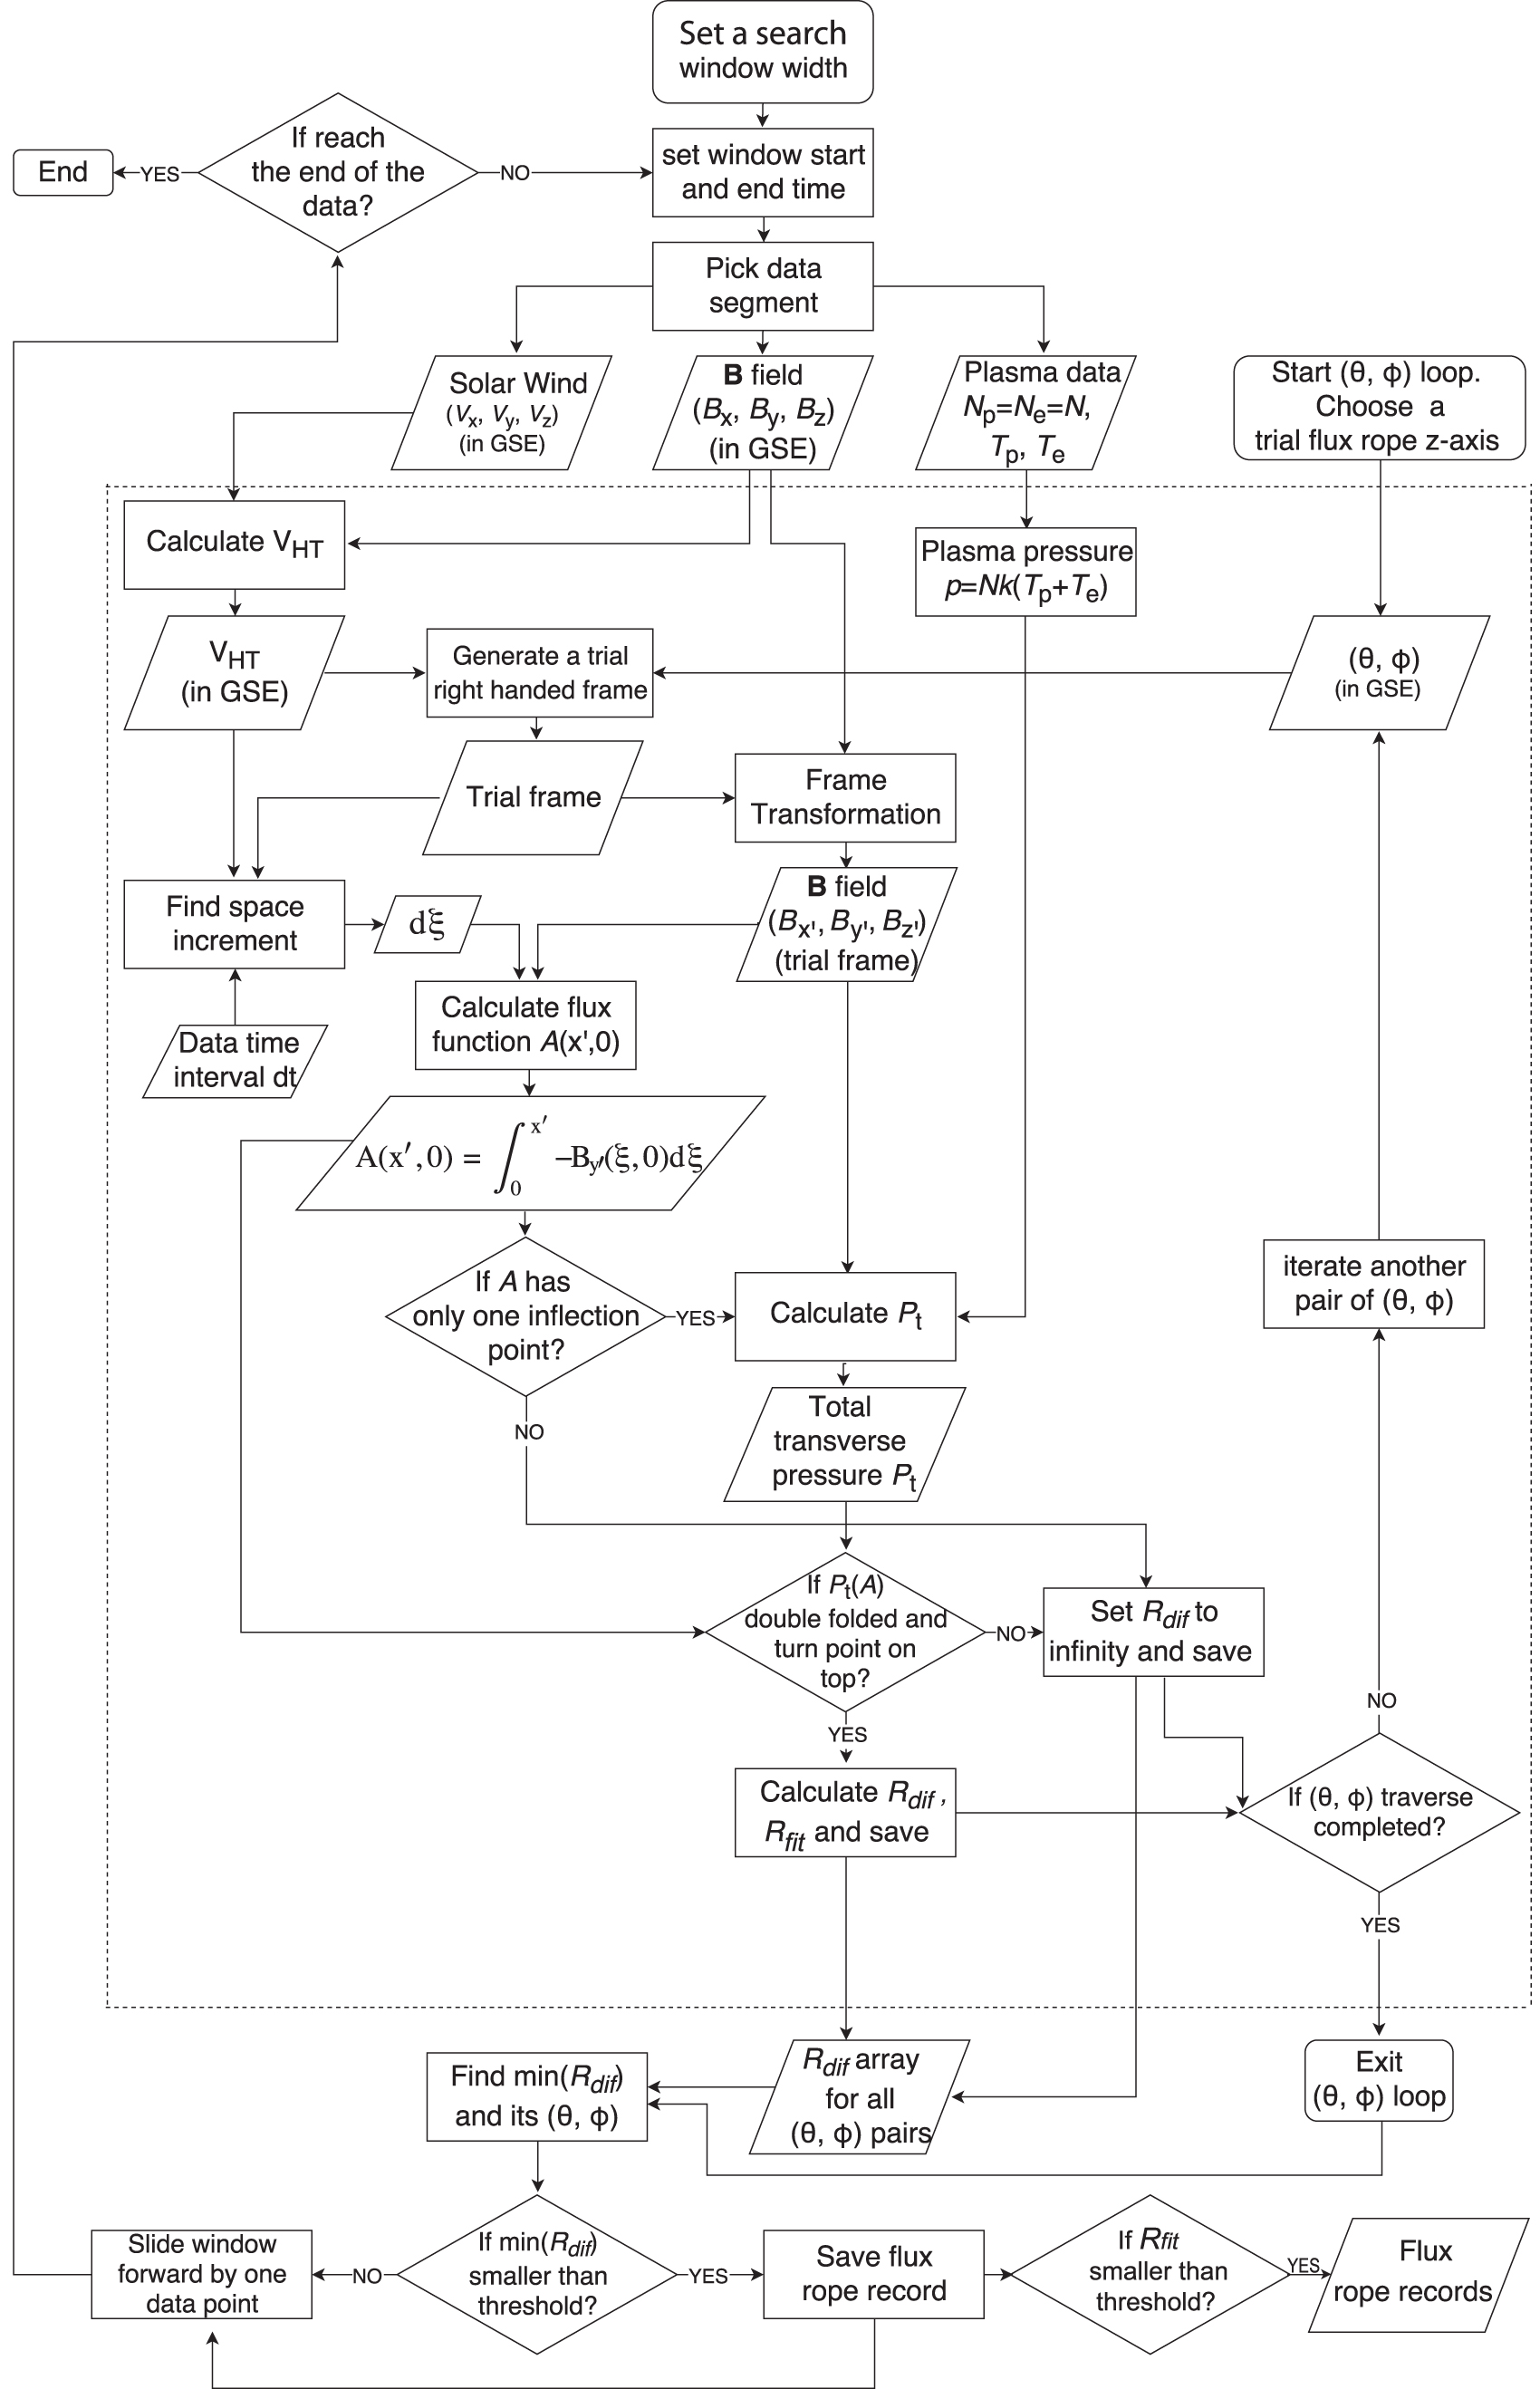
\includegraphics[width=0.8\textwidth]{Figures/fluxrope_algorithm.jpg}
    \caption[Flowchart of GS-reconstruction based automated detection algorithm]{Flowchart schematic of the automated detection algorithm of small-scale magnetic flux ropes, as implemented by \cite{Hu:2018} and \cite{Zheng:2018}.}
    \label{fig:flowchart}
\end{figure}


\end{document}
